\documentclass[a4paper,11pt,oneside]{book}
\usepackage{listings}
\usepackage[utf8]{inputenc}
\usepackage[spanish]{babel}
\usepackage{float}
\usepackage{enumitem}

\usepackage{changepage}

\usepackage{rotating}





\setcounter{secnumdepth}{3}


\decimalpoint
\usepackage{dcolumn}
\newcolumntype{.}{D{.}{\esperiod}{-1}}
\makeatletter
\addto\shorthandsspanish{\let\esperiod\es@period@code}
\makeatother

\RequirePackage{verbatim}
\usepackage{fancyhdr}
\usepackage{graphicx}
\usepackage{afterpage}

\usepackage{longtable}

\usepackage[pdfborder={0 0 0}]{hyperref} % referencia


% ********************************************************************
% Re-usable information
% ********************************************************************
\newcommand{\myTitle}{Aplicación para la gestión del hogar en piso de estudiantes \xspace}
\newcommand{\myDegree}{Grado en Ingeniería Informática\xspace}
\newcommand{\myName}{Sergio Muñoz Gómez \xspace}
\newcommand{\myProf}{María Luisa Rodríguez Almendros \xspace}
\newcommand{\myFaculty}{Escuela Técnica Superior de Ingenierías Informática y de Telecomunicación\xspace}
\newcommand{\myFacultyShort}{E.T.S. de Ingenierías Informática y de Telecomunicación\xspace}
\newcommand{\myDepartment}{Departamento de Lenguajes y Sistemas Informáticos\xspace}
\newcommand{\myUni}{\protect{Universidad de Granada}\xspace}
\newcommand{\myLocation}{Granada\xspace}
\newcommand{\myTime}{\today\xspace}
\newcommand{\myVersion}{Version 0.1\xspace}

\hypersetup{
	pdfauthor = {\myName (email (en) ugr (punto) es)},
	pdftitle = {\myTitle},
	pdfsubject = {},
	pdfkeywords = {palabra_clave1, palabra_clave2, palabra_clave3, ...},
	pdfcreator = {LaTeX con el paquete ....},
	pdfproducer = {pdflatex}
}

\usepackage{url}
\usepackage{colortbl,longtable}
\usepackage[stable]{footmisc}
\usepackage{index}
\usepackage{appendix}
\usepackage{hyperref}
\usepackage{titlesec}
\usepackage[utf8]{inputenc} % Para caracteres en español
\usepackage[spanish]{babel} % Para la correcta separación de sílabas y etiquetas en español
\usepackage{graphicx}
\usepackage{amssymb}
\usepackage{tabularx} 
\usepackage{pdflscape} 
\setlength{\parskip}{10pt}
\usepackage{rotating}
\usepackage{float}
\usepackage{xcolor}

% Configuración de enlaces
\hypersetup{
    colorlinks=true,
    linkcolor=black,
	urlcolor = black, 
    citecolor=black
}



\makeindex


\pagestyle{fancy}
\fancyhf{}
\fancyhead[LO]{\leftmark}
\fancyhead[RE]{\rightmark}
\fancyhead[RO,LE]{\textbf{\thepage}}
\renewcommand{\chaptermark}[1]{\markboth{\textbf{#1}}{}}
\renewcommand{\sectionmark}[1]{\markright{\textbf{\thesection. #1}}}


\usepackage{fancyhdr}
\pagestyle{fancy}
\fancyhf{} % Limpia el encabezado y pie de página de configuraciones previas
\fancyfoot[C]{\thepage} % Centra el número de página en el pie de página
\renewcommand{\headrulewidth}{0pt} % Elimina la línea del encabezado
\renewcommand{\footrulewidth}{0pt} % Elimina la línea del pie de página si existe

% Corrige cualquier espacio adicional alrededor del área del pie de página que podría desplazar el número de la página
\fancyfootoffset{0pt}


\usepackage{booktabs} % Para obtener líneas horizontales mejoradas
\usepackage[table]{xcolor}
\usepackage{eurosym}

\usepackage{apacite}
\bibliographystyle{apacite}


\setlength{\headheight}{1.5\headheight}
\begin{document}
\begin{titlepage}
 
 
\newlength{\centeroffset}
\setlength{\centeroffset}{-0.5\oddsidemargin}
\addtolength{\centeroffset}{0.5\evensidemargin}
\thispagestyle{empty}

\noindent\hspace*{\centeroffset}\begin{minipage}{\textwidth}

\centering

\includegraphics[width=0.9\textwidth]{imagenes/logo_ugr.jpg}\\[1.4cm]

\textsc{ \Large TRABAJO FIN DE GRADO\\[0.2cm]}
\textsc{ INGENIERÍA INFORMÁTICA}\\[1cm]
% Upper part of the page
% 
% Title
{\Huge\bfseries Aplicación para la gestión del hogar en piso de estudiantes \\
}
\noindent\rule[-1ex]{\textwidth}{3pt}\\[3.5ex]
\end{minipage}

\vspace{2.5cm}
\noindent\hspace*{\centeroffset}\begin{minipage}{\textwidth}
\centering

\textbf{Autor}\\ {Sergio Muñoz Gómez}\\[2.5ex]
\textbf{Directores}\\
{María Luisa Rodríguez Almendros}\\[2cm]

\includegraphics[width=0.3\textwidth]{imagenes/etsiit_logo.png}\\[0.1cm]
\textsc{Escuela Técnica Superior de Ingenierías Informática y de Telecomunicación}\\
\textsc{---}\\
Granada, Enero de 2025
\end{minipage}
%\addtolength{\textwidth}{\centeroffset}
%\vspace{\stretch{2}}
\end{titlepage}




\thispagestyle{empty}

\clearpage
\setcounter{page}{2}
\chapter*{}
%\thispagestyle{empty}
%\cleardoublepage

%\thispagestyle{empty}





\thispagestyle{empty}
\vspace{-5cm}

\begin{center}
{\large\bfseries Aplicación para la gestión del hogar en piso de estudiantes}\\
\end{center}
\begin{center}
Sergio Muñoz Gómez\\
\end{center}

%\vspace{0.7cm}
\noindent{\textbf{Palabras clave}: gestión, hogar, software, iteraciones}\\

\vspace{0.7cm}
\noindent{\textbf{Resumen}}\\

Poner aquí el resumen.
\cleardoublepage


\thispagestyle{empty}


\begin{center}
{\large\bfseries Project Title: Project Subtitle}\\
\end{center}
\begin{center}
Sergio Muñoz Gómez\\
\end{center}

%\vspace{0.7cm}
\noindent{\textbf{Keywords}: management, home, software, iterations}\\

\vspace{0.7cm}
\noindent{\textbf{Abstract}}\\

Write here the abstract in English.

\chapter*{}
\thispagestyle{empty}

\noindent\rule[-1ex]{\textwidth}{2pt}\\[4.5ex]

Yo, \textbf{Sergio Muñoz Gómez}, alumno de la titulación INGENIERÍA INFORMÁTICA de la \textbf{Escuela Técnica Superior
de Ingenierías Informática y de Telecomunicación de la Universidad de Granada}, con DNI 76062609E, autorizo la
ubicación de la siguiente copia de mi Trabajo Fin de Grado en la biblioteca del centro para que pueda ser
consultada por las personas que lo deseen.

\vspace{6cm}

\noindent Fdo: Sergio Muñoz Gómez

\vspace{2cm}

\begin{flushright}
Granada a 20 de Enero de 2025 .
\end{flushright}


\chapter*{}
\thispagestyle{empty}

\noindent\rule[-1ex]{\textwidth}{2pt}\\[4.5ex]

D. \textbf{María Luisa Rodríguez Almendros}, Profesora del Área de Ingeniería del Software del Departamento de Lenguajes y Sistemas Informáticos de la Universidad de Granada.

\vspace{0.5cm}

\textbf{Informan:}

\vspace{0.5cm}

Que el presente trabajo, titulado \textit{\textbf{Aplicación para la gestión del hogar en piso de estudiantes}},
ha sido realizado bajo su supervisión por \textbf{Sergio Muñoz Gómez}, y autorizamos la defensa de dicho trabajo ante el tribunal
que corresponda.

\vspace{0.5cm}

Y para que conste, expiden y firman el presente informe en Granada a 20 de Enero de 2025 .

\vspace{1cm}

\textbf{Los directores:}

\vspace{4cm}

\noindent \textbf{María Luisa Rodríguez Almendros}

\chapter*{Agradecimientos}
\thispagestyle{empty}

       \vspace{1cm}


En primer lugar quiero dar mis agradecimientos a mi familia, gracias por apoyarme siempre en todas las decisiones que he tomado
durante mi vida. Gracias por confiar en mí y por estar siempre a mi lado en los momentos más difíciles. Gracias por hacerme sentirme 
orgulloso de todos los logros que he conseguido y por darme ánimos en los momentos en los que las cosas no salían como esperaba.
Gracias por hacerme ver que todo es posible si se lucha por ello. Gracias por enorgullecerme de ser parte de esta familia.

En segundo lugar quiero agradecer a los amigos que me ha dado esta carrera, en concreto a Julia, Juan y Salma. Gracias por haberme enseñado 
lo que es la amistad incondiconal, gracias por todo el aprendizaje que me habeis dado y por haberme ayudado en los momentos en los que más lo he necesitado.
Gracias por haberme hecho reir y por haberme hecho ver que la vida es mucho más bonita si se comparte con amigos. Gracias por haberme hecho sentirme 
orgulloso de ser quien soy. Estoy muy orgullo de ser vuestro amigo.

No quiero olvidarme de mis compañeras de piso. Carla, Elena, Sandra, gracias por haberme hecho sentir como en casa desde el primer día.
Gracias por haberlo hecho todo tan fácil y por haberme ayudado en todo lo que he necesitado. Lo que empezó siendo una convivencia ha pasado a ser una familia. 

Por último quiero agradecer a mi tutora, María Luisa Rodríguez Almendros, por haberme guiado y ayudado en la realización de este trabajo. Este proyecto
no hubiera sido posible sin su ayuda y sin su apoyo.

Gracias a todos por haberme ayudado a llegar hasta aquí. Este trabajo es también vuestro.
\tableofcontents
\listoffigures
\listoftables

%\mainmatter
\setlength{\parskip}{5pt}

% Contenido Principal

\chapter{Introducción}
\label{cap:introduccion}




\section{Motivación}
\label{sec:motivacion}

La mayoría de estudiantes enfrentan dificultades para gestionar adecuadamente su hogar debido a la falta de tiempo, ya que gran parte de su jornada
está dedicada a sus estudios. Esta situación convierte la organización y la realización de tareas domésticas en un problema, pues estas actividades requieren 
una planificación cuidadosa y tiempo para llevarlas a cabo. Por otro lado, la gestión de los gastos compartidos puede resultar especialmente compleja en un entorno 
de estudiantes, ya que es común que cada miembro del hogar se encargue de diferentes pagos. Esto puede generar confusiones y equivocaciones, 
respectoa a quién ha pagado ciertos gastos y qué cantidades están pedientes, lo que agrava aún más la dificultad de una correcta
administación del hogar.

Después de 5 años viviendo de manera independiente, he experimentado de primera mano las dificultades de gestionar un hogar compartido con otros estudiantes o trabajadores. En numerosas ocasiones 
el tiempo libre del que disponíamos no se ha destinado a la organización del hogar. Aunque las tareas se asignaban semanalmente, no siempre se cumplían, ya sea
por falta de tiempo y o por descuidos. Además, la administación de los gastos ha sido, en muchas ocasiones, caótica, ya que no siempre se llevaba un control adecuado sobre quién ha pagado qué,
y algunas personas solían olvidar devolver el dinero a tiempo.  

En la actualidad, aproximadamente el \textbf{87\% de los jovenes emancipados en España viven comparten vivienda}, segun un estudio del portal HuffPost. \cite{huffpost2025}. Además, el 31\% de 
quienes alquilan una habitación en un piso compartido cohabitan con otras tres personas. \cite{ndp2024}. Por tanto, la necesidad de una aplicación que facilite la organización y gestión del hogar en pisos de estudiantes es evidente.

Actualmente no existe ninguna aplicación que ofrezca una solución integral tanto para la gestión de las tareas domesticas como para la gestión de los gastos. Las aplicaciones
disponibles abordan estos aspectos por separado. Además la mayoría de ellas están orientadas a hogares familiares donde la distribución de las tareas no se gestiona de la misma forma que 
en los pisos de estudiantes. Por eso es fundamental desarrollar una aplicación que integre todas estas funcionalidades, dirigida específicamente a estudiantes o trabajadores que compartan vivienda.

La aplicación que quiero desarrollar estará diseñada para ayudar a estudiantes y trabajadores que compartan vivienda,
proporcionando una solución integrada que facilite tanto la organización de las tareas domésticas como la administración de gastos compartidos.
En un entorno de convivencia, la asignación de tareas suele complicarse debido a los horarios irregulares y las diferentes cargas de estudio o trabajo de cada persona.
Esta aplicación permitirá a asignar tareas de manera equitativa y flexible, estableciendo recordatorios y notificando a cada miembro sobre las responsabilidades
asignadas para mejorar el cumplimiento y la colaboración en el hogar. 

Por otra parte, la aplicación incluirá un sistema de gestión de gastos compartidos, donde se registrarán todos los pagos realizados
y las cantidades que se deben por cada persona. Esto reducirá las confusiones y facilitará un control transparente y detallado de los 
gastos del hogar. En lugar de depender de otras aplicaciones o de anotaciones manuales, esta herramienta unificará ambos aspectos (tareas y gastos) 
en un solo lugar, simplificando la administración y ayudando a la organización en hogares compartidos. 

\section{Objetivos del proyecto}
\label{sec:objetivos}

El objetivo principal del proyecto es desarrollar una aplicación móvil para facilitar a los estudiantes la organización y gestión eficiente de su hogar, ofreciendo soluciones que aborden las dificultades 
que puedan surgir en la planificación y distribución de responsabilidades. Para poder alcanzar este objetivo, podemos diferenciar una serie de objetivos específicos:

\begin{itemize}
	\item\textbf{Objetivo 1: Análisis de la gestión de hogares compartidos y gestión de gastos.}
	\begin{itemize}
		\item \textbf{Descripción:} Búsqueda de información sobre los problemas más comunes que surgen en la gestión de hogares compartidos y en la gestión de gastos.
	\end{itemize} 

	\item \textbf{Objetivo 2: Estudio de aplicaciones similares}
	\begin{itemize}
		\item \textbf{Descripción:} Estudio del mercado actual de aplicaciones similares con el fin de identificar funcionalidades innovadoras que puedan ser incorporadas en nuestra aplicación.
	\end{itemize}

	\item \textbf{Objetivo 3: Análisis de las tecnologías a utilizar}
	\begin{itemize}
		\item \textbf{Descripción:} Investigar cuáles son las tecnologías más adecuadas para la implementación del proyecto.
	\end{itemize}
	
	\item \textbf{Objetivo 4: Desarrollo e implementación de la aplicación}
	\begin{itemize}
		\item \textbf{Descripción:} Analizar, desarrollar y realizar pruebas en la aplicación con el fin de obtener los mejores resultados.
	\end{itemize}
	\item \textbf{Objetivo 5: Análisis de usabilidad y accesibilidad}
    \begin{itemize}
        \item \textbf{Descripción:} Realizar un análisis de usabilidad y accesibilidad para identificar posibles mejoras en la interfaz de usuario.
    \end{itemize}
	\item \textbf{Objetivo 6: Validación de la aplicación por usuarios reales}
	\begin{itemize}
		\item \textbf{Descripción:} Evaluar la aplicación en un entorno real para verificar si satisface las expectativas del usuario.
	\end{itemize}
  
\end{itemize}

\section{Estructura de la memoria}
\label{sec:estructura}

A continuación, se ofrece una visión general de la estructura y organización de la memoria. El contenido se ha dividido en los siguientes apartados:

\begin{enumerate}
	\item \textbf{Introducción.} En este apartado se presenta la motivación del proyecto y los objetivos que se pretenden alcanzar.
	\item \textbf{Planificación y presupuesto.} Descripción de la planificación del proyecto, que incluye las diferentes fases que se han llevado a cabo durante su desarrollo, así como el presupuesto estimado. 
	\item \textbf{Estado del arte.} Estudio sobre los principales temas relacionados con este proyecto, cómo analisis de aplicaciones similares, temas legales de protección de datos, etc.
	\item \textbf{Análisis de tecnologías.} Análisis de las posibles tecnologías que se pueden usar en la actualidad y eleeciión de las más adecuadas para el desarrollo de la aplicación.
	\item \textbf{Análisis de metodologías de desarrollo} Análisis de las posibles metodologías que existen y elección de las más adecuadas para el desarrollo de la aplicación.
	\item \textbf{Propuesta.} Se presenta la aplicación propuesta, detallando su análisis y diseño. Se detallan los requisitos funcionales y no funcionales, asi como los diagramas de casos de uso y de clases. Se incluyen también los mockups de la aplicación.
	\item \textbf{Desarrollo e implementación de la aplicación.} Se detalla el proceso de desarrollo de la aplicación. Se realizará siguiendo una metodología iterativa y se detallarán sus iteraciones.
	\item \textbf{Validación de la aplicación por usuarios reales.} Evaluación de la aplicación en un entorno real para verificar si satisface las expectativas del usuario.
	\item \textbf{Conclusiones y trabajo futuro.} Se presentan las conclusiones obtenidas a lo largo del proyecto y se proponen posibles líneas de trabajo futuro.
	\item \textbf{Bibliografía.} Referencias bibliográficas utilizadas en la elaboración de la memoria.

\end{enumerate}


\newpage
%
\chapter{Planificación y presupuesto}
\label{cap:planificacion}

\section{Fases}
\label{sec:fases}
La planificación del proyecto se estructurará en fases con el objetivo de garantizar un desarrollo organizado y eficiente, asegurando que cada etapa esté enfocada en el cumplimiento de objetivos específicos.

\subsection{Fase Inicial}
En esta fase se recopilará y definirá toda la información relacionada con el Capitulo 1, incluyendo la motivación para la realización del proyecto y la determinación de los objetivos que se pretenden alcanzar a lo largo del mismo. 

\subsection{Fase de Investigación}
Esta fase estará dedicada a la recopilación de información relevante para el desarrollo del proyecto. Se analizarán aplicaciones similares para demostrar la necesidad de una aplicación integral que cubra todas las funciones propuestas. 
Además se investigará aspectos como la gestión del tiempo en hogares compartidos y la administración de gastos entre personas que comparten un mismo domicilio.

Para garantizar que la aplicación cumpla con los requisitos legales, también se revisará la normativa vigente de protección de datos. Asímismo, se realizará un estudio 
de usabilidad y accesibilidad para asegurar que el diseño sea inclusivo y fácil de usar para todos los usuarios.

\subsection{Fase de Analisis}
En esta fase se llevará a cabo un análisis de las diferentes tecnologías que se pueden utilizar para el desarrollo de la aplicación, tanto para el frontend como para el 
backend, con el objetivo de selecionar las más adecuadas para el proyecto. Además, se definirán los requisitos que debe cumplir la aplicación para satisfacer las necesidades del usuario objetivo. Como
parte de esta fase, se elaborarán los casos de uso y los diagramas de secuencia del sistema.

\subsection{Fase de Diseño}
Esta fase estará enfocada en la creación de los prototipos de la aplicación. Se desarrollará un diagrama de arquitectura del sistema y bocetos para la interfaz gráfica. Además, se definirán 
los colores y las tipografías que se emplearán en la aplicación, garantizando un diseño responsive que permita su visualización en cualquier dispositivo.

\subsection{Fase de Desarrollo}
En esta fase se procederá a la implementación de la aplicación, siguiendo las tecnologías, metodologías y diseños definidos en las fases previas de análisis y diseño. Esta fase se dividirá en cuatro iteraciones,
ya que se empleará una metodología ágil para el desarrollo del proyecto. En cada iteración se determinarán las funcionalidades que se implementarán y se realizarán pruebas para garantizar 
que la aplicación cumple con los requisitos definidos en la fase de análisis.

Las pruebas serán realizadas por usuarios reales, concretamente jóvenes que comparten piso, para verificar que la aplicación satisface sus necesidades y resulta fácil de utilizar.

\subsection{Documentación}
Aunque no se considera una fase independiente, la documentación será un proceso continuo a lo largo de todo el proyecto. Se registrarán de manera detallada todas las actividades y resultados obtenidos en cada fase. 

\subsection{Diagrama de Gantt}
En esta tabla se específica la duración en horas de cada una de las tareas representadas en el diagrama de Gantt. Este diagrama representa 
la planificación temporal de las actividades del proyecto, donde cada celda corresponde a una semana del mes. La tabla presenta la cantidad de horas
dedicadas a cada tarea, mientras que el diagrama de Gantt muestra el periodo en el que se llevaron a cabo. 

\begin{table}[ht]
    \centering
    \resizebox{\textwidth}{!}{%
    \begin{tabular}{|l|c|}
        \hline
        \rowcolor[HTML]{C0C0C0} 
        \textbf{Tarea} & \textbf{Horas} \\ \hline
        Motivación & 1 \\ \hline
        Objetivos del proyecto & 2\\ \hline
        Estructura de la memoria  & 2 \\ \hline
        Planificación & 3 \\ \hline
        Presupuesto & 4\\ \hline
        Estudios sobre la gestión del hogar y las finanzas en viviendas compartidas & 20 \\ \hline
        Aplicaciones similares y comparativas  & 25 \\ \hline
        Legislación actual de protección de datos & 7 \\ \hline
        Estudio de usabilidad y accesibilidad & 12 \\ \hline
        Análisis de las tecnologías Frontend & 20 \\ \hline
        Analisis de las tecnologías Backend & 15 \\ \hline
        Análisis de las metodologías de desarrollo & 12 \\ \hline
        Explicación de la propuesta & 2 \\ \hline
        Análisis de la aplicación & 40 \\ \hline
        Diseño de la aplicación & 40 \\ \hline
        Elección de tecnologias & 2 \\ \hline
        Iteración 1 & 30 \\ \hline
        Iteración 2 & 45 \\ \hline
        Iteración 3 & 45 \\ \hline
    \end{tabular} %
    }
    \caption{Tabla de tareas y horas}

\end{table}

\newpage

\section{Presupuesto}
\label{sec:presupuesto}
En este apartado se detallarán los costes asociados al desarrollo del proyecto. Se incluirán los costes de hardware, software, licencias, servicios en la nube y otros gastos necesarios para la realización del proyecto.
Realizar un presupuesto en este proyecto es clave para planificar y gestionar los recursos de forma eficiente. Permite asegurarse de que las fases de desarrollo se puedan llevar a cabo con los medios disponibles. 
Además, ayuda a justificar las decisiones tomadas y evitar problemas por faltas de recursos asegurando que el proyecto sea viable y esté bien estructurado. 

\subsection{Recursos Hardware}
Los componentes hardware necesarios para el desarrollo del proyecto son un ordenador portátil y un teléfono móvil para realizar pruebas con la aplicación. 

\begin{itemize}
    \item \textbf{Ordenador:} TUF Gaming FX505DT\_FX505DT 
    \item \textbf{Teléfono Móvil:} Samsung Galaxy A51
\end{itemize}

\subsection{Recursos Software}
Las herramientas software que se utilizarán en el proyecto son las siguientes:
\begin{itemize}
    \item \textbf{Sistema Operativo:} Windows 11
    \item \textbf{IDE:} Visual Studio Code
    \item \textbf{Control de Versiones:} Git
    \item \textbf{Lenguajes de Programación:} Flutter, Dart
    \item \textbf{Diseño de diagramas UML:} Visual Paradigm
    \item \textbf{Diseño de Interfaces:} Figma
    \item \textbf{Sistema de Gestión de Base de Datos:} Firebase
    \item \textbf{Sistema de composición de texto:} LaTeX
\end{itemize}

\subsubsection{Recursos Humanos}
En este apartado se detallarán los gastos por la contratación de personal. 
Este proyecto será desarrollado por una única persona, un programador junior, que según \cite{Talent2025} tiene un coste de 21.000\euro al año, como la duración de este proyecto es de 6 meses, el coste total será de 10.500\euro.


\subsection{Licencias}
En este apartado se detallan las licencias software necesarias para llevar a cabo el desarrollo del proyecto. Aunque en este caso no supone ningún coste, 
ya que se utilizarán versiones gratuitas o herramientas sin coste, en un proyecto real sería imprescindible considerar el pago de las licencias. Esto garantizaría 
el acceso completo a todas las funcionalidades de las herramientas, además de cumplir con las normativas legales y éticas relaciondas con el uso del sotware. Las licencias de software que deberían considerarse en un proyecto real 
son las siguientes: 
\begin{itemize}
    \item \textbf{Windows 11:} Windows 11 Home License
    \item \textbf{Visual Paradigm:} Visual Paradigm Standard Edition
    \item \textbf{Figma:} Figma Professional
\end{itemize}

El resto de licencias necesarias para el desarrollo del proyecto son gratuitas, por lo que no se incluirán en el presupuesto.


\subsection{Costes indirectos}
En este apartado se engloba todos los gastos indirectos que incluyen los costes de electricidad, internet, espacio de trabajo, etc. 
Estos gastos indirectos suelen estimarse como un porcentaje adicional del coste directo total \textit{(entre 10\% y 20\%)}.
En este caso será un 15\% de los recursos humanos.

\subsection{Presupuesto Total}
El coste total del proyecto se obtiene sumando los costes de los recursos hardware, software, humanos, licencias y costes indirectos.

\begin{table}[H]
    \centering
    \begin{tabular}{|l|c|c|}
        \hline
        \rowcolor[HTML]{C0C0C0} 
        \textbf{Concepto} & \textbf{Coste Mensual} & \textbf{Coste Total} \\ \hline
        \textbf{Recursos Hardware} & - & 1.000 \euro \\ \hline
        Ordenador portátil & - & 800 \euro \\ \hline
        Teléfono móvil para pruebas & - & 200 \euro \\ \hline
        \textbf{Recursos Humanos} & 1.750\euro & 10.500 \euro \\ \hline
        Programador Junior (6 meses) & 1.750\euro & 10.500 \euro \\ \hline
        \textbf{Licencias} & 52,68\euro & 316,12\euro \\ \hline
        Windows 11 Home License & - & 145 \euro \\ \hline
        Visual Paradigm Standard Edition & 12,23\euro & 73,38\euro \\ \hline
        Figma Professional & 20,45\euro & 122,7\euro \\ \hline
        \textbf{Costes Indirectos} & 262,5\euro & 1.575\euro \\ \hline
        Electricidad & 50\euro & 300\euro \\ \hline
        Internet & 30\euro & 180\euro \\ \hline
        Espacio de trabajo (estimado) & 182,5\euro & 1.095\euro \\ \hline
        \textbf{Coste Total} & 2.065,18\euro & \textbf{13.391,12\euro} \\ \hline
    \end{tabular}
    \caption{Presupuesto detallado del proyecto}
    \label{tab:presupuesto_detallado}
\end{table}




\newpage
%
\chapter{Estado del arte}
\label{cap:arte}

\section{Aplicaciones similares y comparativas}
\label{sec:aplicaciones}

\subsection{Tricount}
\label{subsec:tricount}

Tricount es una aplicación diseñada para facilitar la gestión y el reparto de gastos entre varias personas. Es útil en sistuaciones,
donde un grupo de personas realiza gastos comunes, como en viajes o cenas. Es una aplicación bastante sencilla de usar, lo que la 
hace aún más popular entre los grupos de personas. Está disponible para Android e iOS y tiene también soporte web. 

\subsubsection{Funciones Principales}
\label{subsubsec:funciones}
\begin{enumerate}
    \item \textbf{Creación de un Tricount}
    \begin{enumerate}
        \item Configuración Inicial. Al iniciar un nuevo "Tricount" (grupo) se le da un nombre, se elige un tipo de divisa y se añade a los participantes.
        \item Acceso Compartido. Puede ser compartido entre todos los participantes a través de un enlace, lo que permite que cada uno pueda añadir sus gastos.
    \end{enumerate}
    \item \textbf{Añadir Gastos}
    \begin{enumerate}
        \item Registro de Gastos. Cualquier participante puede añadir un gasto en el tricount, especificando la cantidad, la categoría,
        quien pagó y para quien es ese gasto.
        \item División Personalizada. Tricount permite dividir los gastos de forma equitatica o personalizada, es decir, si el gasto es para todos o solo para algunos. 
        \item Comentarios. Se pueden añadir comentarios a cada pago.
    \end{enumerate}
    \item \textbf{Cálculo Automático}
    \begin{enumerate}
        \item Resumen de Balances. Se calcula automáticamente cúanto debe cada persona y a quien. 
        \item Balances Individuales. Cada participante puede ver su valance individual y cuánto ha gastado, cuánto le deben y cuánto le debe a otros.
    \end{enumerate}
    \item \textbf{Saldar Deudas}
    \begin{enumerate}
        \item Recomendaciones de Pagos. Tricount recomienda la mejor manera de saldar las deudas dentro del grupo, optimizando el número de 
        transsaciones necesarias.
        \item Pagos Parciales o Totales. Los participantes puedden registrar pagos parciales o totales dentro de la aplicación para mantener un
        seguimiento claro de lo que ha sido pagado y lo que queda pendiente.
    \end{enumerate}
\end{enumerate}

\subsubsection{Modo de Uso}
Una vez nos hayamos descargado la aplicación ya sea desde Google Play o App Store, lo primero 
que nos muestra es una pantalla de inicio como nos muestra la \textit{Figura \ref{principal}}.

\begin{figure}[ht]
    \centering
    \begin{minipage}{0.45\textwidth}
        \centering
        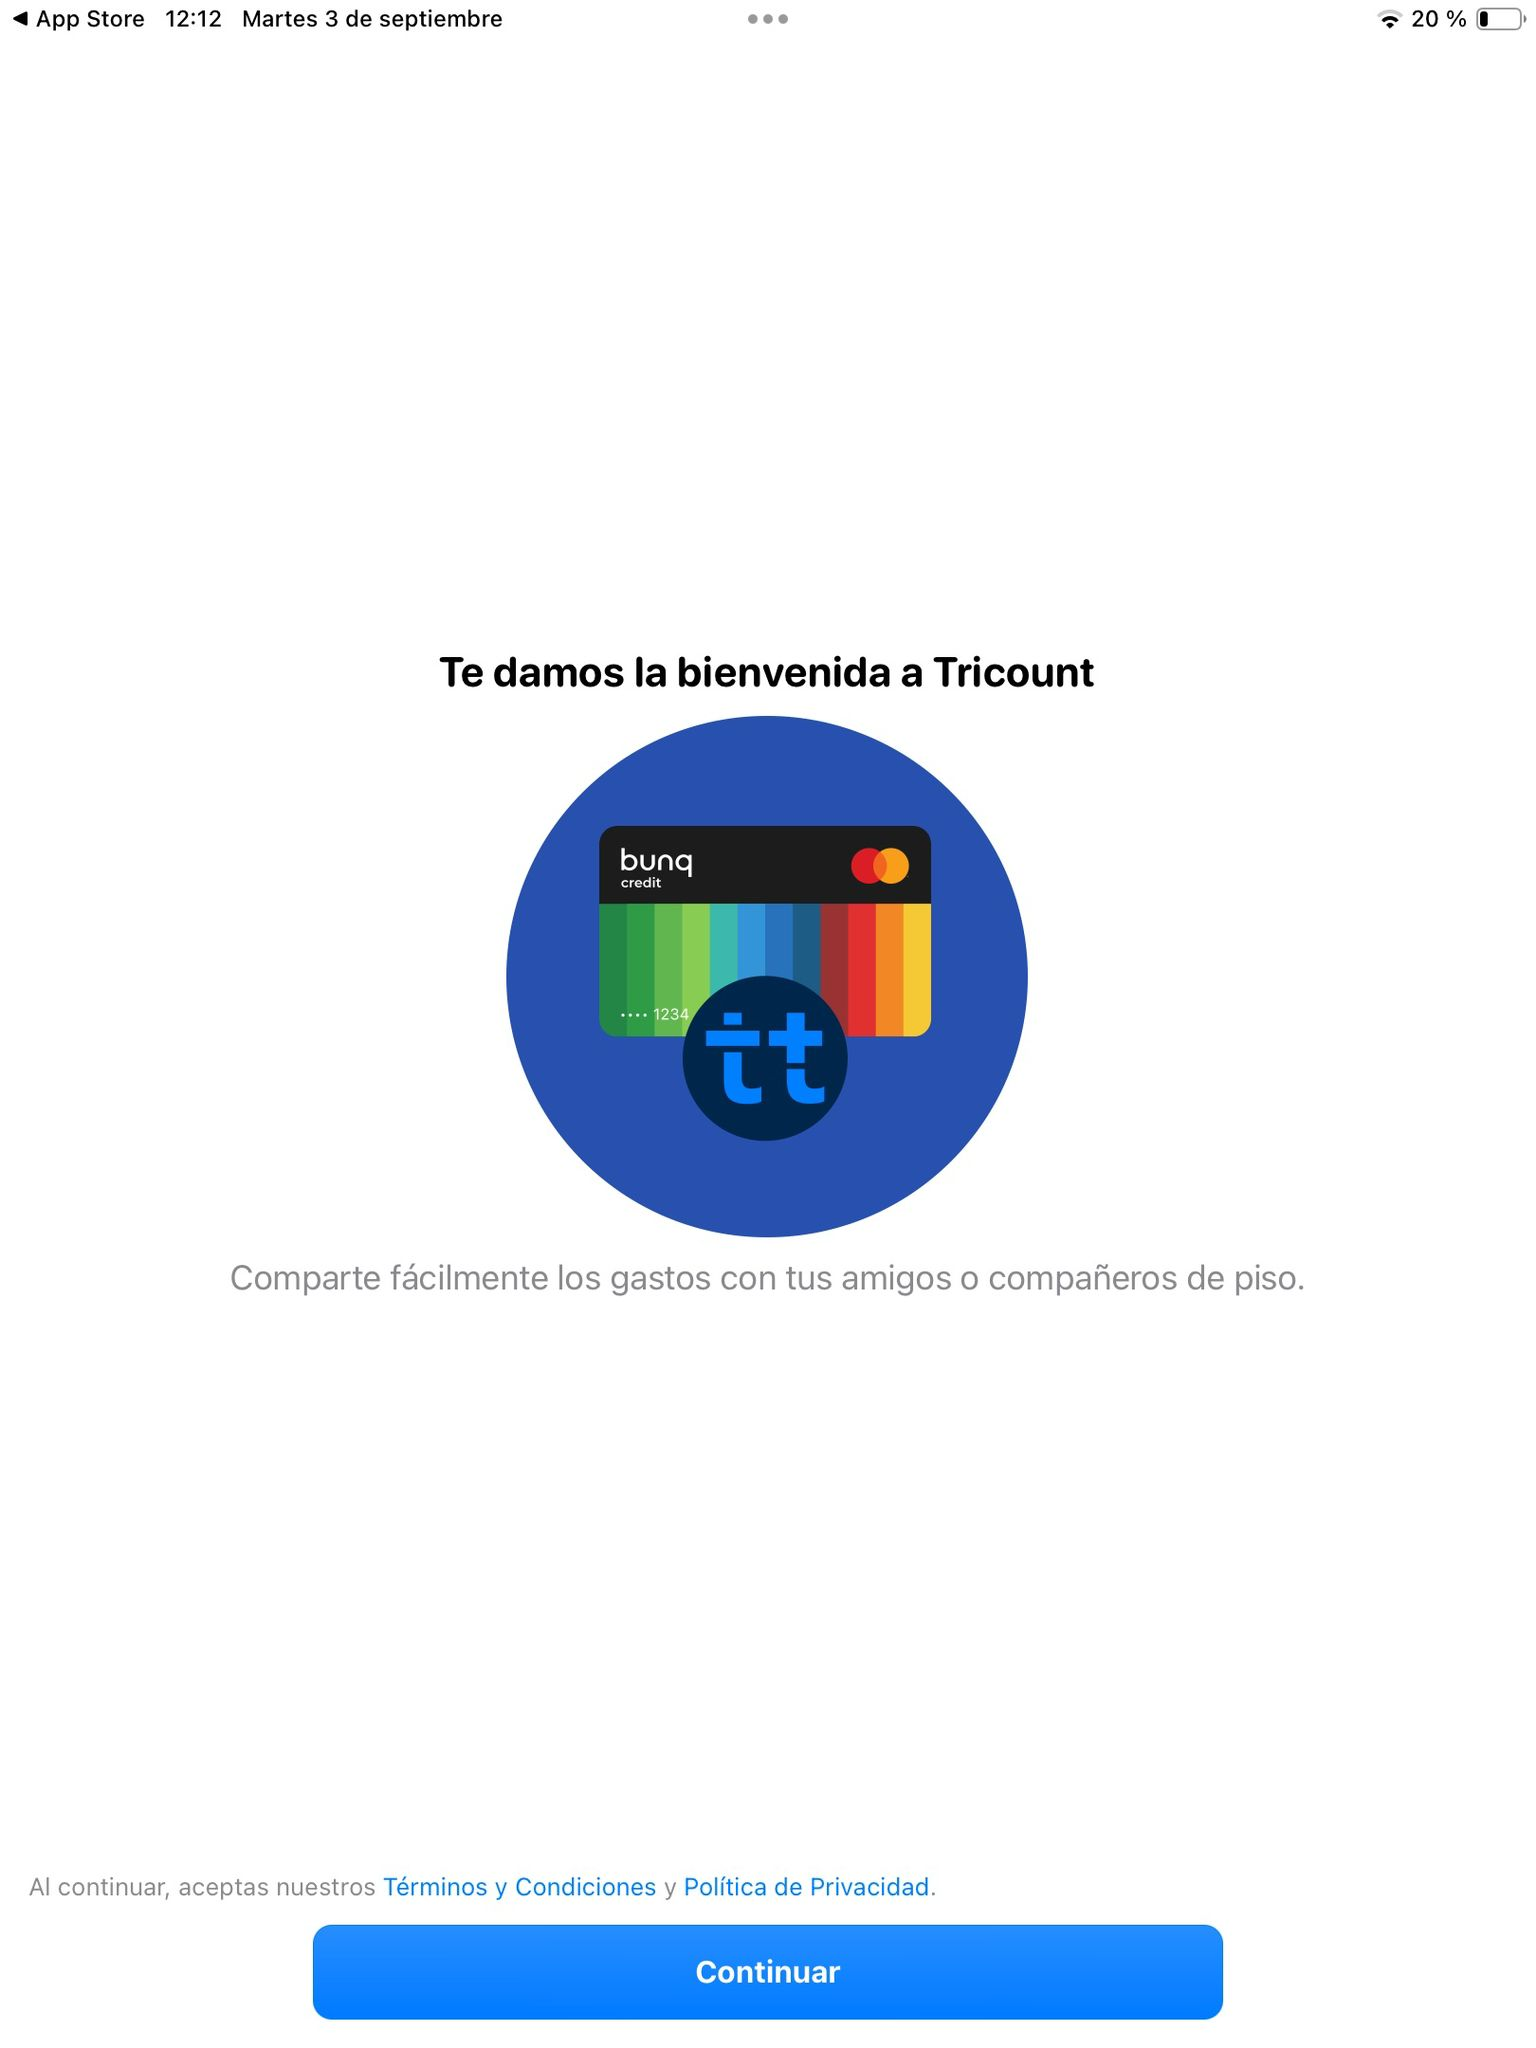
\includegraphics[width=\textwidth]{../capitulos/img/principal.jpg}
        \caption{Pantalla Inicio.}
        \label{principal}
    \end{minipage}
    \hfill
    \begin{minipage}{0.45\textwidth}
        \centering
        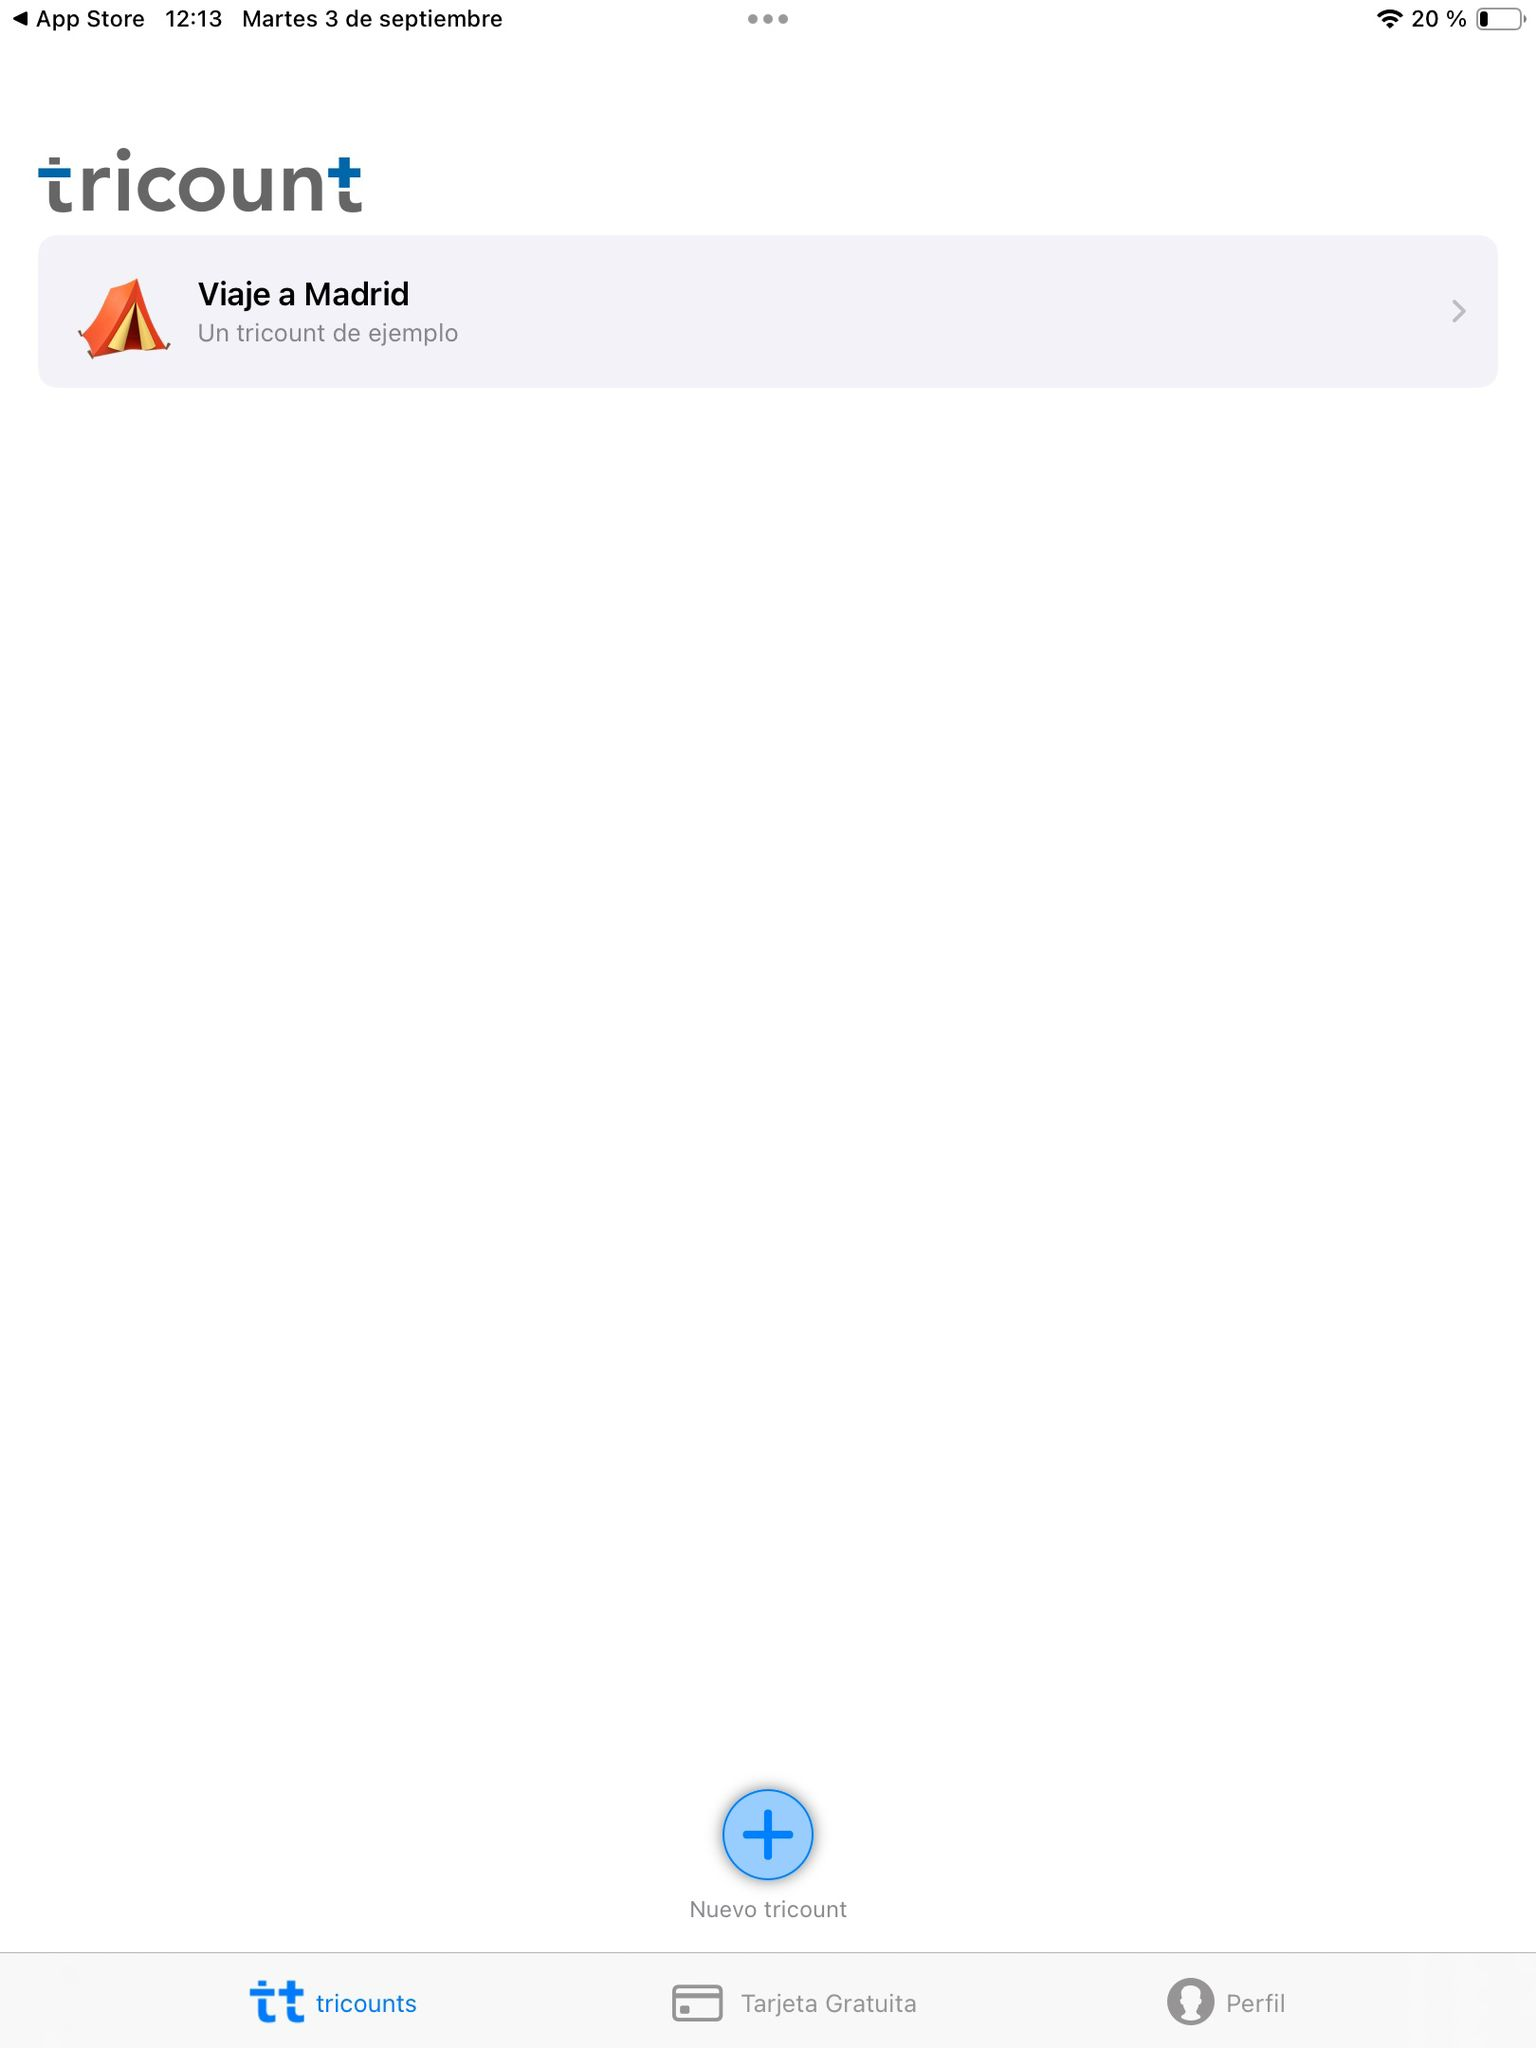
\includegraphics[width=\textwidth]{../capitulos/img/inicio.jpg}
        \caption{Lista de grupos.}
        \label{grupos}
    \end{minipage}
\end{figure}



Pulsado el botón de \textit{Continuar} nos muestra una pantalla donde 
nos sale una lista de los grupos que hemos creado o en los que estamos participando.
En este caso como es la primera vez que entramos solo nos muestra un grupo de ejemplo
(\textit{Figura \ref{grupos}}).


Para añadir un nuevo grupo, pulsamos el botón de \textit{Nuevo Tricount} 
y nos muestra una pantalla emergente donde nos da dos opciones, la primera 
es iniciar un Tricount (grupo) desde 0 y la otra es unirnos a un grupo ya existente (\textit{Figura \ref{nuevo}}).

\begin{figure}[ht]
    \centering
    \begin{minipage}{0.45\textwidth}
        \centering
        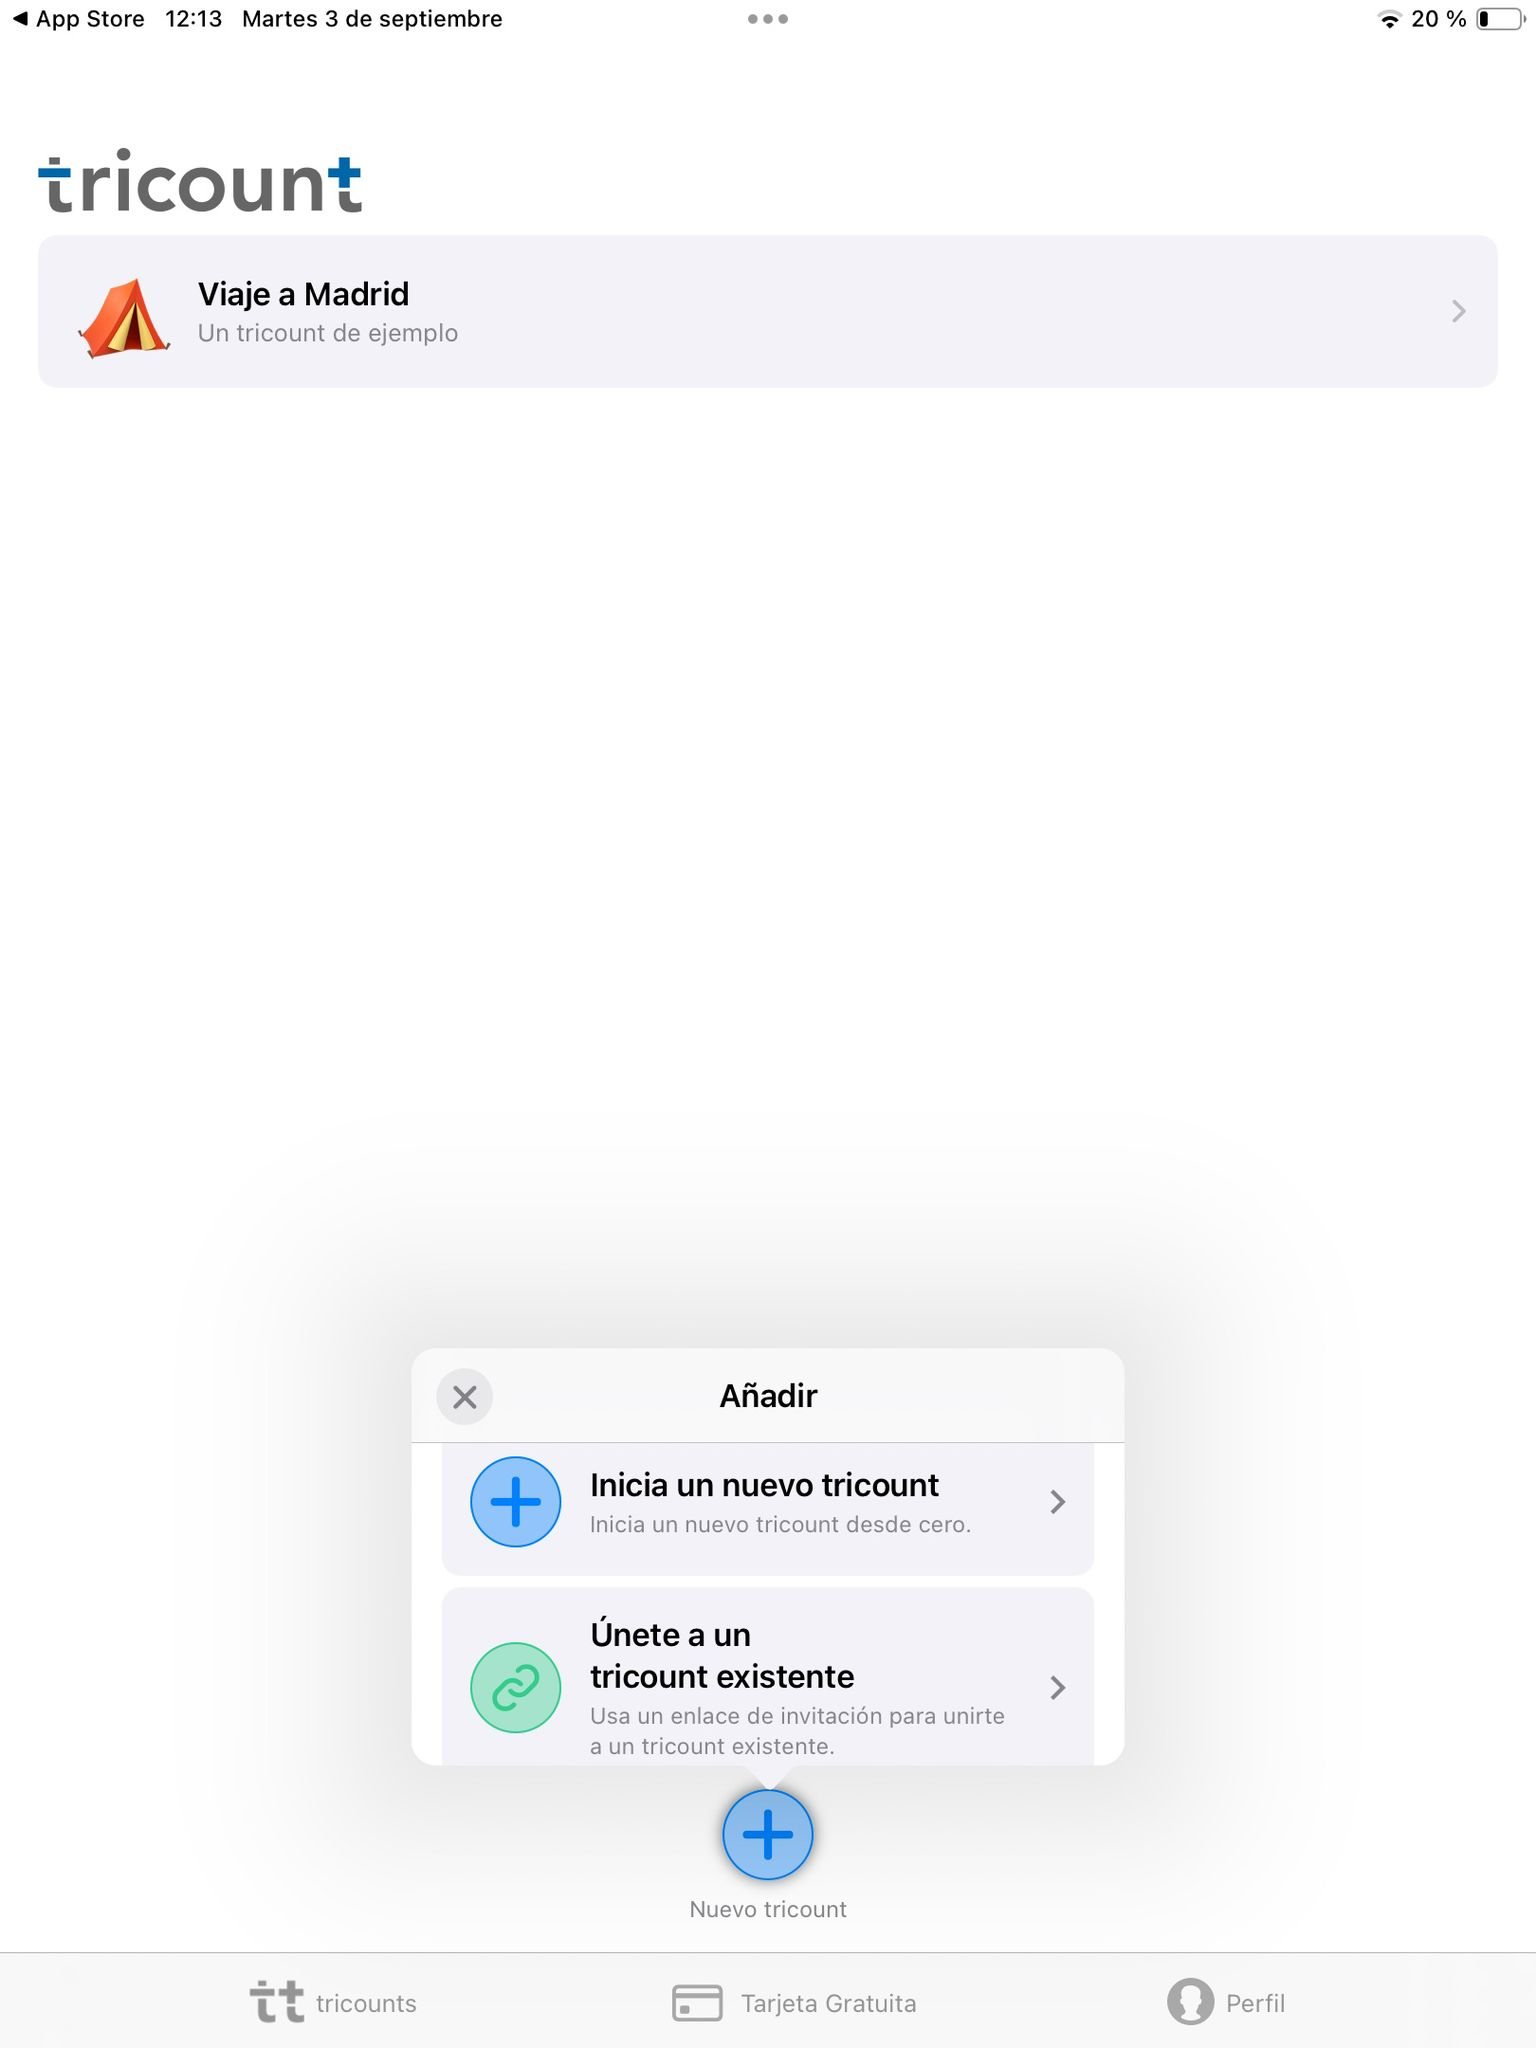
\includegraphics[width=\textwidth]{../capitulos/img/añadir.jpg}
        \caption{Añadir un nuevo grupo.}
        \label{nuevo}
    \end{minipage}
    \hfill
    \begin{minipage}{0.45\textwidth}
        \centering
        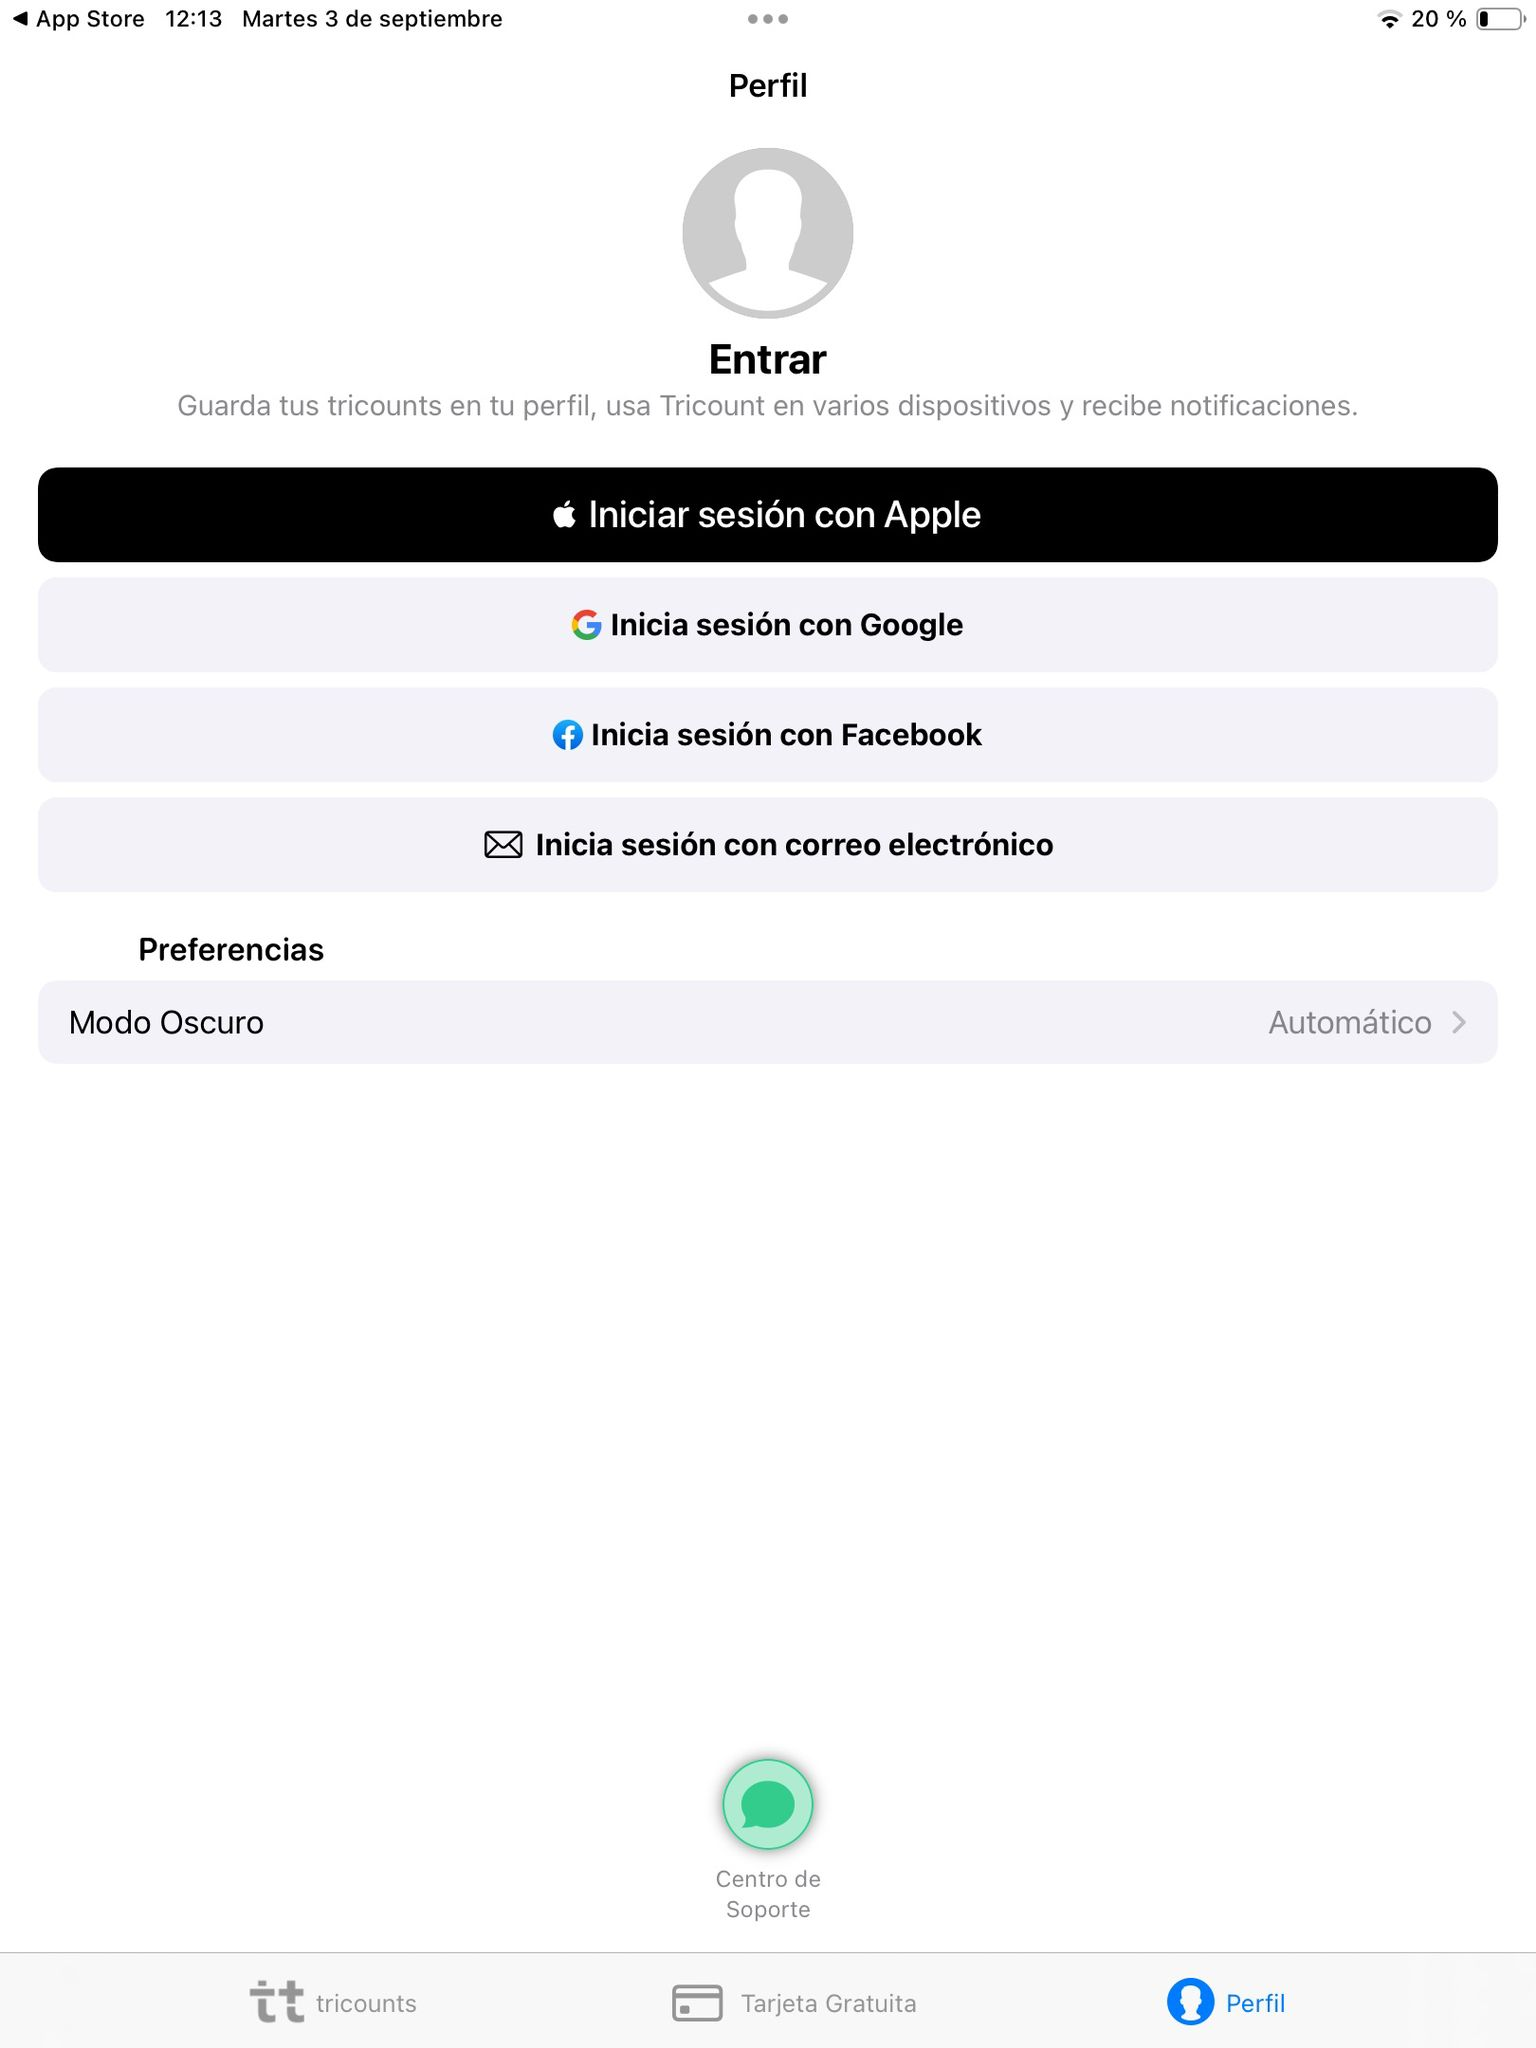
\includegraphics[width=\textwidth]{../capitulos/img/incio_sesion.jpg}
        \caption{Pantalla del perfil.}
        \label{perfil}
    \end{minipage}
\end{figure}


Otra de las pestañas que nos muestra es la del perfil, donde nos permite iniciar sesión y en caso de que ya estuvisemos registrado, 
se nos importan todos los grupos que estuvieran asociados a nuestra cuenta (\textit{Figura \ref{perfil}}). 
Ahora vamos a hablar de lo realmente importante de la aplicación y es de cómo crear un grupo y añadir gastos. Para ello después de 
pulsar el botón de \textit{Nuevo Tricount} nos da la opción de crear  un grupo desde 0, le damos un nombre, añadimos los miembros que van a
participar en el grupo y elegimos la divisa.(\textit{Figura \ref{crear_grupo}}). Una vez creado nos permite enviar un enlace a la gente que va a participar en el grupo
(\textit{Figura \ref{enlace}}).

\begin{figure}[ht]
    \centering
    \begin{minipage}{0.45\textwidth}
        \centering
        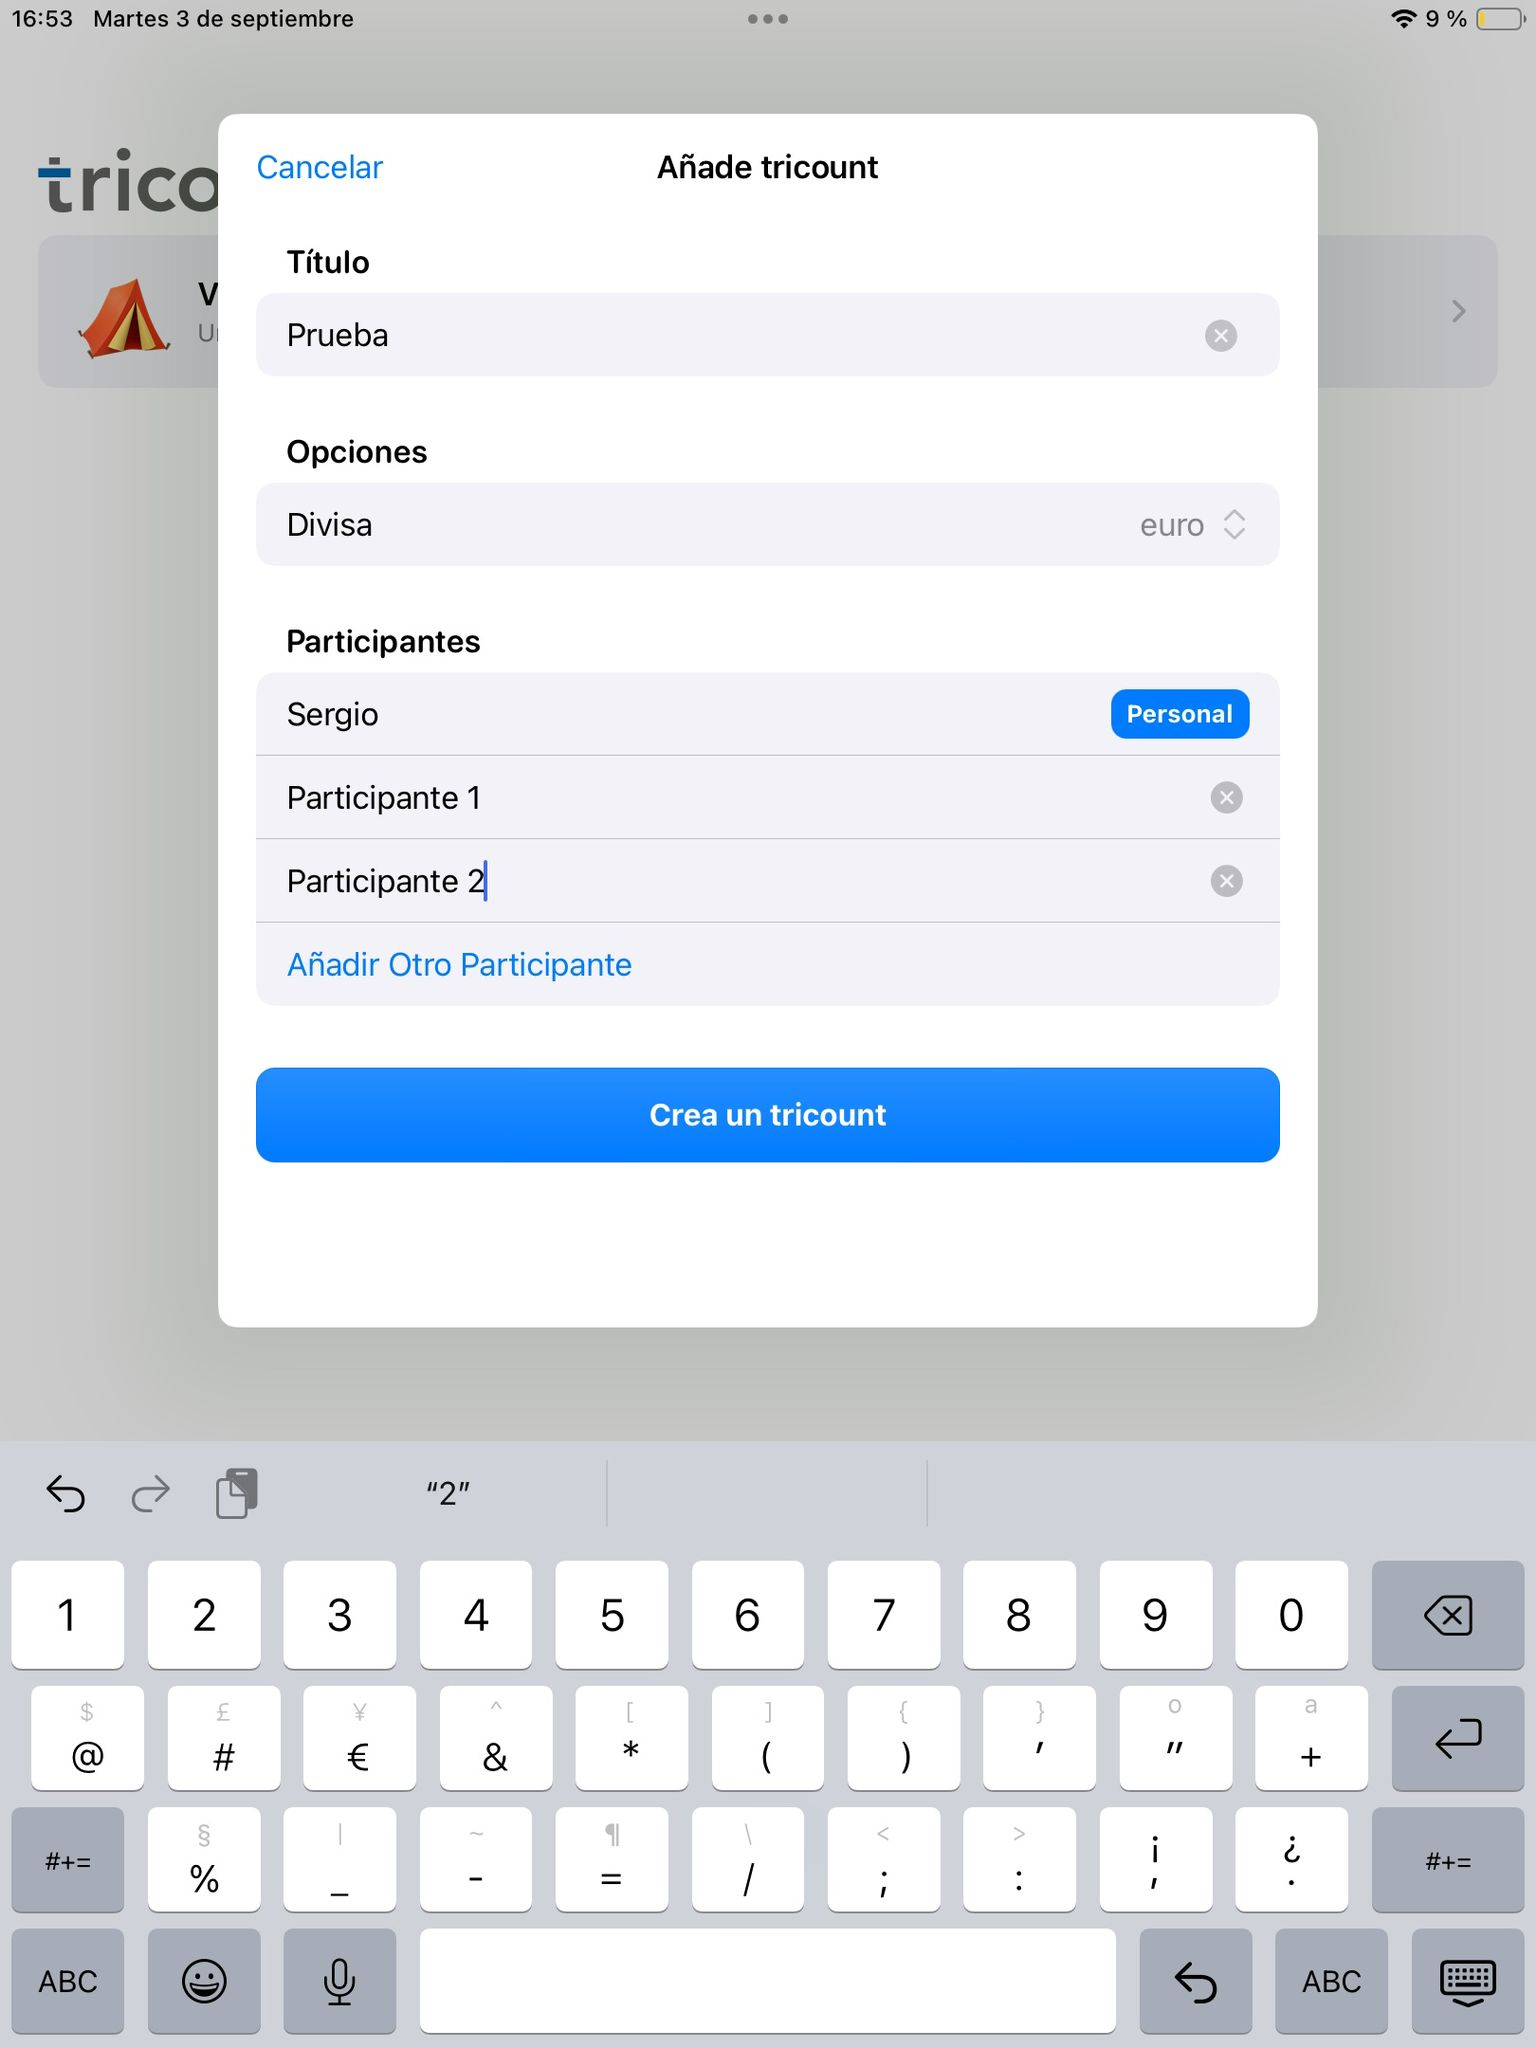
\includegraphics[width=\textwidth]{../capitulos/img/crear.jpg}
        \caption{Detalles de un nuevo grupo.}
        \label{crear_grupo}
    \end{minipage}
    \hfill
    \begin{minipage}{0.45\textwidth}
        \centering
        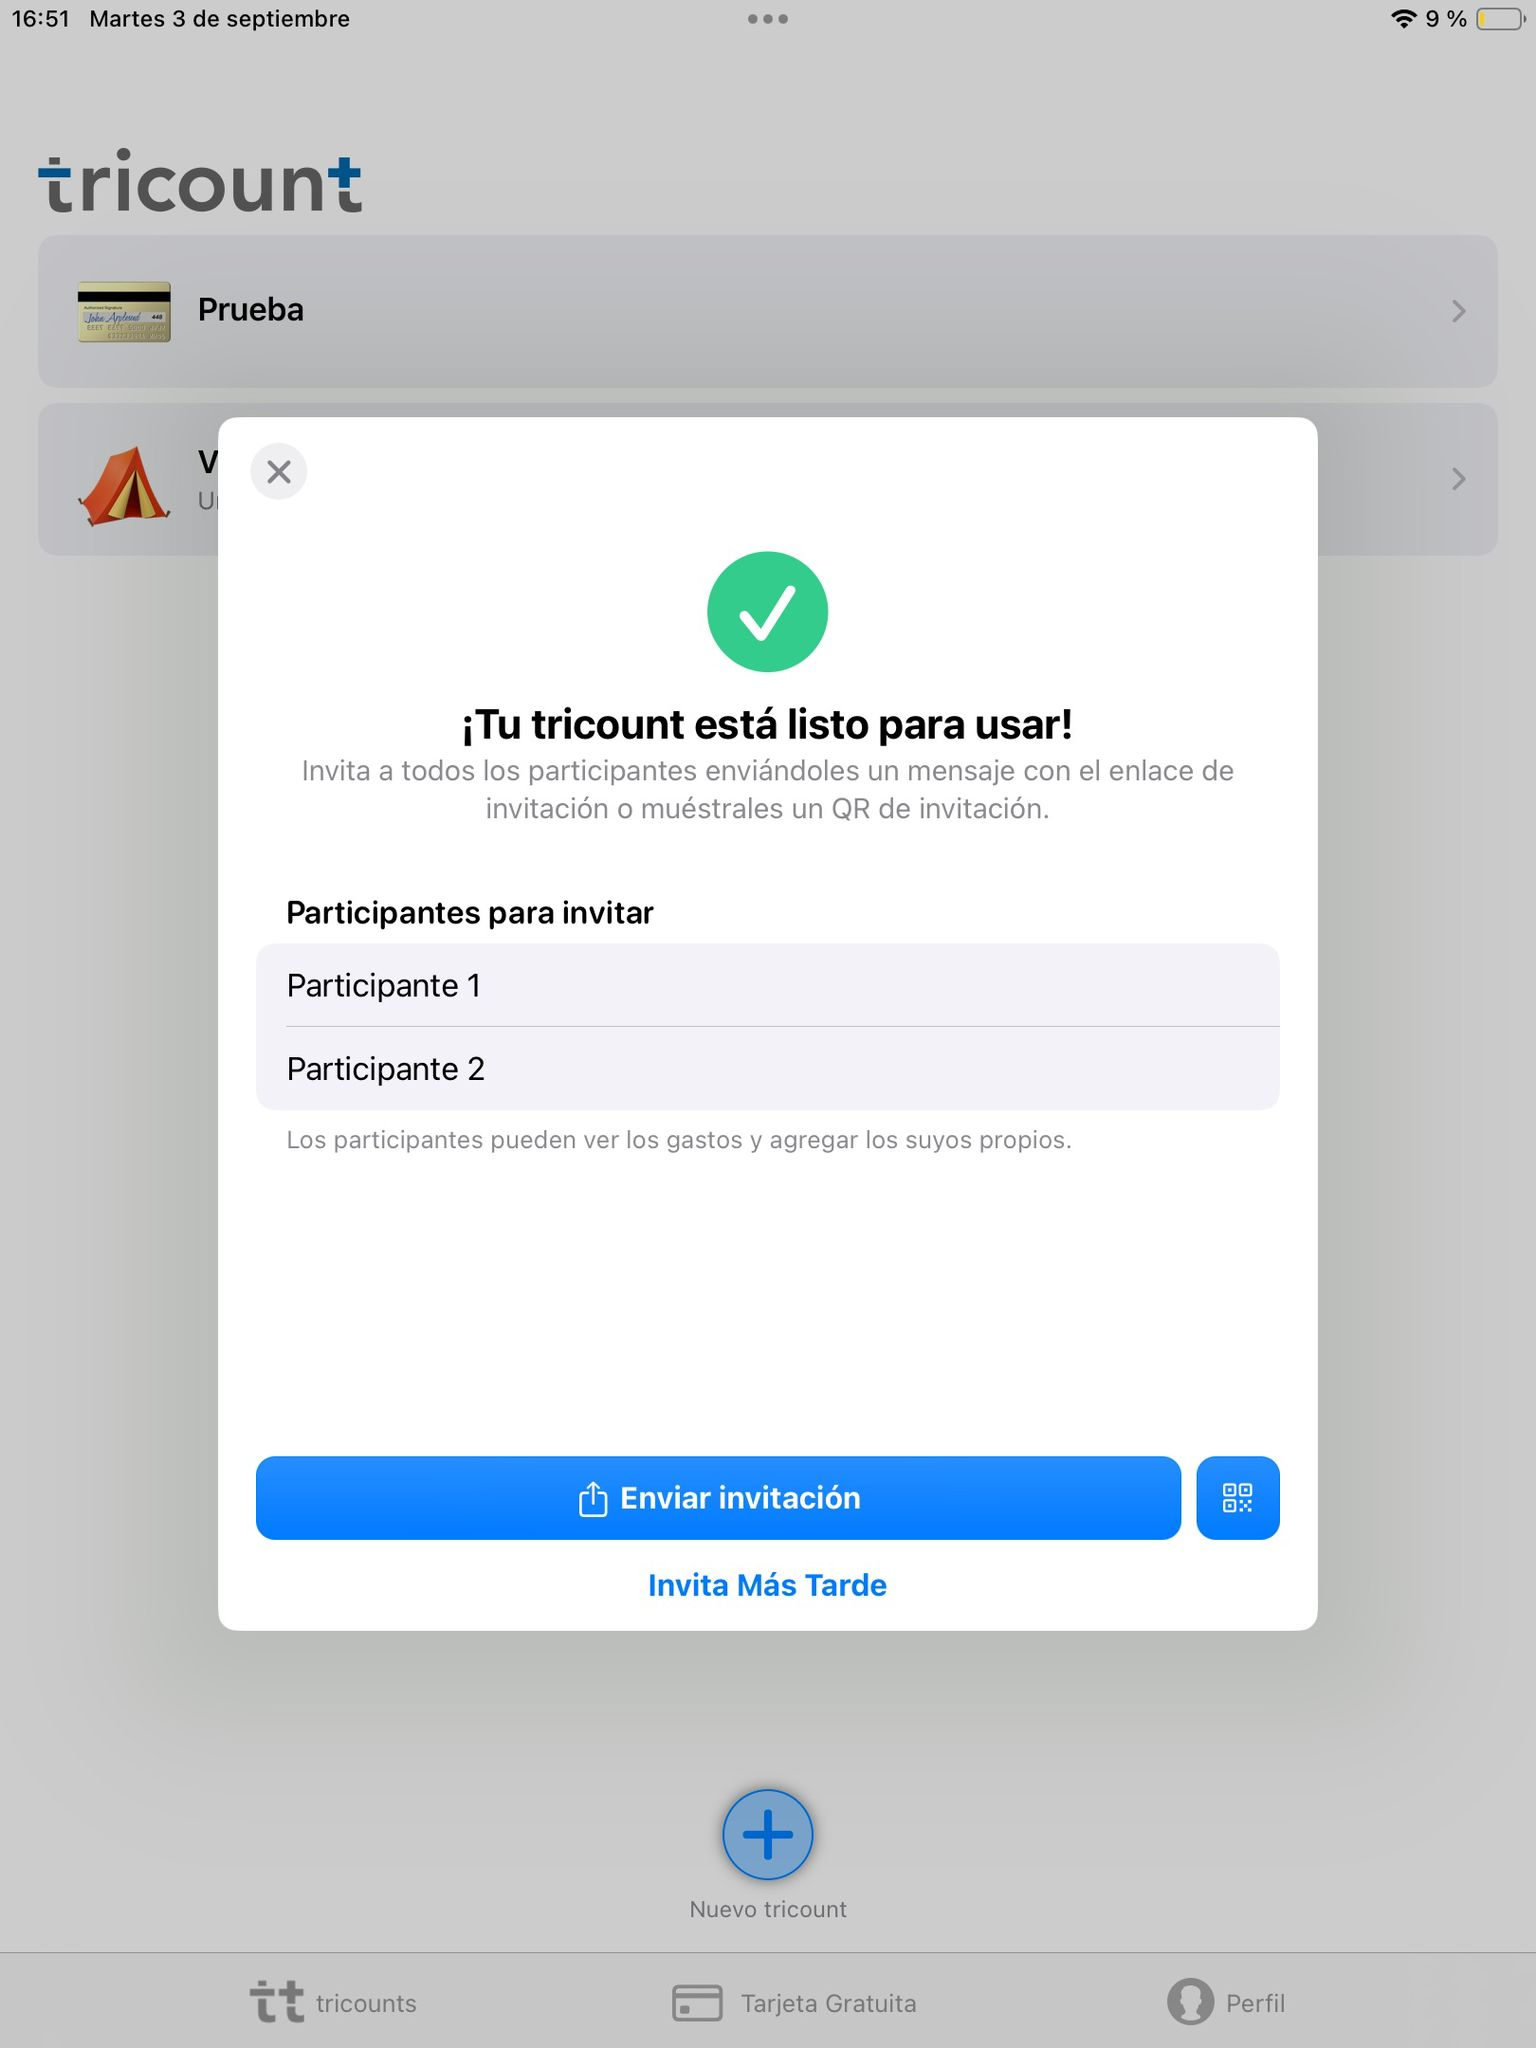
\includegraphics[width=\textwidth]{../capitulos/img/creado.jpg}
        \caption{Enviar invitación a los miembros del grupo.}
        \label{enlace}
    \end{minipage}
\end{figure}


Lo siguiente que vamos a hacer es añadir un gasto, para ello pulsamos el botón de \textit{Añadir un gasto}
y nos muestra una pantalla donde podemos añadir el nombre del gasto, la cantidad, la fecha, quien ha realizado 
el pago y a quien le corresponde pagar (\textit{Figura \ref{participantes}}). Por último, nos muestra un resumen de los gastos que se han realizado y las deudas que tiene cada miembro del grupo 
(\textit{Figura \ref{resumen}}).

\begin{figure}[ht]
    \centering
    \begin{minipage}{0.45\textwidth}
        \centering
        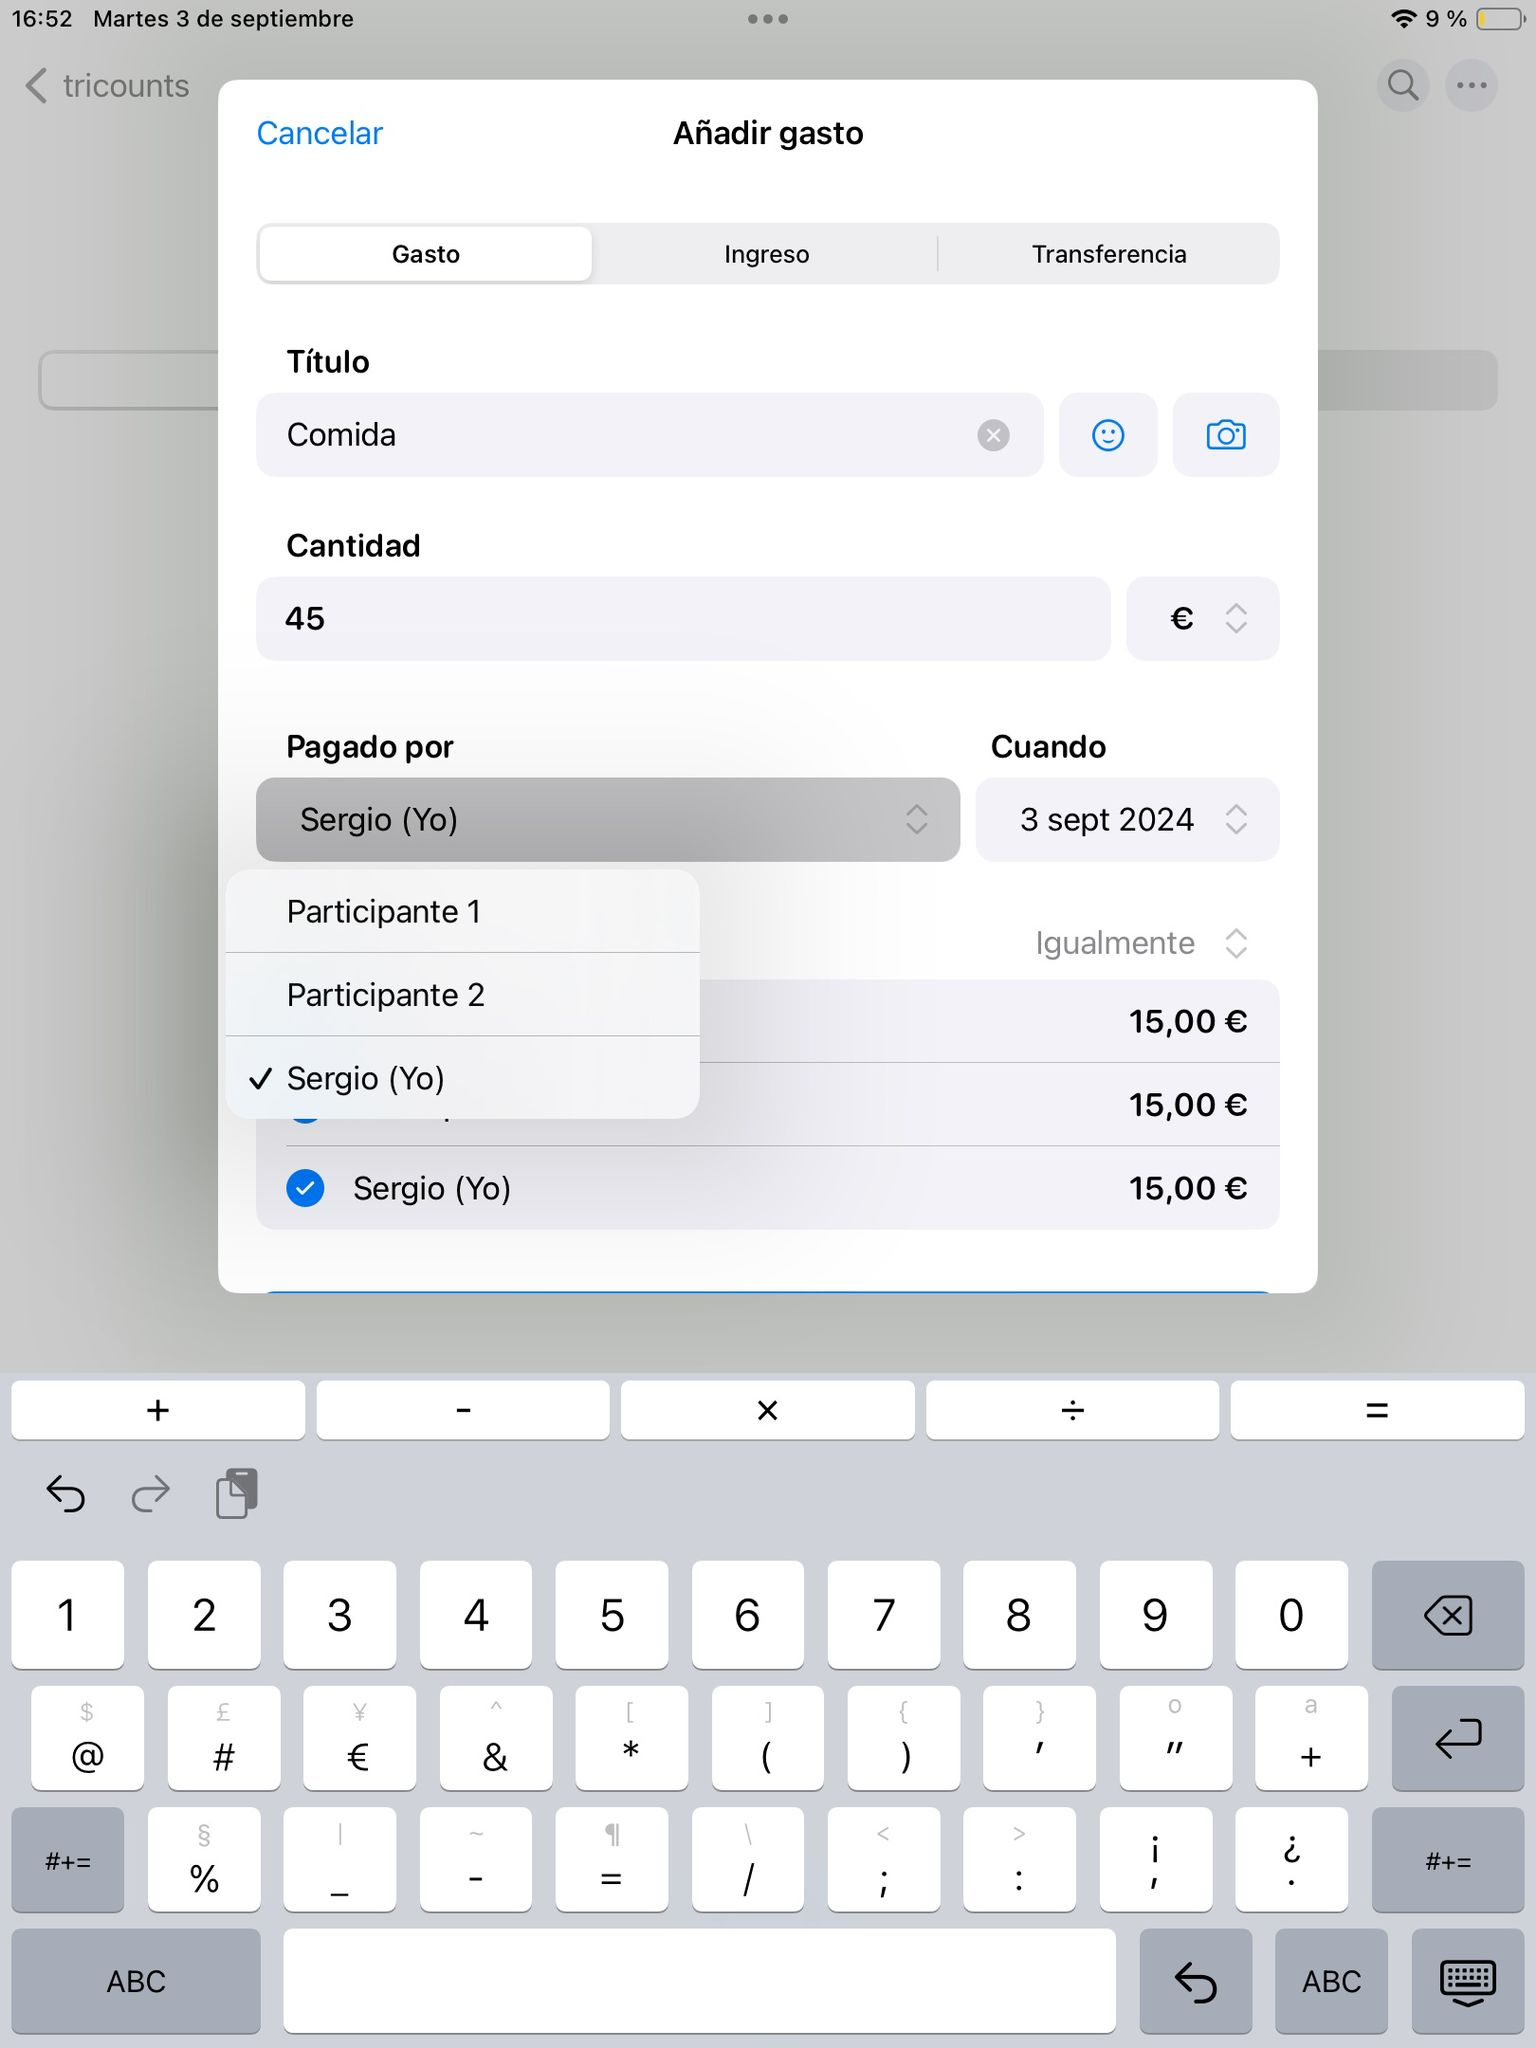
\includegraphics[width=\textwidth]{../capitulos/img/participantes.jpg}
        \caption{Añadir un gasto.}
        \label{participantes}
    \end{minipage}
    \hfill
    \begin{minipage}{0.45\textwidth}
        \centering
        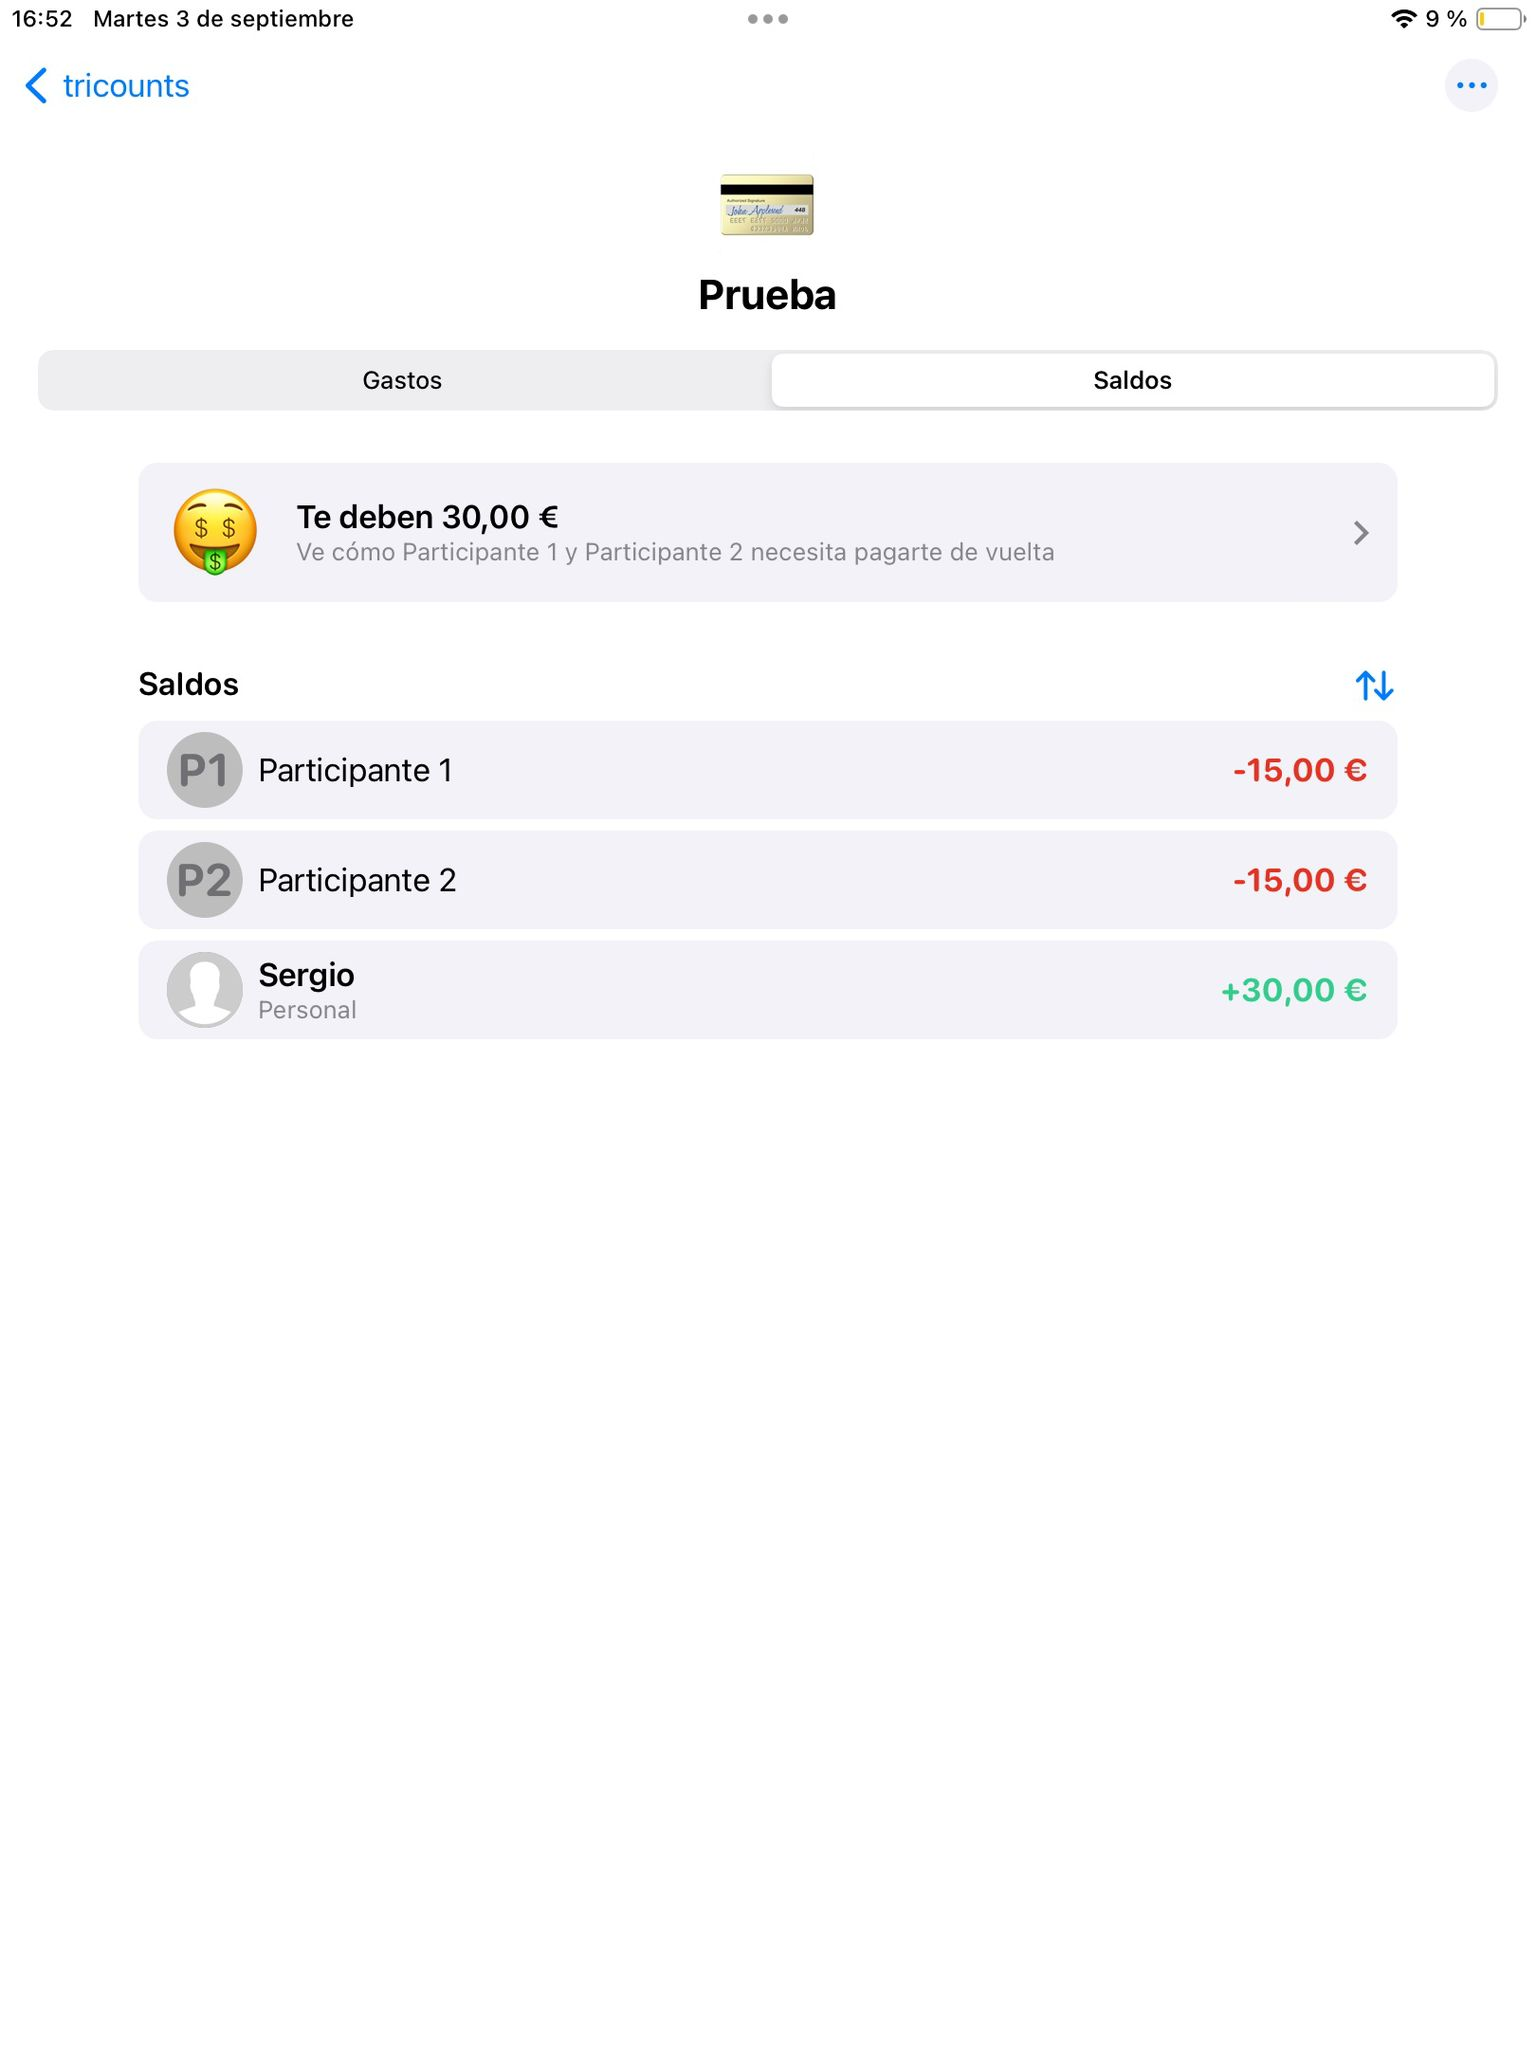
\includegraphics[width=\textwidth]{../capitulos/img/gastos.jpg}
        \caption{Resumen de los gastos y deudas.}
        \label{resumen}
    \end{minipage}
\end{figure}

Con esto ya tendríamos una idea de cómo funciona la aplicación, aunque hay muchas más funcionalidades que se pueden
realizar. 

\subsubsection{Calificación}
\label{subsec:calificacion}
En la tienda oficial de Android (\textit{Google Play}) la aplicación tiene una calificación de 4.8/5 estrellas y cuenta con más de 
10 millones de descargas y en la tienda oficial de Apple (\textit{App Store}) tiene una calificación de 4.7/5 estrellas. La mayoría de comentarios
son positivos y destacan la facilidad de uso y la utilidad de la aplicación.


\subsection{Todoist}
\label{sec:todoist}
Todoist es una aplicación de gestión de tareas y proyectos que ayuda a los usuarios a organizar sus actividades de manera diaria. 
Es ampliamente utilizada tanto por personas como por equipos, debido a su flexibilidad, interfaz intuitiva y capacidad para gestionar
desde simples listas de tareas hasta proyectos complejos. Está disponible para Android, iOS, Windows, Mac y la web.

\subsubsection{Funciones Principales}
\label{subsec:funciones_todoist}

\begin{enumerate}
    \item \textbf{Gestión de Tareas}
    \begin{enumerate}
        \item Añadir Tareas. Pueden crear tareas rápidamente. Cada tarea puede tener un título, una descripción y se puede asignar un proyecto o etiqueta para mantener todo organizado.
        \item Fechas de Vencimiento y Recordatorios. Se puede establecer una fechas límites para las tareas, además de recordatorios específicos, lo que ayuda a asegurarse de que las tareas se hagan a tiempo.
        \item Tareas Recurrentes. Si hay tareas que se repiten, se pueden configurar como tareas recurrentes. 
    \end{enumerate}
    \item \textbf{Proyectos y Subtareas}: 
    \begin{enumerate}
        \item Proyectos. Permite organizar las tareas dentro de proyectos. Los proyectos son carpetas donde se agrupan las tareas relacionadas con un objetivo o área específica.
        \item Subtareas. Para tareas más complejas, pueden descomponerlas en subtareas, permitiendo gestionar pasos más pequeños. 
    \end{enumerate}
    \item \textbf{Etiquetas y Filtros}
    \begin{enumerate}
        \item Etiquetas. Permiten agrupar tareas de diferentes proyectos a través de características comunes-
        \item Filtros. Permite crear vistas personalizadas de las tareas, según criterios como fechas, etiquetas, etc.
    \end{enumerate}
    \item \textbf{Prioridades}. Permite asignar niveles de prioridad a cada tarea, de 1 a 4
    \item \textbf {Colaboración y Gestión de Equipos}
    \begin{enumerate}
        \item Asignar Tareas. En proyectos compartidos, puedes asignar tareas a otros miembros del equipo, facilitando la colaboración en proyectos grupales. 
        \item Comentarios y Archivos. Los usuarios pueden añadir comentarios.
        \item Compartir Proyectos. Puedes compartir proyectos con otros usuarios, lo que permite que todos los miembros vean, añadan o editen tareas dentro de ese proyecto.
    \end{enumerate}
    \item \textbf{Integraciones}. Se integra con una amplia gama de aplicaciones y servicios, como Google Calendar, Slack, Dropbox, etc.
\end{enumerate}

\subsubsection{Modo de Uso}
\label{subsec:uso_todoist}
Lo primero que tenemos que hacer la primera que entramos en la aplicación es registrarnos a través de las diferentes opciones 
que nos permite la aplicación (\textit{Figura \ref{registro}}). Una vez completado este paso nos permite elegir 
el ámbito en el planeas usar la aplicación (he elegido personal porque es la que más se ajusta a la aplicación que estamos buscando).
(\textit{Figura \ref{ambito}}). Hecho todo esto nos lleva a la pantalla principal donde nos muestra las tareas que vencen hoy, en este caso
no aparece ninguna porque aún no hemos añadido nada (\textit{Figura \ref{principal_todoist}}). Si le damos a añadir nos permite poner
una descripción a la tarea, una fecha de vencimiento, una etiqueta, una prioridad, etc. (\textit{Figura \ref{añadir_tarea}}). Una vez añadida
nos aparece la tarea en nuestra lista de tareas pendientes donde la podemos marcar como realiza o no realizada. (\textit{Figura \ref{tarea}}).
También tenemos otra pestaña donde nos muestra un calendario con las tareas que tenemos pendientes por dias, además de la 
tarea que hemos añadido, nos muestra tareas de ejemplo (\textit{Figura \ref{calendario}}). Por último, cabe añadir que la aplicación cuenta
con otra pestaña donde se puede buscar tareas y otra para explorar ya que podemos tener tareas en diferentes bandejas.

\begin{figure}[ht]
    \centering
    \begin{minipage}{0.45\textwidth}
        \centering
        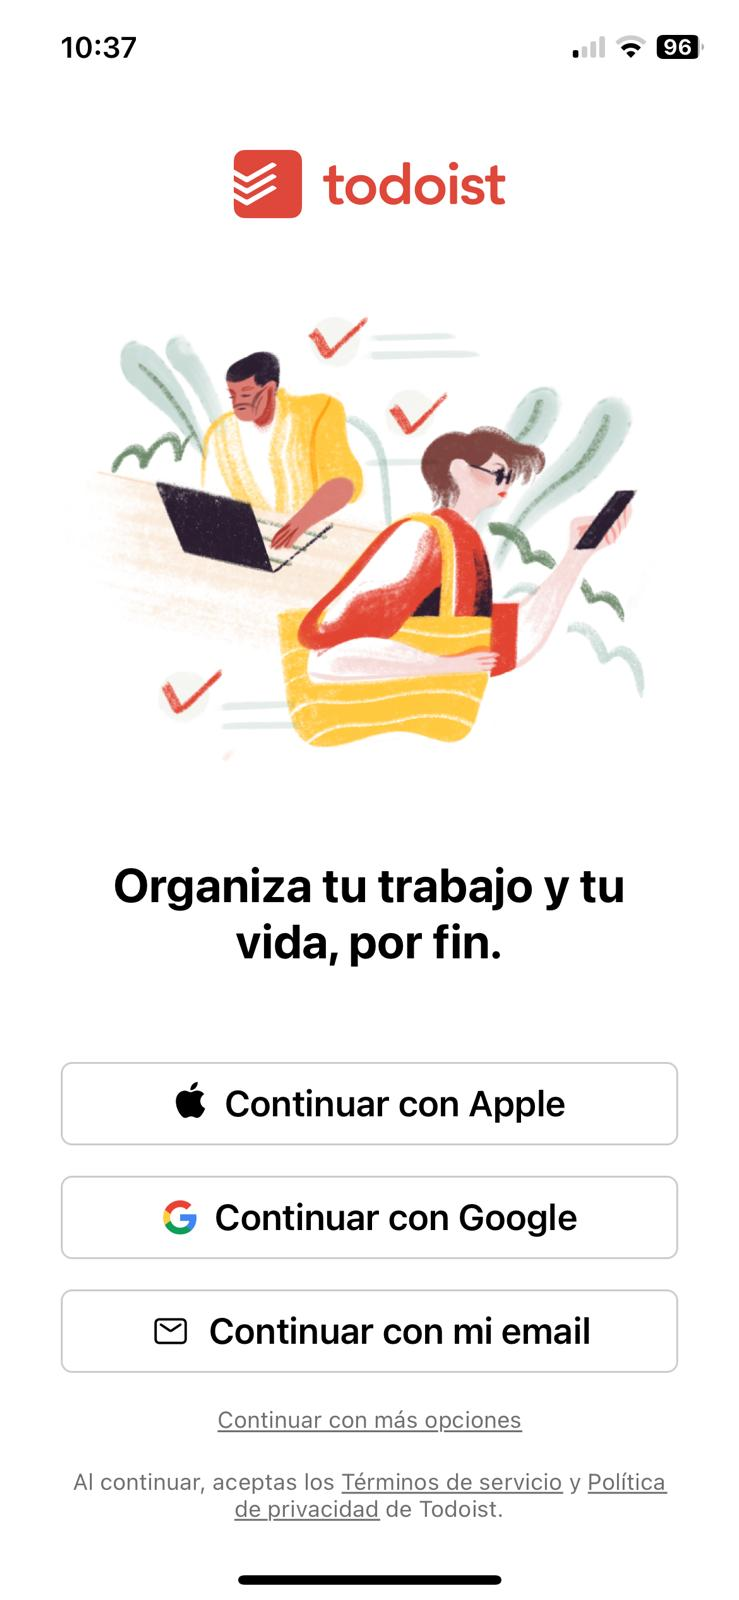
\includegraphics[width=\textwidth]{../capitulos/img/registro_todoist.jpg}
        \caption{Pantalla de registro.}
        \label{registro}
    \end{minipage}
    \hfill
    \begin{minipage}{0.45\textwidth}
        \centering
        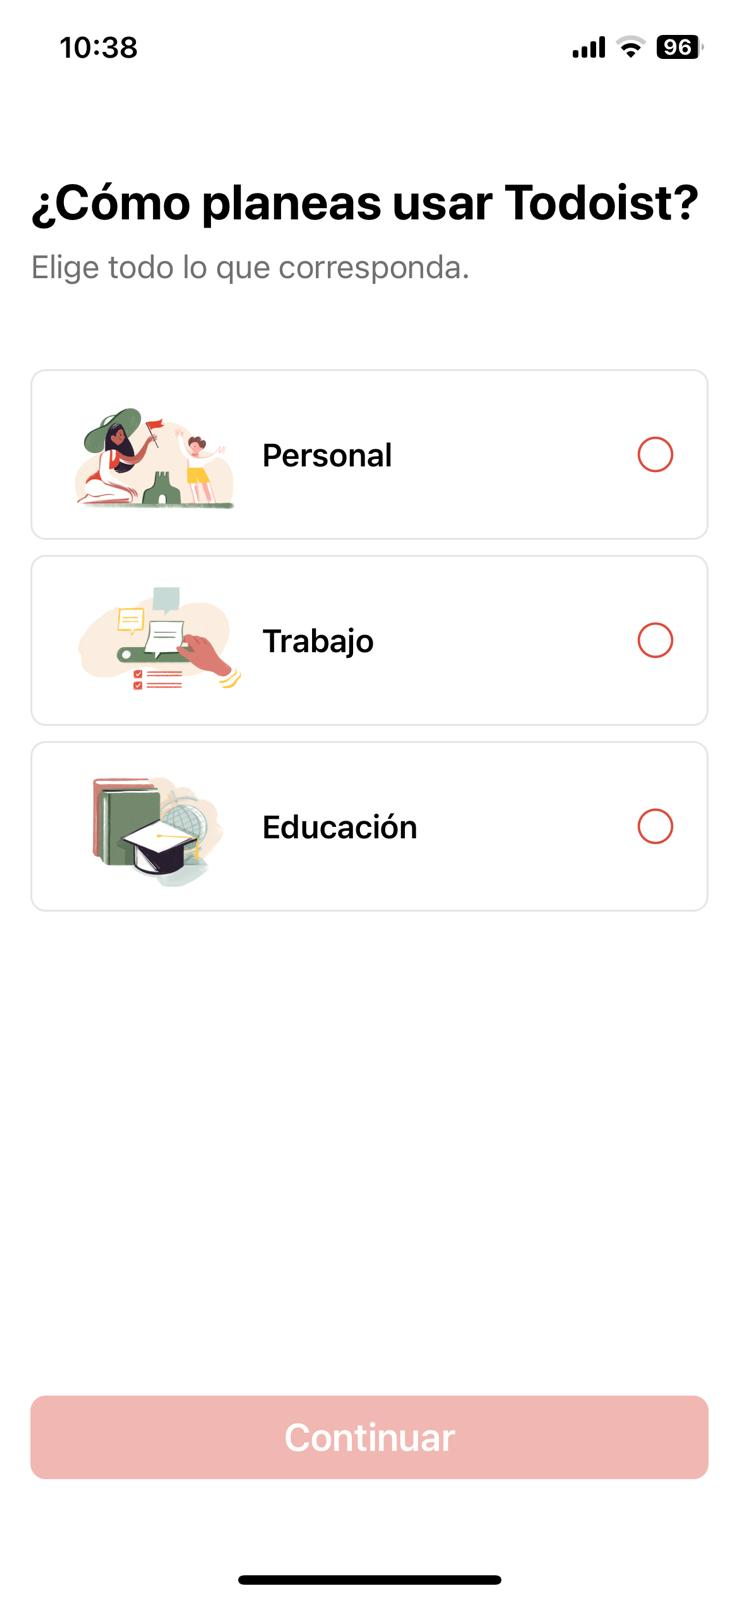
\includegraphics[width=\textwidth]{../capitulos/img/ambito_todoist.jpg}
        \caption{Elegir el ámbito de la aplicación.}
        \label{ambito}
    \end{minipage}
\end{figure}

\begin{figure}[ht]
    \centering
    \begin{minipage}{0.45\textwidth}
        \centering
        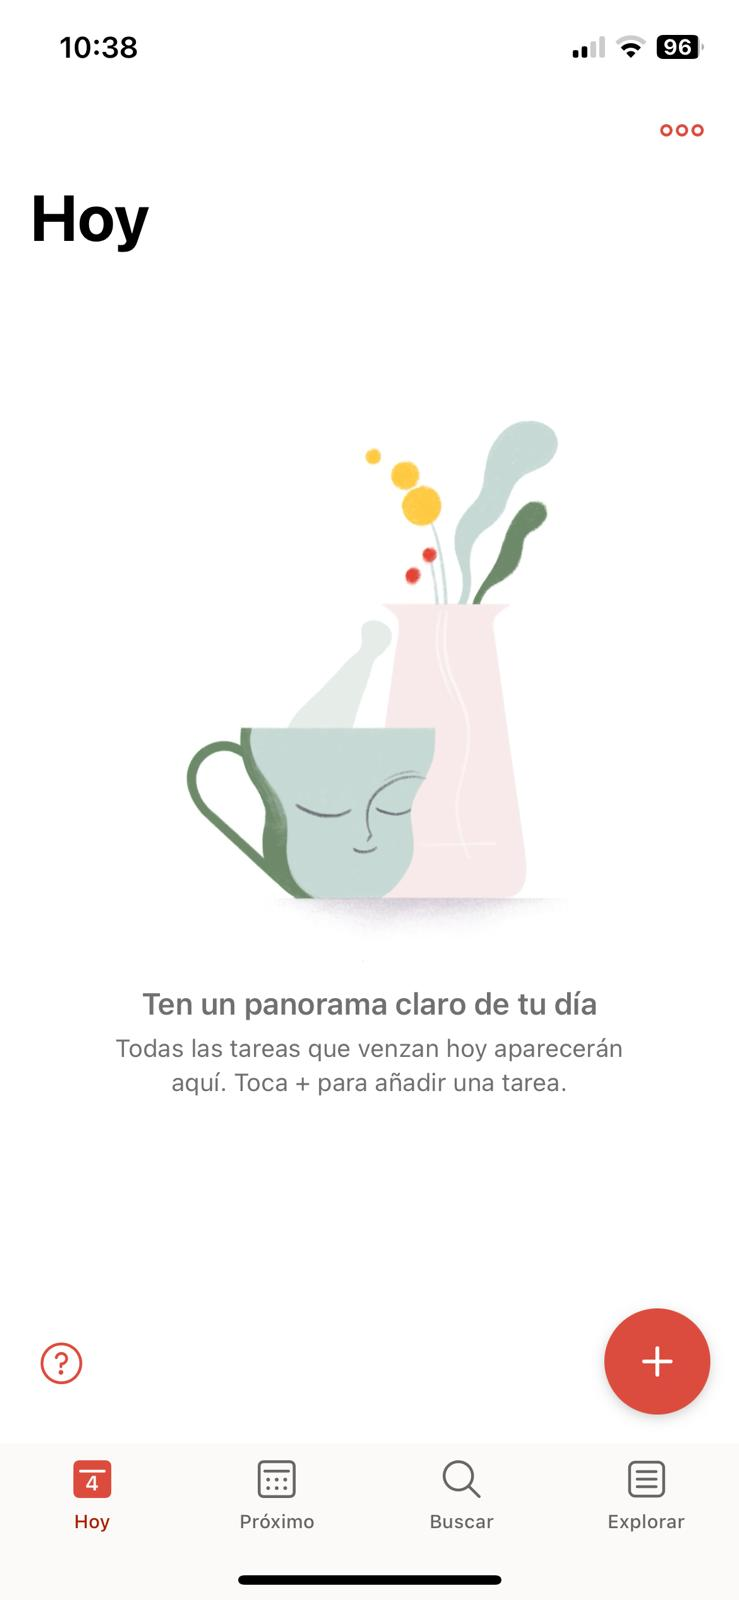
\includegraphics[width=\textwidth]{../capitulos/img/principal_todoist.jpg}
        \caption{Pantalla principal.}
        \label{principal_todoist}
    \end{minipage}
    \hfill
    \begin{minipage}{0.45\textwidth}
        \centering
        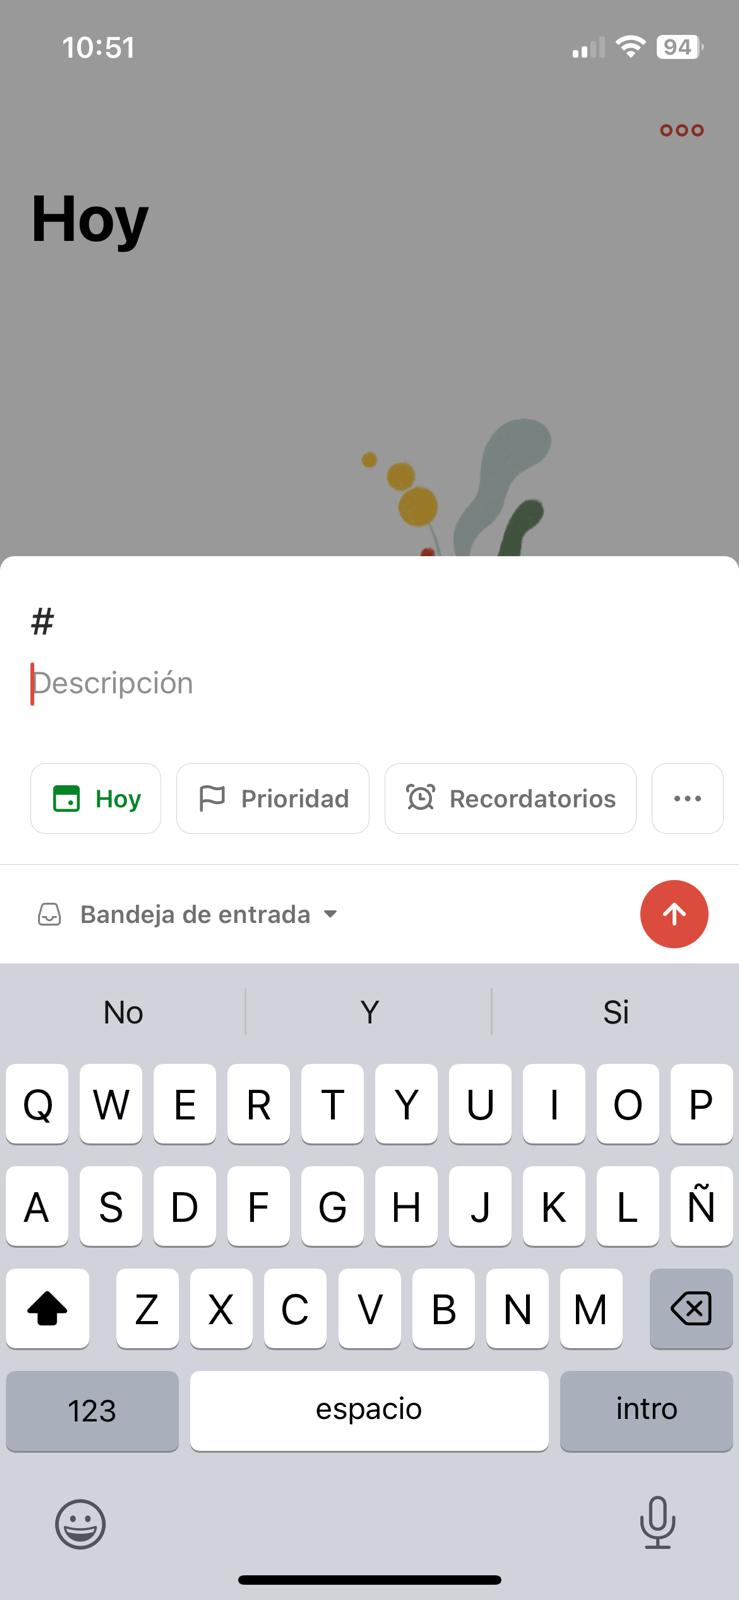
\includegraphics[width=\textwidth]{../capitulos/img/añadir_todoist.jpg}
        \caption{Añadir una tarea.}
        \label{añadir_tarea}
    \end{minipage}
\end{figure}

\begin{figure}[ht]
    \centering
    \begin{minipage}{0.45\textwidth}
        \centering
        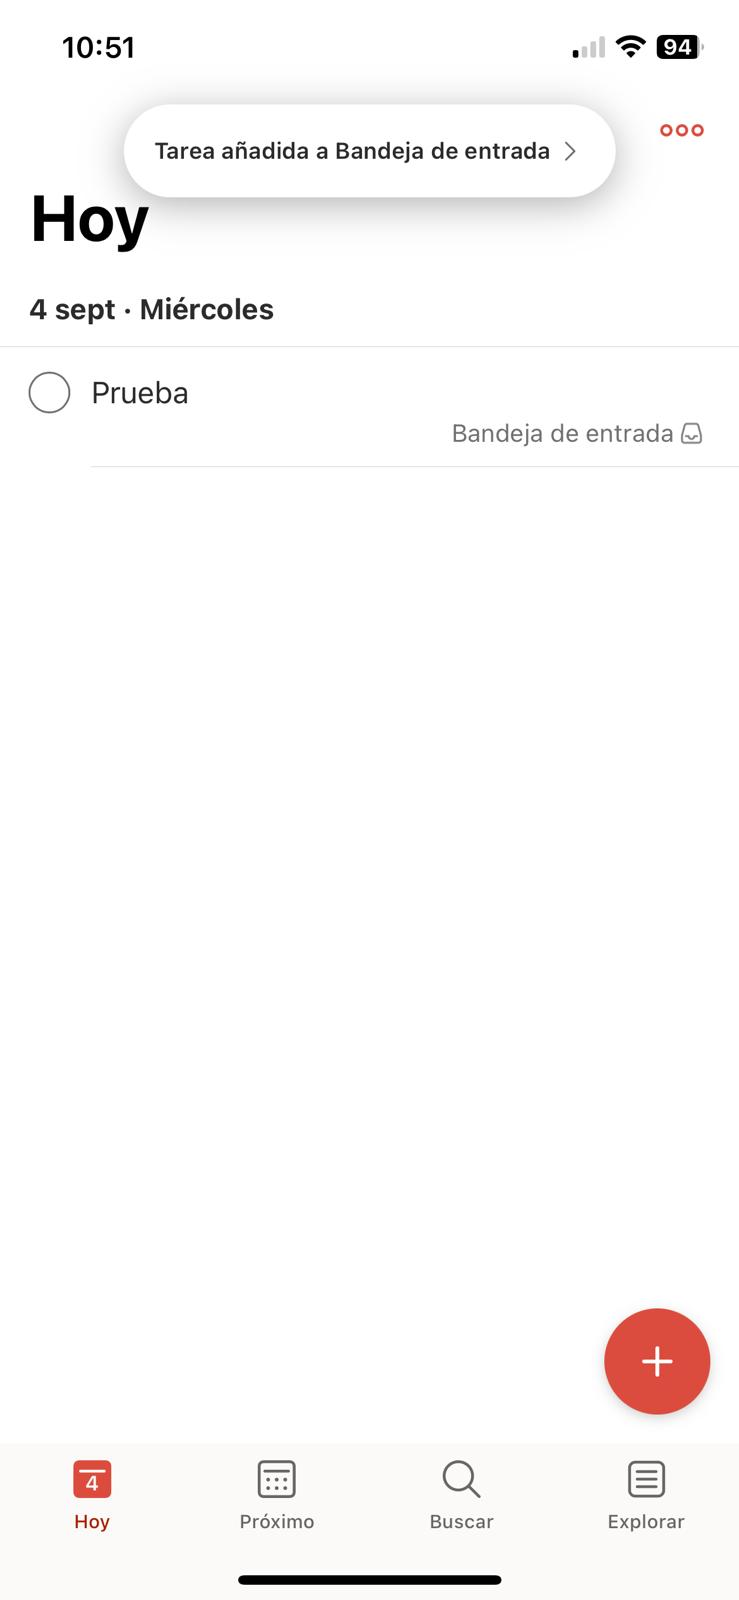
\includegraphics[width=\textwidth]{../capitulos/img/tarea_todoist.jpg}
        \caption{Pantalla con la tarea añadida.}
        \label{tarea}
    \end{minipage}
    \hfill
    \begin{minipage}{0.45\textwidth}
        \centering
        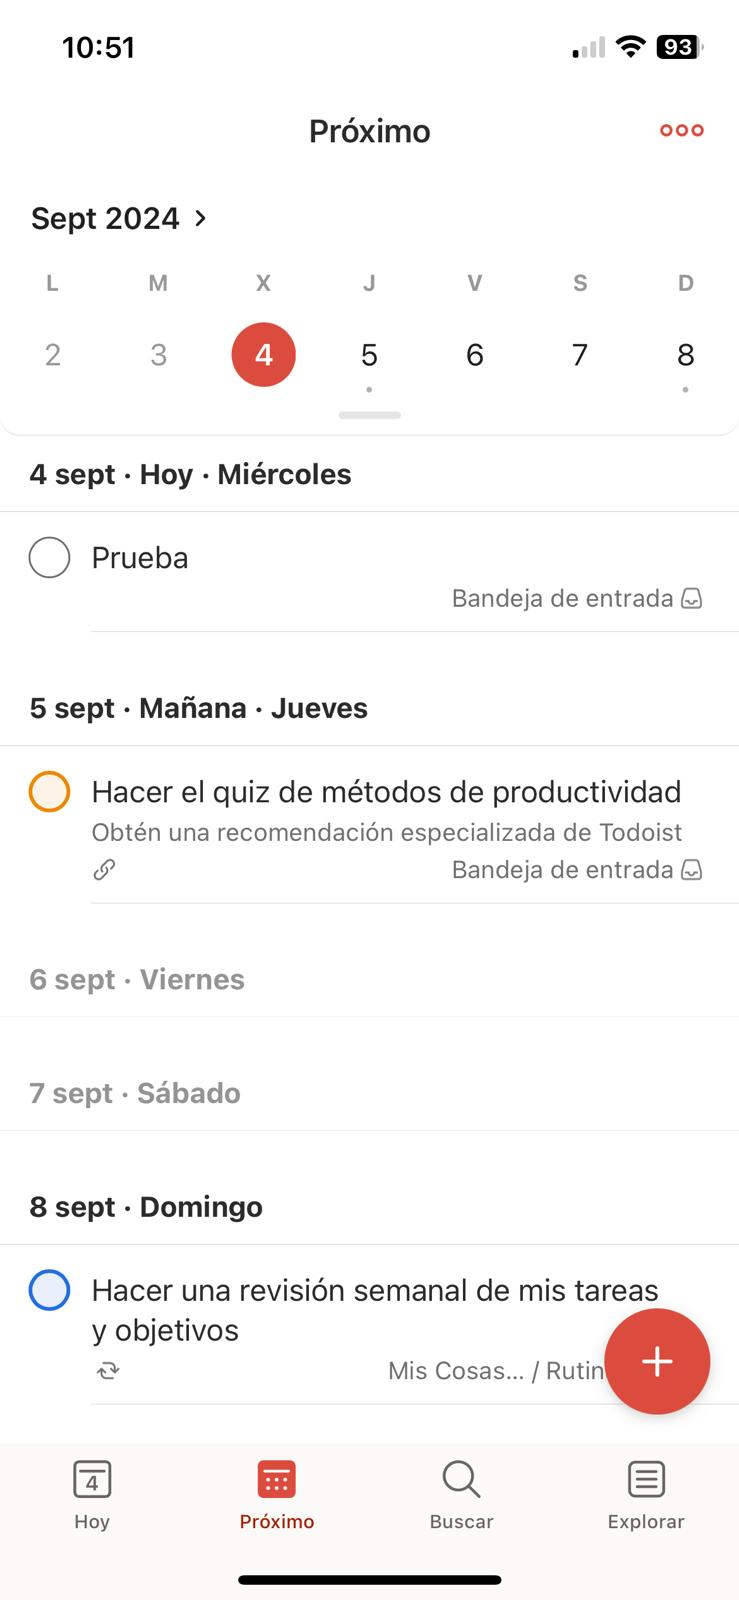
\includegraphics[width=\textwidth]{../capitulos/img/calendario_todoist.jpg}
        \caption{Calendario de tareas.}
        \label{calendario}
    \end{minipage}
\end{figure}

\subsubsection{Calificación}
\label{subsec:calificacion_todoist}
En la tienda oficial de Android (\textit{Google Play}) la aplicación tiene una calificación de 4.5/5 estrellas y cuenta con más de
10 millones de descargas y en la tienda oficial de Apple (\textit{App Store}) tiene una calificación de 4.7/5 estrellas. La mayoría de comentarios
son positivos y destacan la facilidad de uso y la utilidad de la aplicación. La versión de pago tiene un coste de 4.99\texteuro/mes o 47.99\texteuro/año.

\subsection{MeToca}
\label{sec:metoca}
Es una aplicación desarrollada por el gobierno de España con el objetivo de facilitar la organización de tareas del hogar
de manera equitativa y eficiente. Es una iniciativa para promover la corresponsabilidad en el hogar, asegurando que las
responsabilidades domésticas sean distruidas de manera justa entre todos los miembros de la familia. Es gratuita y 
en un principio estaba disponible para Android e iOS, pero en la actualidad solo está disponible para Android.
\subsubsection{Funciones Principales}

\begin{enumerate}
    \item \textbf{Gestión de Tareas del Hogar}
    \begin{enumerate}
        \item Asignación de tareas. Permite asignar tareas a cada miembro del hogar. Las tareas pueden ser de cualquier tipo
        \item Calendario y Recordatorios. Incluye un calendario integrado donde se pueden programar las tareas frecuentes o únicas.
        Además envía recordatorios en caso de no hacerlas a tiempo.
    \end{enumerate}
    \item \textbf{Seguimiento y Cumplimiento}
    \begin{enumerate}
        \item Registro de Tareas Completadas. Cada usuario puede marcar sus tareas completadas y así poder llevar unn control del cumplimiento de responsabilidades.
        \item Estadísticas de Participación. Genera informes y estadísticas sobre cómo se están distribuyendo las tareas y si se están cumpliendo.
    \end{enumerate}
    \item \textbf{Distribución Equitativa}
    \begin{enumerate}
        \item Corresponsabilidad. Fomenta la corresponsabilidad en el hogar a través de la visualización 
        y el seguimiento de tareas todos los miembros pueden ver si las responsabilidades se están distribuyendo de manera equitativa.
    \end{enumerate}
    \item \textbf{Soporte para diferentes tipos de hogares}
    \begin{enumerate}
        \item Adaptabilidad. Está diseñada para ser inclusiva y adapatable para cualquier tipo de hogar o de familia
        \end{enumerate}
\end{enumerate}

\subsubsection{Modo de Uso}
\label{subsec:uso_metoca}
En este caso no he podido probar la aplicación ya que no está disponible para iOS.

\subsubsection{Calificación}
\label{subsec:calificacion_metoca}
En la tienda oficial de Android (\textit{Google Play}) la aplicación tiene una calificación de 1.6/5 estrellas,
con apenas más de 10.000 descargas, aunque los creadores aseguran que tienen muchisimas funcionalidades la mayoría de comentarios
aseguran que no les resulta muy útil.

\subsection{Cozi Family Organizer}
\label{sec:cozi}
Es una aplicación diseñada para ayudar a las familias a organizar y gestionar sus actividades diarias para auidar a las familias a organizar y 
gestionar sus actividades de manera colaborativa. Cozi se enfoca en la simplicidad y en proporcionar funciones esenciales para coordinar 
las actividades de varios miembros de una familia ocupada. Está disponible para Android, iOS y la web. Dispone de una versión 
gratuita que incluye la mayoría de las funcionalidades principales y una versión de pago con funciones adicionales.

\subsubsection{Funciones Principales}
\label{subsec:funciones_cozi}

\begin{enumerate}
    \item \textbf{Calendario Familiar}
    \begin{enumerate}
        \item Calendario Unificado. El calendario de Cozi hace que todos los miembros de la familia tengan acceso a un calendario compartido. 
        Cada miembro de la familia tiene un color asignado, lo que facilita ver quién tiene cada actividad y cuando tiene que hacerla.
        \item Eventos y Recordatorios. Se pueden añadir eventos y establecer recordatorios para asegurar que madie olvide compromisos importantes, cómo
        citas médicas, actividades escolares o eventos familiares.
        \item Notificaciones. La aplicación envía notificaciones a los miembros de la familia sobre los eventos próximos, asegurando que todo estén informados de los planes.
    \end{enumerate}
    \item \textbf{Lista de Compras Compartidas}
    \begin{enumerate}
        \item Lista de Compras Colaborativas. Permite crear y compartir listas de compras entre todos los miembro de la familia, 
        lo que permite que varias personas puedan contribuir a la lista y cualquier miembro puede marcar articulos que ya se han comprado. 
        \item Actualizaciones en Tiempo Real. La lista de compras se actualiza en tiempo real, lo que significa que cualquier cambio que se haga se refleja inmediatamente en todos los dispositivos.
        \item Organización por Tienda. Las listas pueden organizarse por tipo de tienda o categoría.
    \end{enumerate}
    \item \textbf{Listas de Tareas}
    \begin{enumerate}
        \item Tareas Pendientes. Permite crear listas para proyectos domésticos, responsabilidades diarias o cualquier tipo de actividades pendientes
        \item Marcar Completadas. Los usuarios pueden marcarla como hecha, lo que ayuda a mantener un seguimiento claro de lo que se ha logrado
    \end{enumerate}
    \item \textbf{Planificación de Comidas}
    \begin{enumerate}
        \item Organizador de Menús. Facilita organizar las comidas con antelación y evita el estrés diario de decidir qué cocinar. 
        \item Recetas Integradas. Puedes guardar y organizar recetas directamente en la aplicación y con solo un clic. 
        \item Sincronización con el calendario. Los menús planificados pueden sincronizarse con el calendario para que toda la familia lo vea. 
    \end{enumerate}
    \item \textbf{Diario Familiar}. Es una función donde los miembros pueden registrar eventos o recuerdos importantes, como fotos y notas sobre actividades familiares. 
    Además se puede compartir con otro familiares y amigos.
\end{enumerate}

\subsubsection{Modo de Uso}
\label{subsec:uso_cozi}
Después de descargar e instalar esta aplicación, lo primero que nos muestras es una pantalla de registro/inicio de sesión (\textit{Figura \ref{registro_cozi}}).
donde nos pide un nombre, el correo electrónico y una contraseña. Después de crear nuestra cuenta nos muestra una pantalla donde nos pide 
el nombre de nuestra familia y los miembros que la componen (\textit{Figura \ref{familia_cozi}}). Después de esto nos permite añadir un evento al calendario, con
un nombre, la fecha, quién la tiene que realizar, si se repite o no y cúando queremos que nos lo recuerde (\textit{Figura \ref{evento_cozi}}). Una vez completado este 
paso nos muestra el un calendario con todas las tareas que tenemos pendientes (\textit{Figura \ref{calendario_cozi}}). Si nos vamos a la pestaña de "List"
nos muestras todas las listas de compras o de cosas que hacer ya que están divididas en dos pestañas, en la (\textit{Figura \ref{listas}}) podemos ver un ejemplo de lista 
de la compra con un árticulo añadido a una de ellas. Otra de las pestañas que nos ofrece la aplicación es la de "Recetas" donde nos muestra recetas de cocina y además nos deja 
añadir más recetas a través de una url de la receta encontrada (\textit{Figura \ref{recetas}}). Por último, la pestaña final es la de "Familia" donde nos permite configurar información sobre la familia, por ejemplo, 
añadir una foto de perfil o añadir a un miembro más a la familia. 

\begin{figure}[ht]
    \centering
    \begin{minipage}{0.45\textwidth}
        \centering
        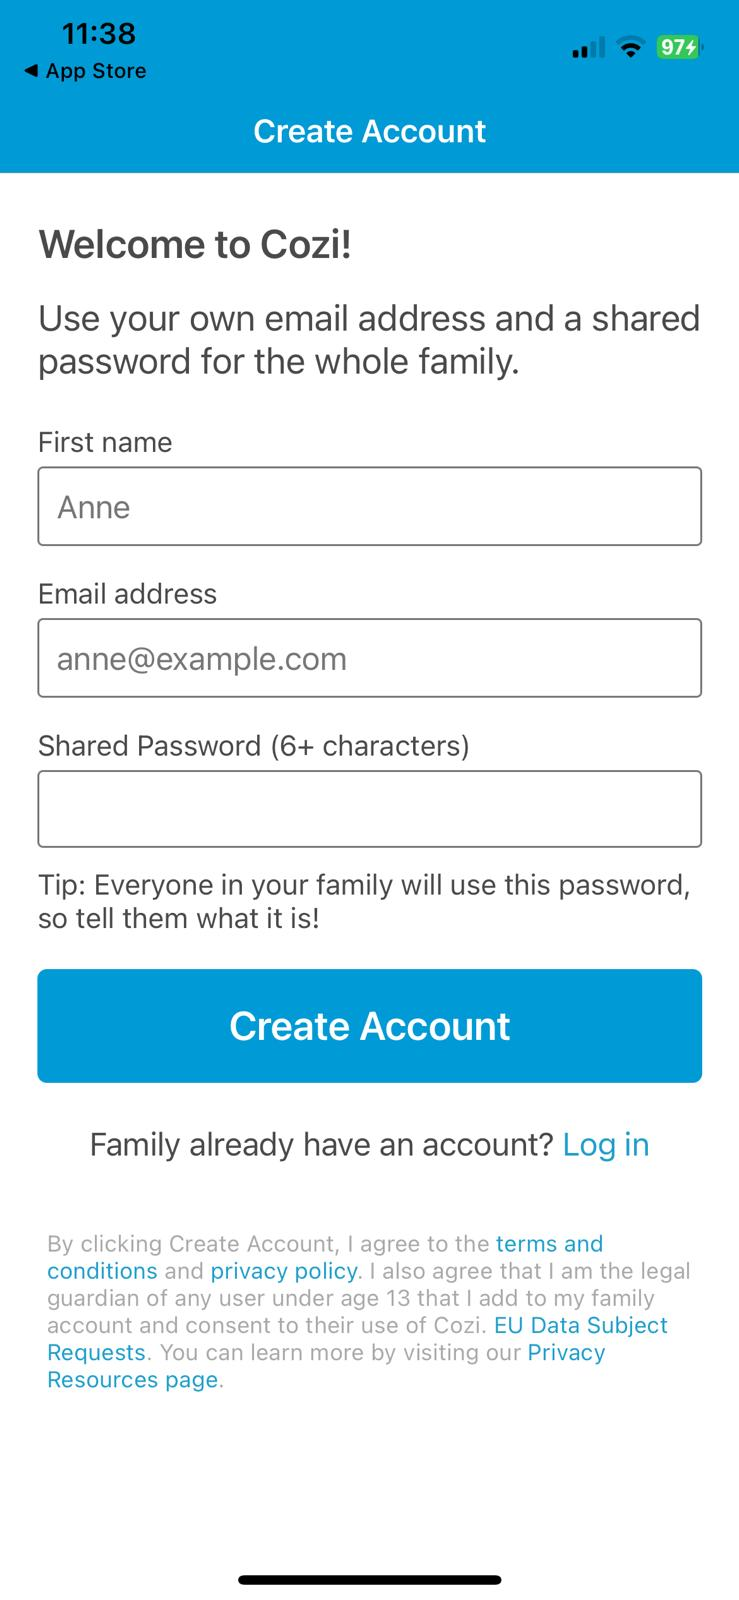
\includegraphics[width=\textwidth]{../capitulos/img/registro_cozi.jpg}
        \caption{Registro.}
        \label{registro_cozi}
    \end{minipage}
    \hfill
    \begin{minipage}{0.45\textwidth}
        \centering
        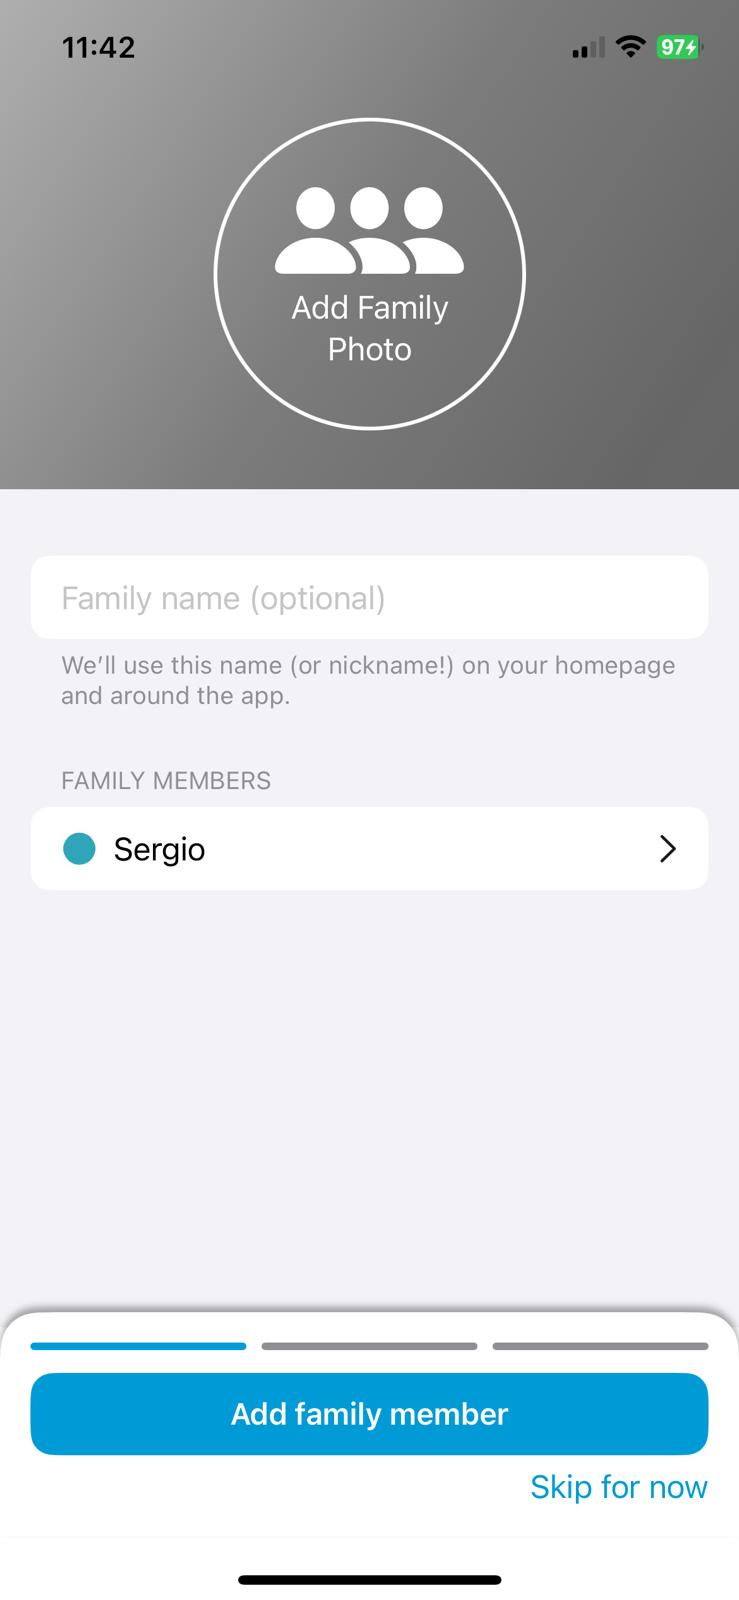
\includegraphics[width=\textwidth]{../capitulos/img/familia_cozi.jpg}
        \caption{Crear una familia.}
        \label{familia_cozi}
    \end{minipage}
\end{figure}

\begin{figure}[ht]

    \begin{minipage}{0.45\textwidth}
        \centering
        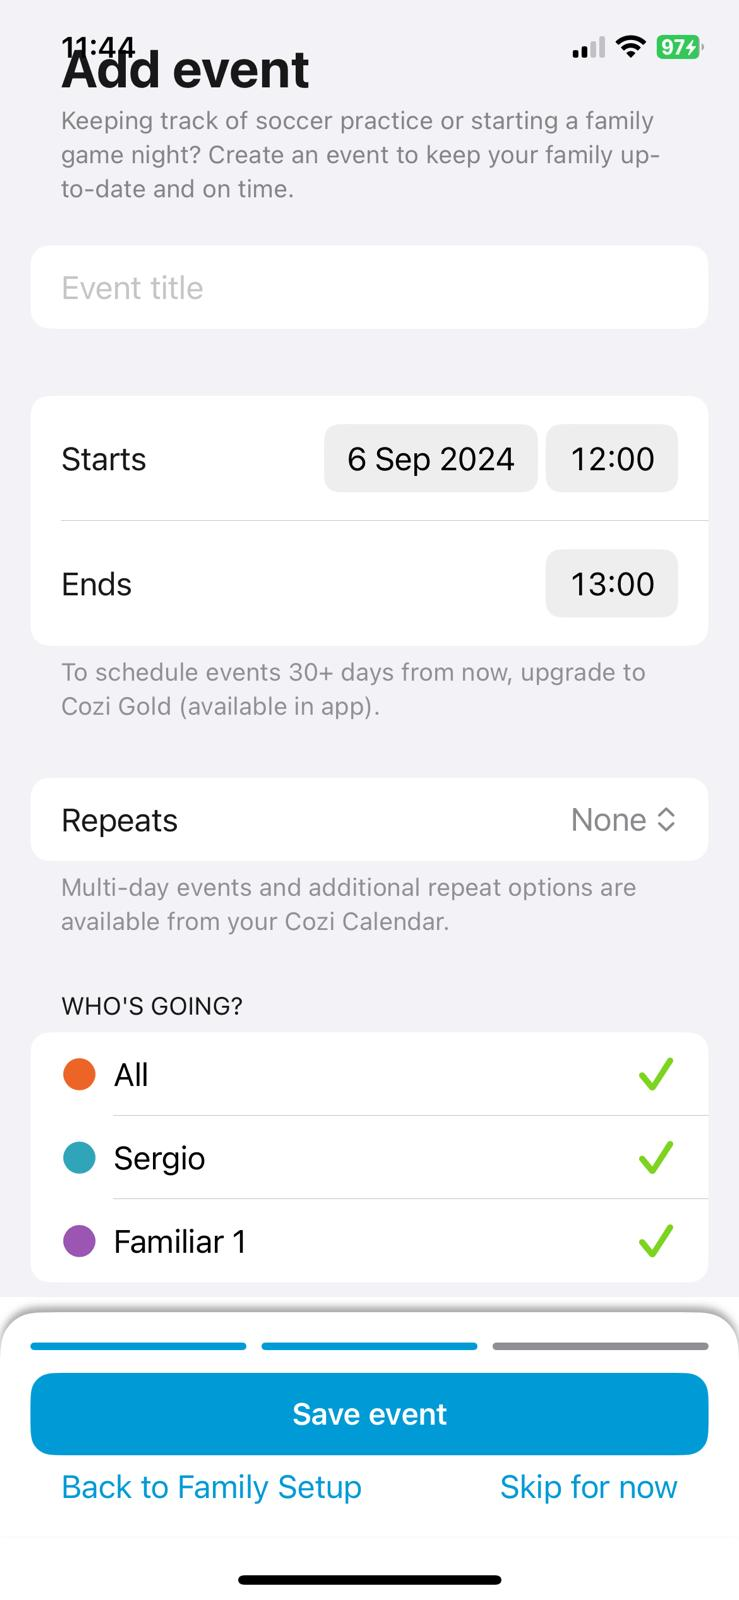
\includegraphics[width=\textwidth]{../capitulos/img/evento_cozi.jpg}
        \caption{Añadir un evento.}
        \label{evento_cozi}
    \end{minipage}
    \hfill
    \begin{minipage}{0.45\textwidth}
        \centering
        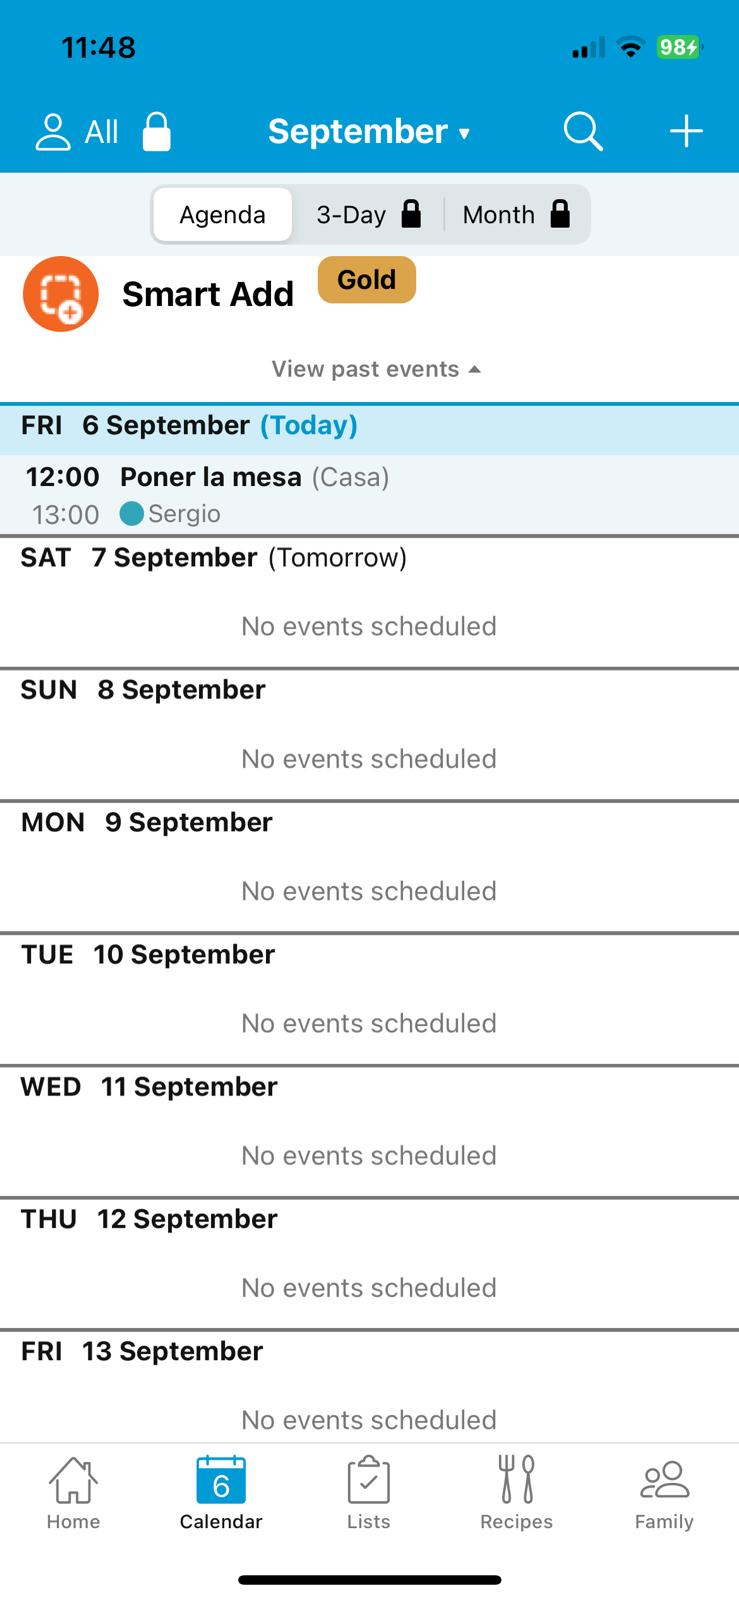
\includegraphics[width=\textwidth]{../capitulos/img/calendario_cozi.jpg}
        \caption{Calendario.}
        \label{calendario_cozi}
    \end{minipage}
\end{figure}

\begin{figure}[ht]

    \begin{minipage}{0.45\textwidth}
        \centering
        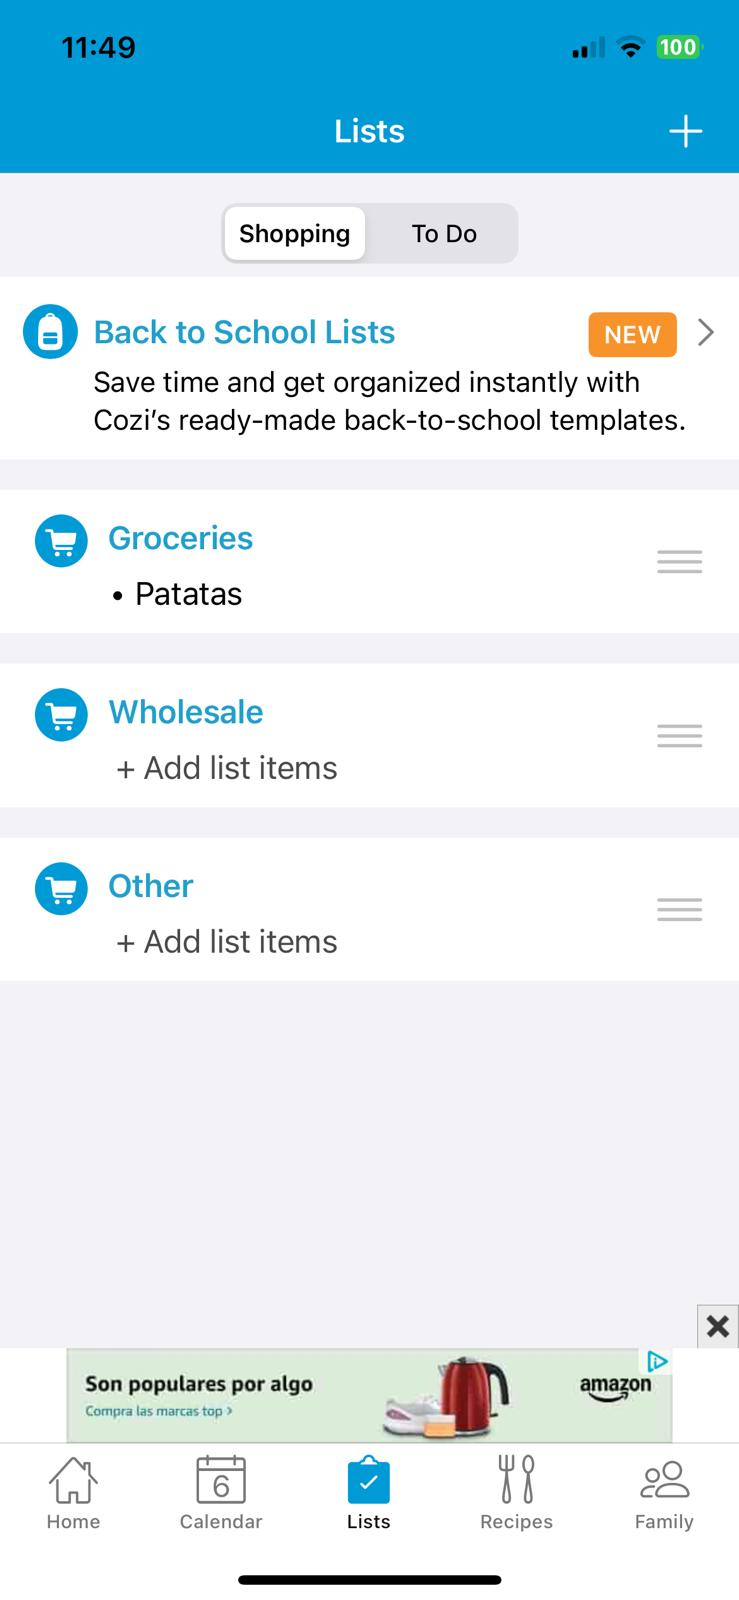
\includegraphics[width=\textwidth]{../capitulos/img/listas_cozi.jpg}
        \caption{Listas de la compra.}
        \label{listas}
    \end{minipage}
    \hfill
    \begin{minipage}{0.45\textwidth}
        \centering
        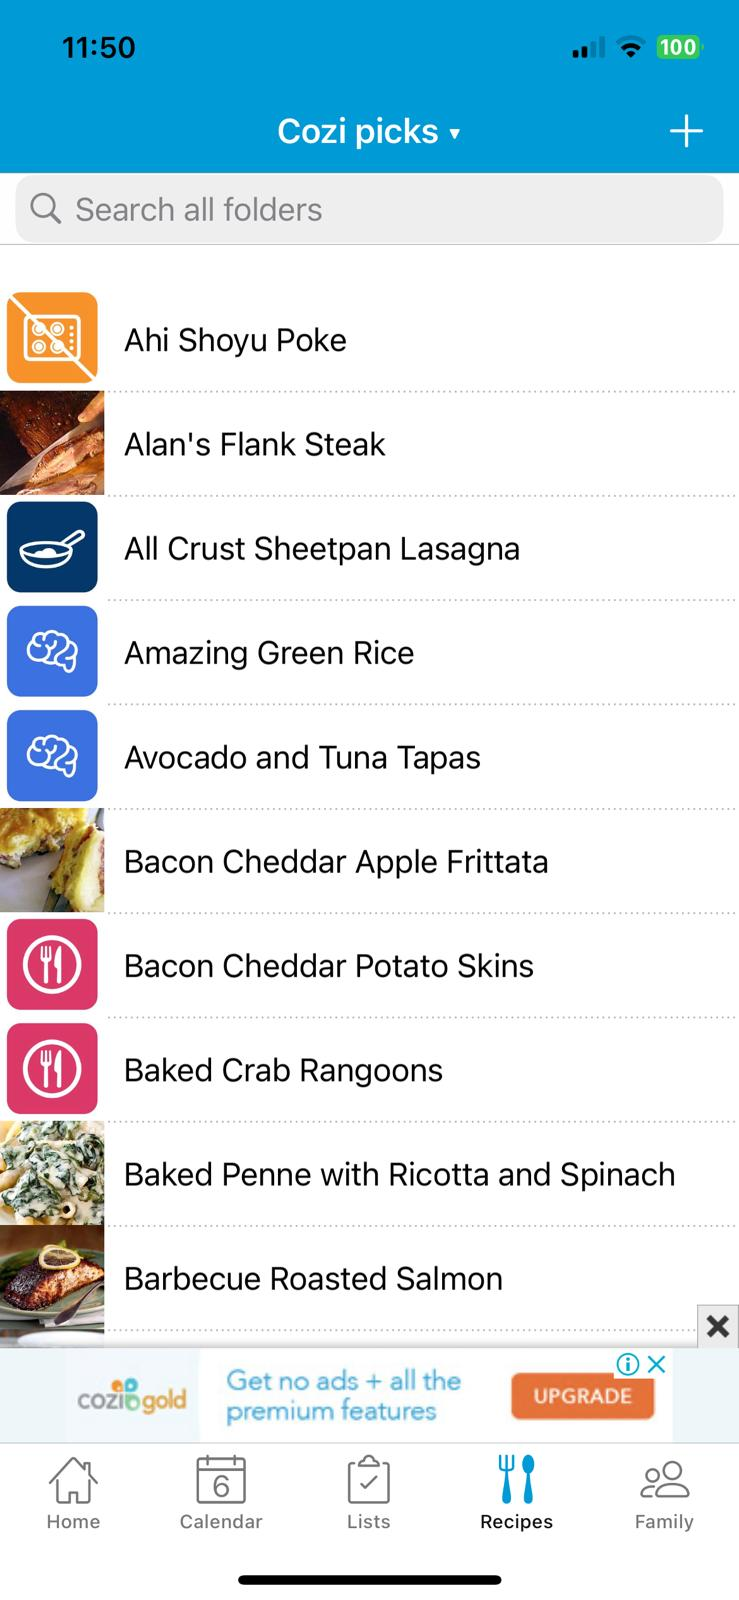
\includegraphics[width=\textwidth]{../capitulos/img/recetas_cozi.jpg}
        \caption{Recetas.}
        \label{recetas}
    \end{minipage}
\end{figure}




\subsubsection{Calificación}
\label{subsec:calificacion_cozi}
En la tienda oficial de Android (\textit{Google Play}) la aplicación tiene una calificación de 4.1/5 estrellas y cuenta con más de 5 millones de descargar. 
En la tienda oficial de Apple (\textit{App Store}) tiene una calificación de 4.8/5 estrellas. La mayoría de comentarios son positivos y destacan la facilidad de uso y la utilidad de la aplicación.
Por lo que he podido observar la página esta completamente en inglés. 

\subsection{OurHome}
\label{sec:ourhome}
Es una aplicación que ayuda a familias a organizar y gestionar tareas, compras y responsabilidades diarias de manera colaborativa. 
Está diseñada para facilitar la administración de tareas en el hogar y fomentar la cooperación familiar mediante asignación de tareas, 
el seguimiento de recompensas y la planificación de compras. 

\subsubsection{Funciones Principales}
\label{subsec:funciones_ourhome}

\begin{enumerate}
    \item  \textbf{Asignación de Tareas}. Permite asignar y crear tareas a los miembros de la familia, definiendo la frecuencia y quien debe hacer cada tarea y en qué plazo.
    Además incluye un sistema de recompensas basado en puntos, donde los miembros ganan puntos al completar tareas.
    \item \textbf{Lista de Compra Compartida}. Incluye una lista de compras integrada que puede ser gestionada por cualquier miembro de la familia. Permite categorizar artículos y marcarlos como comprados.
    \item \textbf{Calendario Familiar}. Incluye un calendario compartido donde se pueden añadir eventos y recordatorios, donde cada miembro puede ver y agregar eventos.
    \item \textbf{Seguimiento de Objetivos}. Permite a los padres establecer objetivos específicos para los niños o cualquier miembro de la familia, cómo hábitos de estudio o rutinas diarias 
    \item \textbf{Sistema de notificaciones}. Los usuarios reciben notificaciones cuando se les asigna una tarea, se acerca la fecha límite o se actualiza la lista de compras.
\end{enumerate}

\subsubsection{Modo de Uso}
\label{subsec:uso_ourhome}
Si nos metemos desde la página web oficial de la aplicación, nos aparece un enlace para que la descarguemos en nuestro dispositivo iOS, 
sin embargo, en mi dispositivo iOS no me da la opción de instalarmela, por lo tanto, tras investigar, llegué a la conclusión de que la aplicación no 
está disponible para nuestra región.

\subsubsection{Calificación}
\label{subsec:calificacion_ourhome}
En la tienda oficial de Android (\textit{Google Play}) la aplicación tiene no tiene ningún tipo de calificación y solo cuanta con un poco más de 500 descargas. 
No aparece ningún tipo de comentario por lo tanto se deduce, que no es una aplicación muy popular. 


\subsection{Comparativa}
\label{sec:comparativa}

A continuación se muestra una tabla comparativa de las aplicaciones analizadas, donde se resumen las principales características y funcionalidades de cada una: 

\begin{table}[ht]
    \centering
    \resizebox{\textwidth}{!}{%
    \begin{tabular}{|c|c|c|c|c|c|}
        \hline
        & \textbf{Tricount} & \textbf{Todoist} & \textbf{MeToca} & \textbf{Cozi Family Organizer} & \textbf{OurHome} \\ \hline
        Plataforma & Android, iOS y web & Android, iOS, Windows, Mac y web & Android & Android, iOS y web & Android \\ \hline
        Coste & Grautito & Grautito y Pago & Gratuito & Grautuito y Pago & Gratuito \\ \hline
        Calificación Media  & 4.75 & 4.6 & 1.6  & 4,45 & -- \\ \hline
        Control de Gastos & \checkmark & -- & -- & -- & -- \\ \hline
        Gestión de Tareas & -- & \checkmark & \checkmark & \checkmark & \checkmark \\ \hline
        Calendario & -- & \checkmark & -- & \checkmark & \checkmark \\ \hline
        Lista de Compras & -- & -- & -- & \checkmark & \checkmark \\ \hline
        Asignación de Tareas & -- & -- & \checkmark & \checkmark & \checkmark \\ \hline
        
      
    \end{tabular} %
    }

\end{table}

\newpage

\section{Estudio de la distribución del tiempo y gestión del hogar en entornos compartidos}

Un estudio del \textit{American Time Use Survey (ATUS)}, analiza la distribución del tiempo que las personas dedican a la administración del hogar
y cómo esta tarea se realiza en intervalos dispersos. Este estudio revela patrones en las actividades domésticas y ayuda a entender los 
desafío de coordinación y planificación en hogares donde las responsabilidades se dividen entre varias personas. El estudio muestra
que las tareas del hogar, como la limpieza, la preparación de comidas, la organización y la gestión de finanzas, tienden a realizarse en 
intervalos de tiempo que varían significativamente entre los distintos miembros del hogar. Esto es problemático en hogares compartidos, como 
los estudiantes o trabajadores, donde la disponibilidad de cada persona depende de su carga académica o laboral. La falta de tiempos fijos y 
la irregularidad en la dedicación a las tareas puede generar problemas de coordinación, ya que cada miembro tiene su propio horario, lo que impide
una rutina doméstica unificada.

Otro hallazgo importante de este estudio es que las tareas domésticas se realizan de manera inconsistente debido a limitaciones de tiempo y energía, especialmente
entre aquellos con empleos de tiempo completo o estudiante con cargas académicas pesadas. Esta incosistencia es común en los hogares compartidos,
donde la carga se divide entre varias personas sin un sistema claro de asignación de responsabilidades o seguimiento. Sin herramientas adecuadas
para la organización, es posible que algunas tareas queden sin realizar o que recaigan siempre en las mismas personas, generando frustración y posibles 
conflictos.

El estudio también resalta que, a medida que los individuos se ven cada vez más presionados por sus estudios o trabajos, tienden a posponer las tareas del hogar, lo cual se 
agrava en entornos de convivencia compartida. Este aplazamiento puede llevar a una acumulación de tareas, que a su vez aumenta el nivel de estrés de los residentes y genera tensiones en el hogar.

Por último, los resultados también sugieren que la organización efectiva del hogar es crucial para el bienestar de sus miembros. En el contexto de hogares compartidos,
el uso de herramientas de planificación o aplicaciones específicas podría mejorar significativamente la administración de tareas y reducir el 
estrés relacionado con el hogar \cite{american2022}.





\section{Estudio sobre los desafíos financieros en viviendas estudiantiles compartidas}
El estudio basado en datos de HUD, examina los desafíos financieros que enfrentan los estudiantes en viviendas compartidas. Uno de los hallazgos
principales de este estudio es que los contratos de arrendamiento de las viviendas a menudo requieren compromisos anuales. Los estudiantes deben 
seguir pagando el alquiler durante todo el año, incluso en períodos en que la vivienda está vacía, como los meses de verano. Este requisito genera una carga
financiera adicional, ya que los estudiantes deben encontrar formas de cubrir los pagos durante esos meses.

También señala que la organización de los gastos compartidos es una tarea compleja para los estudiantes. Dado que los contratos incluyen puede incluir 
diferentes servicios, la variación en las facturas mensuales añade dificultad al reparto equitativo de costes. Muchos estudiantes carecen de herramientas 
y sistemas de organización, lo que provoca confusión y conflictos en cuanto a las cantidades que cada miembro debe pagar. Esto puede ser 
díficil de gestionar cuando uno o varios de los residentes enfrentan problemas financieros, ya que retrasos o impagos afectan a todos los miembros del hogar.

Por último, este estudio también examina cómo las dificultades para gestionar los gastos afectan no solo la situación financiera de los estudiantes, 
sino también su bienestar general y rendimiento académico. La preocupación por la estabilidad financiera y la tensión asociada con la administración de los 
costos compartidos afectan a los estudiantes a nivel psicológico y académico, ya que deben dedicar su tiempo y energía a resolver estos problemas, lo que limita 
su concentración en los estudios. \cite{hud2022}

\newpage

\section{Legislación actual de protección de datos}

La \textbf{Ley de Protección de Datos} está diseñada para garantizar el derecho a la privacidad y 
la protección de los datos personales, evitando el uso indebido o la divulgación de la información 
personal de personas. En la Unión Europea, la normativa más relevante es el 
\textbf{Reglamento General de Protección de Datos (GDPR)}, que entró en vigor en 2018 y 
establece un estándar estricto para el manejo de datos en todos los países miembros, aplicando también 
a empresas fuera de la UE que traten datos de ciudadanos europeos. En España, esta ley se complementa con 
la \textbf{Ley Orgánica de Protección de Datos y Garantía de los Derechos Digitales (LOPD-GDD)}, que adapta
el GDPR pero al contexto español.

Las principales medidas de este reglamento son:
\begin{enumerate}
    \item \textbf{Consentimiento explícito:} Las organizaciones deben obtener el consentimiento explícito de los usuarios antes de recopilar sus datos. Este consentimiento debe ser claro, específico e informado, lo que significa que los usuarios deben saber exactamente qué datos se recogen y para qué fines se usarán.
    \item \textbf{Derecho al Acceso, Rectificación y Supresión:} Los usuarios tienen el derecho de acceder a sus datos personales, solicitar correciones o eliminarlos. Esto se conoce como \textit{derecho al olvido} y permite a los usuarios mantener control sobre su información en línea.
    \item \textbf{Transparencia y Finalidad:} Los empresas deben informar a los usuarios sobre qué datos recopilan, el propósito de dicha recopilación y durante cuánto tiempo los conservarán. Esto busca evitar el almacenamiento de excesivo de datos y el uso para fines distintos a los incialmente indicados.
    \item \textbf{Seguridad de los datos:} Las organizaciones deben implementar medidas de seguridad para proteger los datos, como el cifrado y las políticas de acceso restringido. Estas medidas están orientadas a minimizar el riesgo de filtraciones de datos y accesos no autorizados.
    \item \textbf{Notificación de brechas de seguridad:} Si ocurre una violación de seguridad que afecte datos personales, las empresas deben notificar a las autoridades competentes y a los afectados en un plazo de 72 horas, asegurando así una respuesta rápida que mitigue posibles daños.
\end{enumerate}

Estas medidas buscan proteger los derechos de privacidad de los usuarios y obligan a las empresas a adoptar prácticas de manejo de datos que respeten la seguridad, confidencialidad y transparencia.


\newpage

\section{Estudio de usabilidad y accesibilidad}
\subsection{Estudio de usabilidad}
La \textbf{usabilidad} se refiere a la facilidad con la que los usuarios pueden interactuar con un producto o sistema para alcanzar sus 
objetivos de manera efectiva, eficiente y satisfactoria. Según la norma ISO/IEC 9241-11, la usabilidad se define como "la eficacia, eficiencia y satisfacción 
con la que un producto permite alcanzar objetivos específicos a usuario específicos en un contexto de uso específico". \cite{wikipedia2025}

Las principales características de la usabilidad son: 
\begin{enumerate}
    \item \textbf{Facilidad de aprendizaje:} Capacidad del sistema para permitir que nuevos usuarios realicen tareas básicas la primera vez que lo utilizan. \cite{coursera2023}
    \item \textbf{Eficiencia:} Una vez que los usuarios han aprendido el diseño, deben poder realizar tareas con rapidez y precisión. \cite{coursera2023}
    \item \textbf{Memorabilidad:} Los usuarios deben poder retomar el uso del sistema después de un período de inactividad sin necesidad de reaprender todo. \cite{coursera2023}
    \item \textbf{Manejo de errores:} El sistema debe minimizar la frecuencia y gravedad de los errores, y permitir una recuperación fácil cuando ocurran. \cite{coursera2023}
    \item \textbf{Satisfacción:} El uso del sistema debe de ser agradable, proporcinando una experiencia positiva al usuario \cite{coursera2023} 
\end{enumerate}

La usabilidad es fundamental para garantizar que los productos o sistemas sean accesibles y efectivos para los usuarios previstos. Un alto nivel de usabilidad
conduce a una mayor satisfacción del usuario, reduce los errores y aumenta la eficiencia en la realización de tareas. Además, mejora la adopción del producto 
y puede proporcionar una ventaja competitiva en el mercado. Una buena usabilidad asegura que los usuarios puedan navegar e interactuar con el sistema de manera intuitiva, encontrando 
la información que buscan y completando acciones sin dificultades. \cite{adverthia2019}

\subsection{Estudio de accesibilidad}
La \textbf{accesibilidad} en el desarrollo de software se refiere al diseño de aplicaciones que pueden ser utilizadas por el mayor número de 
personas posibles, incluyendo aquellas con discapacides físicas, cognitivas o sensoriales. Según la documentación de Microsoft, diseñar software 
accesible implica garantizar que los programas y sus funcionalidades estén disponibles para una amplia gama de usuarios, independientemente de sus capacidades \cite{microsoft2023}.

Las principales características de la accesibilidad son: 

\begin{enumerate}
    \item \textbf{Perceptible:} La información y los componentes de la interfaz deben ser presentados de manera que los usuarios pueden percibirlos. Esto incluye proporcionar alternativas textuales para contenido no textual 
    y asegurar que el contenido sea adaptable a diferentes formatos \cite{torresburriel2024}
    \item \textbf{Operable:} Los componentes de la interfaz y la navegación deben ser utilizables por todos los usuarios. Por ejemplo, garantizar que todas las funciones sean accesibles mediante teclado y proporcionar suficiente tiempo para que los 
    usuarios realicen tareas \cite{torresburriel2024}
    \item \textbf{Comprensible:} La información y el funcionamiento de la interfazz deben ser claros y coherentes, facilitando la comprensión y el uso del sistema. Esto implica utilizar un lenguaje sencillo y predecible, así como proporcionar asistencia cuando sea necesario \cite{torresburriel2024}
    \item \textbf{Robusto:} El contenido debe ser lo suficientemente robusto como para ser interpretado de manera fiable por una amplia de agentes de usuario, incluyendo tecnologías de asistencia. Esto asegura que el contenido siga siendo accesible a medida que las tecnlogías avanzan. \cite{torresburriel2024}
\end{enumerate}

Implementar la accesibilidad en el desarrollo de software garantiza que todas las personas, independientemente de sus capacidades, puedan interactuar con las aplicaciones de manera efectiva,
Esto no solo cumple con normativas legales y éticas, sino que también amplía la base de usuarios potenciales y mejora la experiencia general del usuario. Además, la accesibilidad beneficia a otros grupos, como personas mayores o 
usuarios con limitaciones temporales, y mejora la usabilidad en diferentes contextos de uso. \cite{mdn2024}
%
\chapter{Análisis de tecnologías a utilizar}
\label{cap:analisis_tecnologias}

\hypersetup{urlcolor=blue}


\section{Análisis de las tecnologías Frontend}
\label{sec:frontend}
En la actualidad existen multitud de opciones en el mercado para el desarrollo de tecnologías móviles. A continuación se describen las tecnologías más populares y utilizadas en la actualidad para el desarrollo de aplicaciones móviles.

\subsection{Desarrollo nativo}
\label{subsec:nativo}
En primer lugar tenemos las tecnologías de \textbf{desarrollo nativo}, es decir, las tecnologías que permiten la creación de aplicaciones específicamente diseñadas
para un sistema operativo en concreto. Dichas tecnologías son: 

\begin{itemize}
    \item \href{https://kotlinlang.org/}{\textbf{Kotlin.}} Kotlin es un lenguaje que permite desarrollar aplicaciones para todas las plataforams soportadas por Android, siendo Android Studio
    el entorno de desarrollo integrado (IDE) principal para la creación de aplicaciones nativas en dicho sistema operativo. Una de las ventajas más destacas es su 
    total interoperabilidad con Java, lo que facilita el uso de bibliotecas escritas en Java dentro de proyectos desarrollados en Kotlin. Además, el lenguaje proporciona mecanismos
    avanzados de seguridad frente a valores nulos, lo que ayuda a prevenir errores durante la ejecución de las aplicaciones. Entre sus deventajas destaca que, aunque la popularidad ha crecido, aún no alcanzar
    el nivel de adopción de Java, lo que puede dificultar encontrar soluciones a problemas específicos. Asimismo, aunque existen iniciativas para su uso multiplataforma, Kotlin sigue estando principal,emte 
    orientado al desarrollo de aplicaciones en Android.

    \begin{figure}[h] 
        \centering
        
\includegraphics[width=0.4\textwidth]{../capitulos/img/Kotlin_logo.svg.png} 
        \caption{Logo de Kotlin}
        \label{fig:logo_kotlin}
    \end{figure}
    

    \item \href{https://www.swift.org/}{\textbf{Swift.}} Es un lenguaje, diseñado específicamente para crear aplicaciones de alto rendimiento y con una sintaxis clara y moderna. En este caso el IDE es XCode utilizado para el desarrollo nativo en las plataformas de Aplle, como iOS y macOS. 
    Swift se caracteriza por su seguridad, facilidad de uso y capacidades de optimización, lo que lo convierte en una buena opción para el desarrolo de aplicaciones en el ecosistema de Apple. Como principales carácteristicas de Swift podemos destacar una \textbf{sintaxis simple y moderna}, 
    un \textbf{alto rendimiento} debido a su compilador avanzado permite ejecutar aplicaciones de manera eficiente, \textbf{seguridad} gracias a su sistema de tipos fuertes y a la prevención de errores en tiempo de ejecución, e \textbf{interoperabilidad con Objetive-C} lo que facilita la integración de código. 
    Sin embargo, una de las principales deventajas de Swift es similar a la mencionada anteriormente en Kotlin, \textbf{la duplicidad de esfuerzos} en el desarrollo de aplicaciones multiplataforma. Las aplicaciones desarrolladas con Swift
    obligan a los desarrolladors a crear aplicaciones independientes para otras plataformas. 
    
    \begin{figure}[h] 
        \centering
        
\includegraphics[width=0.3\textwidth]{../capitulos/img/images.png} 
        \caption{Logo de Swift}
        \label{fig:logo_swift}
    \end{figure}

\end{itemize}

\subsection{Desarrollo Híbrido}
\label{subsec:hibrido}
Las tecnologías de desarrollo híbrido representan una alternativa eficaz en el ámbito de aplicaciones multiplataforma. Estas tecnologías permiten crear una única 
base de código que puede ser ejecutada tanto en dispositivos con sistema operativo iOS como en Android. La principal ventaja de este enfoque es la optimización de los recursos,
tanto económicos como operativos, ya que reduce significativamente los costes asociados al desarrallo y mantenimiento de las aplicaciones. Al utilizar un solo lenguaje y una 
única estructura de programación, se consigue implementar una solución funcional para ambas plataformas. Además, permite una mejor experiencia al usuario, garantizando que la aplicación
tenga un comportamiento y apariencia similares. Algunos ejemplos de esta tecnología son:

\begin{itemize}
    \item \href{https://ionicframework.com/}{\textbf{Ionic.}} Es un framework de código abierto que permite crear aplicaciones móviles, web y de escritorio utilizando tecnologías webs, como HTML, CSS y JavaScript.
    Se integra con diferentes frameworks frontend como Angular React o Vue, lo que permite a los desarrolladores utilizar el conjunto de herramientas y librerías de su preferencia. Además, Ionic 
    tiene componentes nativos que proporcionan una biblioteca de elementos visuales optimizados para dispositivos móviles. Cuenta también con una \textbf{amplia comunidad} y herramientas adicionales para la integración 
    con servicios de backend y otras tecnologías.

    \begin{figure}[h] 
        \centering
        
\includegraphics[width=0.4\textwidth]{../capitulos/img/ionic-itop.png} 
        \caption{Logo de Ionic}
        \label{fig:logo_ionic}
    \end{figure}

    \item \href{https://flutter.dev/}{\textbf{Flutter.}} Flutter es un framework de código abierto desarrollado por Google que permite crear aplicaciones nativas multiplatadorma con una única base de código. Utiliza el lengujae de programación Darrt
    y proporciona un enfoque único para desarrollar aplicaciones móviles, web y de escritorio. Tiene un \textbf{alto rendimiento} debido a que utiliza un motor gráfico y compila directamente a código nativo, lo que garantizando
    un rendimiento similar al de aplicaciones nativas. Además. cuenta con \textit{Hot Reload} que facilita el desarrollo rápido al permitir que lo cambios en el código se reflejen instantáneamente en la aplicación
    sin tener que recompilar por completo.

    \begin{figure}[h] 
        \centering
        
\includegraphics[width=0.4\textwidth]{../capitulos/img/flutter.png} 
        \caption{Logo de Flutter}
        \label{fig:logo_flutter}
    \end{figure}

    \item \href{https://reactnative.dev/}{\textbf{React Native.}} React Native es un framework de código abierto desarrollado por Facebook que permite crear aplicaciones móviles nativas utilizando JavaScript y React. A diferencia de otros frameworks
    híbridos, React Native no se limita a emular una experiencia nativa, en su lugar, \textbf{genera componentes nativos}, lo que permite un rendimiento más cercano al de una aplicación pura. Además cuenta con una 
    \textbf{amplia comunidad} y una gran cantidad de librerías y herramientas que facilitan el desarrollo de aplicaciones.
    \begin{figure}[h] 
        \centering
        
\includegraphics[width=0.5\textwidth]{../capitulos/img/react.png} 
        \caption{Logo de React Native}
        \label{fig:logo_react}
    \end{figure}
    \item \href{https://dotnet.microsoft.com/apps/xamarin}{\textbf{Xamarin.}} Es un framework de código abierto desarrollado por Microsoft que permite crear aplicaciones móviles nativas para iOS y Android utilizando C\# y .NET. Xamarin permite compartir hasta un 90\% del código.
    Además, proporciona acceso a las API nativas de cada plataforma, lo que permite a los desarrolladores crear aplicaciones con una \textbf{experiencia de usuario nativa}. También se integra a la perfección con herramientas del ecosistema de Microsoft, como Visual Studio, facilitando
    el desarrollo y la depuración de aplicaciones.
    \begin{figure}[h] 
        \centering
        
\includegraphics[width=0.5\textwidth]{../capitulos/img/xamarin.png} 
        \caption{Logo de Xamarin}
        \label{fig:logo_xamarin}
    \end{figure}

\end{itemize}



\subsection{Tabla comparativa de tecnologías front-end}
\label{subsec:comparativa}
La siguiente tabla ofrece una comparación entre las tecnologías más populares en el desarrollo frontend de aplicaciones móviles, 
evaluando aspectos clave como el lenguaje de programación, rendimiento, disponibilidad de componentes de UI, tamaño de la comunidad, soporte de funcionalidad \textit{Hot Reload} e 
integración con otros sistemas y herramientas. Esta información proporciona una visión global de las fortalezas y limitaciones de cada opción, facilitando así la selección de la tecnología que mejor se ajuste a los requisitos específicos del proyecto.
\begin{table}[ht]
    \centering
    \scalebox{0.7}{
    \begin{tabular}{|c|c|c|c|c|c|c|}
        \hline
        \rowcolor[HTML]{C0C0C0} 
        \textbf{} & \textbf{Lenguaje} & \textbf{Rendimiento} & \textbf{Componentes UI} & \textbf{Comunidad} & \textbf{Hot Reload} & \textbf{Integración} \\
        \hline
         \textbf{Kotlin} & Java & Nativo & Componentes Nativos & Grande & No  & Herramientas Nativas \\
        \hline
        \textbf{Swift} & Swift & Nativo & Componentes Nativos & Grande & No & Herramientas Nativas \\
        \hline
        \textbf{Ionic} & JavaScript & Buen Rendimiento & Componentes Nativos & Grande & Sí & Buen Soporte \\
        \hline
        \textbf{Flutter} & Dart & Cercano a Nativo & Personalizados & Activa & Sí & Buen Soporte \\
        \hline
        \textbf{React Native} & JavaScript & Buen Rendimiento & Componentes Nativos & Grande & Sí & Buen Soporte \\
        \hline
        \textbf{Xamarin} & C\# & Buen Rendimiento & Componentes Nativos & Grande & Sí & Integración Microsoft \\
        \hline
    \end{tabular}
    }
    \caption{Tabla comparativa de tecnologías front-end}
    \label{tab:comparativa}
\end{table}

En conclusión, la tabla destaca cómo cada tecnología ofrece un conjunto único de beneficios. Las opciones nativas como Kotlin y Swift son preferibles para aplicaciones que requieran un rendimiento óptimo y un uso extensivo de componentes específicos de la plataforma. 
Sin embargo, soluciones como Flutter y React Native se presentan como alternativas atractivas para el desarrollo multiplataforma debido a su rendimiento cercano al nativo, su comunidad activa y sus herramientas avanzadas de desarrollo rápido como \textit{Hot Reload}. 


\newpage

\section{Analisis de las tecnologías Backend}
\label{sec:backend}
Otra de las decisiones que hay que tomar es la tecnología back-end que permita la comunicación entre la aplicación y la base de datos. A continuación vamos a ver las diferentes tecnologías que hay para ello:

\subsection{Firebase}
\label{subsec:firebase}
\href{https://firebase.google.com/}{Firebase} es una plataforma de Google que ofrece una amplia variedad de servicios backend, lo que incluye \textbf{bases de datos en tiempo real}
como FireStore y Realtime Database. Además. proporciona servicios de autenticación, almacenamiento de archivos, notificaciones push, análisi y más.
No requiere gestión de servidores debido a que es completamente serverless. Cuenta con una \textbf{fácil integración} con Flutter debido a que 
tiene SDks nativos para dicha tecnología, lo que simplifica mucho el desarrollo en comparación con otras tecnologías que requieren la integración manual. Sin embargo, 
Firebase tiene un \textbf{coste} asociado al uso de sus servicios, lo que puede ser un inconveniente para proyectos con presupuestos limitados. También tiene una \textbf{dependencia de Google}, porque todo esta alojados
en la infraestructura de Google, lo que puede generar dependecia a largo plazo.
\begin{figure}[h] 
    \centering
    
\includegraphics[width=0.5\textwidth]{../capitulos/img/Firebase.png} 
    \caption{Logo de Firebase}
    \label{fig:logo_firebase}
\end{figure}

\subsection{Node.js con Express}
\label{subsec:node}
\href{https://nodejs.org/}{Node.js} es un entorno de ejecución de JavaScript que permite ejecutar código JavaScript en el backend. Express es un 
framework ligero que permite construir aplicaciones web y APIs REST de manera rápida y sencilla. Además, es bastante útil para aplicaciones que manejan 
un alto número de solicitudes simultáneas. Para el almacenamiento de datos se pueden usar bases de datos realacionales como \textbf{MySQL} o \textbf{PostgreSQL} o bases de datos NoSQL como \textbf{MongoDB}.
Gracias a npm (\textit{Node Package Manager}), hay miles de paquetes disponibles que permiten acelerar el proceso de desarrollo. También es una tecnología \textbf{flexible}, porque permite elegir el tipo de base de datos.
Por el contrario tiene una \textbf{Complejidad de gestión del servidor}. Aunque Express es minimalista, la creación y gestión de servidores, puede ser más compleja en comparación con soluciones serverless. Además, la \textbf{curva de aprendizaje} puede ser más pronunciada para desarrolladores que no tienen experiencia previa con JavaScript.

\begin{figure}[h] 
    \centering
    
\includegraphics[width=0.3\textwidth]{../capitulos/img/Node.js.png} 
    \caption{Logo de Node.js}
    \label{fig:logo_node}
\end{figure}

\subsection{Django}
\label{subsec:django}
Es un framework web de alto nivel escrito en Python que facilita la creación de aplicaciones webs seguras y escalables. Junto con \textbf{Django REST Framework}, permite exponer APis REST de forma 
rápida y eficiente. Se integra bien con bases de datos relacionales como \textbf{PostgreSQL} y \textbf{MySQL}. \href{https://www.djangoproject.com/}{Django} proporciona un \textbf{rápido desarrollo} debido a que incluye una gran cantidad de herramientas listas para usar (\textit{autenticación, administración, etc.}).
Además, tiene carácteristicas de seguridad incorporadas, como protección CSRF, gestión de contraseñas seguras y más. También proporciona \textbf{gestión automática de bases de datos} sin tener que escribir consultas SQL Manuales. 
Sin embargo, Django puede ser algo pesado para proyectos más pequeños o simples. Además, la \textbf{curva de aprendizaje} puede ser pronunciada para desarrolladores que no tienen experiencia previa con Python.

\begin{figure}[h] 
    \centering
    
\includegraphics[width=0.4\textwidth]{../capitulos/img/django.png} 
    \caption{Logo de Django}
    \label{fig:logo_django}
\end{figure}

\subsection{Ruby on Rails}
\label{subsec:rails}
\href{https://rubyonrails.org/}{Ruby} on Rails es un framework MVC (\textit{Modelo-Vista-Controlador}) escrito en Ruby, que permite desarrollar aplicaciones web y APis de manera rápida. Rails se integra
perfectamente con bases de datos relacionales como \textbf{PostgreSQL} o \textbf{MySQL}. Una facilidad que incorpora Ruby on Rails es la \textbf{Convención sobre configuración}, 
lo que significa que muchas decisiones están predefinidas para que el desarrollador no tenga que configurarlas manualmente, acelerando el proceso de desarrollo.
También \textbf{facilita la interacción} con la base de datos relacionales. Sin embargo, Aunque Rails es excelente para aplicaciones web, no es tan común en el desarrollo de APIs para 
aplicaciones móviles.

\begin{figure}[h] 
    \centering
    
\includegraphics[width=0.4\textwidth]{../capitulos/img/ruby.png} 
    \caption{Logo de Ruby on Rails}
    \label{fig:logo_ruby}
\end{figure}


\subsection{Tabla comparativa de tecnologías back-end}
\label{subsec:comparativa2}
La tabla siguiente compara algunas de las tecnologías back-end más comunes en el desarrollo de aplicaciones web y móviles, 
evaluando aspectos como el lenguaje de programación, las bases de datos soportadas, la gestión del estado, la integración con APIs y la popularidad general. 
\begin{table}[H]
    \centering
    \resizebox{1.3\textwidth}{!}{
    \begin{tabular}{|c|c|c|c|c|c|}
        \hline
        \rowcolor[HTML]{C0C0C0} 
        \textbf{} & \textbf{Lenguaje} & \textbf{BD Soportada} & \textbf{Gestión del estado} & \textbf{Integración con API} & \textbf{Popularidad} \\
        \hline
        \textbf{Firebase} & - & Firebase, Realtime DB & Serverless, en tiempo real & APIs nativas de Firebase & Muy alta \\
        \hline
        \textbf{Node.js} & JavaScript & MongoDB, MySQL, PostgreSQL & Depende de la implementación & Muy flexible & Muy alta \\
        \hline
        \textbf{Django} & Python & PostgreSQL, MySQL & ORM Propio & Django REST Framework & Alta \\
        \hline
        \textbf{Ruby on Rails} & Ruby & PostgreSQL, MySQL & ActiveRecord ORM & RESTful API fácil de implementar & Media \\
        \hline
    \end{tabular}
    }
    \caption{Tabla comparativa de tecnologías back-end}
    \label{tab:comparativa2}
\end{table}

En conclusión, esta tabla muestra cómo cada tecnología back-end aporta ventajas específicas. Firebase destaca en aplicaciones en tiempo real y serverless, ideal para proyectos rápidos 
que requieren menos mantenimiento de servidores. Node.js es muy flexible y compatible con diferentes bases de datos, adaptándose bien a aplicaciones escalables. Django y Ruby on Rails ofrecen 
una estructura robusta y sencilla de implementar, siendo opciones populares para aplicaciones que necesitan un backend consolidado.

\newpage


\section{Justificación de la elección de tecnologías}
\label{sec:justificacion}
Tras analizar las diferentes tecnologías disponibles para el desarrollo de la aplicación, he decidido utilizar \textbf{Flutter} como tecnología front-end 
porque presenta varias ventajas significativas frente al resto de alternativas. Una de las razones más destacadas es su capacidad de desarrollo multiplataforma, 
que permite crear una única base de código que se ejecuta tanto en Android, como en iOS, web y aplicaciones de escritorio, lo que ahorra tiempo 
y esfuerzo en comparación con desarrollar código nativo para cada plataforma por separado. Además, Flutter ofrece un rendimiento cercano al 
de las aplicaciones nativas, gracias a su motor gráfico Dart, que se compila en código nativo. Otra ventaja es el sistema de Hot Reload, que permite 
a los desarrolladores visualizar los cambios en tiempo real, sin tener que recompilar por completo. Tiene también una enorme capacidad de 
personalización, simplificando la tarea. Además, al estar respaldado por Google,, recibe soporte continuo.



En cuanto a la tecnología back-end, he decidido utilizar \textbf{Firebase} porque ofrece una serie de ventajas que lo hacen destacar frente a las
otras alternativas. Para empezar, Firebase proporciona un backend completo, lo que significa que no es necesario gestionar servidores ni 
preocuparse por la configuración y el mantenimiento. La integración de la autenticación de usuarios es también uno de sus puntos fuertes, ya que 
Firebase Auth facilita la implementación de los mismos. Otra razón para elegir Firebase es su base de datos en tiempo real, que permite 
sicronización instantánea de datos. Además, tiene una gran integración con servicios de Google, optimizando la monitorización del rendimiento.

\hypersetup{urlcolor=black}

\newpage
%
\chapter{Análisis de metodologías de desarrollo}
\label{cap:analisis_metodologías}

Las metodologías de desarrollo software han evoluciado con el tiempo para adaptarse a las diferentes necesidades 
y contextos de proyectos. En función de las características del proyecto y del equipo de desarrollo,
será más conveniente usar una u otra. 

En este capítulo se analizarán las metodologías de desarrollo de software más utilizadas en la actualidad. 
Se describirán las características de cada una de ellas, así como sus ventajas y desventajas. Además, se realizará una comparativa entre las metodologías más populares 
para determinar cuál es la más adecuada para el desarrollo de la aplicación.

\section{Metodologías de desarrollo de software}
\label{sec:metodologias}

Las metodologías de desarrollo de software son un conjunto de prácticas y técnicas que se utilizan para planificar, diseñar, implementar y probar un proyecto de software. A continuación,
se describen las metodologías más utilizadas en la actualidad:

\subsubsection{Modelo en cascada (Waterfall)}
\label{subsec:waterfall}

Una de las metodologías más tradicionales y conocidas es el \textbf{Modelo en Cascada} (Waterfall), el cual sigue un enfoque secuencial en el que cada fase del 
desarrollo debe completarse antes de avanzar a la siguiente. Esta metodología se compone principalmente de las estapas de recopilación de requisitos, diseño, implementación, pruebas, despliegue y mantenimiento. 
Su principal ventaja es la claridad de los requisitos desde el inicio, lo que facilita una buena planificación y documentación. Sin embargo, su principal inconveniente
es la falta de flexibilidad, ya que cualquier cambio en los requisitos implica volver a fases anteriores, lo que puede
generar retrasos y costos adicionales. Esta metodología sigue siedno utilizada en proyectos donde los requisitos 
están bien definidos y no se esperan cambios significativos. \cite{sommerville2015}


\subsubsection{Modelo en espiral}
\label{subsec:espiral}

El \textbf{Modelo en Espiral} introduce un enfoque iterativo que prioriza la gestión de riegos. En cada iteración se realiza actividades
de planificación, análisis de riegos, implementación y evaluación, lo que permite detectar y mitigar problemas antes de que se conviertan en fallos grandes. 
Esta metodología es útil en proyectos grandes y complejos, donde la incertidumbre es alta. No obstante su aplicación suele ser costosa y requiere un gestión constante del proceso,
lo que lo hace menos adecuado para proyectos pequeños. \cite{boehm1988}

\subsubsection{Desarrollo iterativo e Incremental}
\label{subsec:iterativo}

%
\chapter{Análisis de la aplicación}
\label{cap:analisis_aplicacion} 



\section{Especificación de requisitos}
\label{sec:requisitos}
La especificación de requisitos es una etapa clave en el desarrollo de un proyecto, ya que en ella se definen las funcionalidades y condiciones que debe cumplir el sistema. Su objetivo principal
es establecer de manera clara y estructurada las expectativas del producto final.

En esta sección se identifican y detallan los requisitos, tomando en cuenta las necesidades y restricciones detalladas por los 
usuarios y demás partes interesadas. Para ello, es fundamental realizar un análisis que permita comprender qué características son esenciales 
para el correcto funcionamiento del software.

Cada requisito contará con un código único que permitirá clasificarlo y referenciarlo fácilmente a lo largo del documento. Este método de organización facilita su seguimiento y garantiza que 
todas las especificaciones sean consideradas durante el desarrollo del proyecto. 

\subsection{Requisitos funcionales}
\label{subsec:requisitos_funcionales}
Los requisitos funcionales son especificaciones detalladas que describen las funciones y comportamientos que un sistema debe cumplir para 
satisfacer las necesidades del usuario. Estos requisitos definen las acciones que el sistema debe ser capaz de realizar, incluyendo las interacciones
con el usuario y las respuestas a entradas específicas. Estos requisitos son ensenciales para guiar el desarrollo del sistema y asegurar que cumpla con las expectivas del usuario. \cite{pmo2017}

Vamos a clasificar estos requisitos en diferentes grupos según su funcionalidad. 

\begin{itemize}
    \item \textbf{Grupo 1:} Gestión de sesión. En este grupo se incluyen los requisitos relacionados con la autenticación y la gestión de la sesión del usuario.
    \item \textbf{Grupo 2:} Gestión del hogar. En este grupo se incluyen los requisitos relacionados con la creación y gestión de un hogar compartido.
    \item \textbf{Grupo 3:} Gestión de tareas. En este grupo se incluyen los requisitos relacionados con la creación y asignación de tareas en el hogar.
    \item \textbf{Grupo 4:} Gestión de gastos. En este grupo se incluyen los requisitos relacionados con la creación y gestión de gastos en el hogar.
    \item \textbf{Grupo 5:} Gestión de compra. En este grupo se incluyen los requisitos relacionados con la creación y gestión de listas de compra.
\end{itemize}

A continuación, se detallan los requisitos funcionales de cada grupo.

\subsubsection{Grupo 1: Gestión de sesión}
\label{subsubsec:grupo1}


\begin{table}[htb!]
	\centering 
	\begin{tabular}{|p{0.35\linewidth}|p{0.6\linewidth}|}
		\hline
		\rowcolor[HTML]{C0C0C0}  
        \textbf{RF\_01} & \textbf{Registro} \\
		\hline
		\textbf{Prioridad} & Alta \\
		\hline
		\textbf{Descripción} & El sistema debe permitir al usuario registrarse.  \\
		\hline
		\vspace{0.5mm}
		\textbf{Criterios de aceptación} & 
		\begin{minipage}[t]{0.9\linewidth}
			\begin{enumerate}
                \item La pantalla de registro debe pedir el nombre, apellidos, correo electrónico y contraseña
                \item Verificar de que toda la información esté completa.
                \item Comprobar que la información proporcionada sea correcta.
                \item Si hay algún error, mostrar un mensaje de advertencia.
                \item Tras el registro, redirigir al usuario a la pantala de inicio de sesión.
			\end{enumerate}
			\vspace{2mm}
		\end{minipage} \\
		\hline
	\end{tabular}
	\caption{RF\_01}
    \label{req:RF01}
\end{table}

\begin{table}[htb!]
    \begin{tabular}{|p{0.35\linewidth}|p{0.6\linewidth}|}
        \hline
        \rowcolor[HTML]{C0C0C0}  
        \textbf{RF\_02} & \textbf{Inicio de sesión} \\
        \hline
        \textbf{Prioridad} & Alta \\
        \hline
        \textbf{Descripción} & El sistema debe permitir al usuario iniciar sesión.  \\
        \hline
        \vspace{0.5mm}
        \textbf{Criterios de aceptación} & 
        \begin{minipage}[t]{0.9\linewidth}
            \begin{enumerate}
                \item La pantalla de inicio de sesión debe pedir el correo electrónico y contraseña.
                \item Verificar que toda la información esté completa.
                \item Comprobar que la información proporcionada sea correcta.
                \item Si hay algún error, mostrar un mensaje de advertencia.
                \item Tras el inicio de sesión, se redirigirá a la pantalla principal.
            \end{enumerate}
            \vspace{2mm}
        \end{minipage} \\
        \hline
    \end{tabular}
    \caption{RF\_02}
    \label{req:RF02}
\end{table}


\begin{table}[htb!]
    \begin{tabular}{|p{0.35\linewidth}|p{0.6\linewidth}|}
        \hline
        \rowcolor[HTML]{C0C0C0}  
        \textbf{RF\_03} & \textbf{Inicio de sesión con Google} \\
        \hline
        \textbf{Prioridad} & Baja \\
        \hline
        \textbf{Descripción} & El sistema debe permitir al usuario iniciar sesión con Google  \\
        \hline
        \vspace{0.5mm}
        \textbf{Criterios de aceptación} & 
        \begin{minipage}[t]{0.9\linewidth}
            \begin{enumerate}
                \item La pantalla de inicio de sesión debe permitir iniciar sesión con Google.
                \item Si el usuario ya ha iniciado sesión con Google, se redirigirá a la pantalla principal de la aplicación.
                \item Si el usuario no ha iniciado sesión con Google, se registrará automáticamente y se redirigirá a la pantalla principal de la aplicación.
            \end{enumerate}
            \vspace{2mm}
        \end{minipage} \\
        \hline
    \end{tabular}
    \caption{RF\_03}
\end{table}

\begin{table} [htb!]
    \begin{tabular}{|p{0.35\linewidth}|p{0.6\linewidth}|}
        \hline
        \rowcolor[HTML]{C0C0C0}  
        \textbf{RF\_04} & \textbf{Cerrar Sesión} \\
        \hline
        \textbf{Prioridad} & Alta \\
        \hline
        \textbf{Descripción} & El sistema debe permitir al usuario cerrar sesión  \\
        \hline
        \vspace{0.5mm}
        \textbf{Criterios de aceptación} & 
        \begin{minipage}[t]{0.9\linewidth}
            \begin{enumerate}
                \item Debe exitir una opción en la interfaz para cerrar sesión.
                \item Tras cerrar sesión, se redirigirá a la pantalla de bienvenida.
            \end{enumerate}
            \vspace{2mm}
        \end{minipage} \\
        \hline
    \end{tabular}
    \caption{RF\_04}
    \label{req:RF04}

\end{table}


\begin{table}[htb!]
    \begin{tabular}{|p{0.35\linewidth}|p{0.6\linewidth}|}
        \hline
        \rowcolor[HTML]{C0C0C0}  
        \textbf{RF\_05} & \textbf{Ver datos de usuario} \\
        \hline
        \textbf{Prioridad} & Media \\
        \hline
        \textbf{Descripción} & El sistema debe permitir al usuario ver sus datos personales.  \\
        \hline
        \vspace{0.5mm}
        \textbf{Criterios de aceptación} & 
        \begin{minipage}[t]{0.9\linewidth}
            \begin{enumerate}
                \item Debe existir una sección en la interfaz para ver los datos personales del usuario.
                \item El sistema debe mostrar la información del usuario
            \end{enumerate}
            \vspace{2mm}
        \end{minipage} \\
        \hline
    \end{tabular}
    \caption{RF\_05}
    \label{req:RF05}
\end{table}

\begin{table}[htb!]
    \begin{tabular}{|p{0.35\linewidth}|p{0.6\linewidth}|}
        \hline
        \rowcolor[HTML]{C0C0C0}  
        \textbf{RF\_06} & \textbf{Editar datos de usuario} \\
        \hline
        \textbf{Prioridad} & Media \\
        \hline
        \textbf{Descripción} & El sistema debe permitir al usuario editar sus datos personales.  \\
        \hline
        \vspace{0.5mm}
        \textbf{Criterios de aceptación} & 
        \begin{minipage}[t]{0.9\linewidth}
            \begin{enumerate}
                \item Debe existir una opción en la interfaz para editar los datos personales del usuario.
                \item Verificar que los campos obligatorios no estén vacíos y que la información sea válida.
                \item Tras la edición de los datos, se actualizará la información en la base de datos.
            \end{enumerate}
            \vspace{2mm}
        \end{minipage} \\
        \hline
    \end{tabular}
    \label{req:RF06}
    \caption{RF\_06}
\end{table}

\clearpage

\subsubsection{Grupo 2: Gestión del hogar}
\label{subsubsec:grupo2}

\begin{table}[htb!]
    \begin{tabular}{|p{0.35\linewidth}|p{0.6\linewidth}|}
        \hline
        \rowcolor[HTML]{C0C0C0}  
        \textbf{RF\_07} & \textbf{Crear hogar} \\
        \hline
        \textbf{Prioridad} & Alta \\
        \hline
        \textbf{Descripción} & El sistema debe permitir al usuario crear un hogar compartido.  \\
        \hline
        \vspace{0.5mm}
        \textbf{Criterios de aceptación} & 
        \begin{minipage}[t]{0.9\linewidth}
            \begin{enumerate}
                \item Debe exitir una opción en la interfaz para crear un hogar.
                \item El sistema debe pedir el nombre del hogar.
                \item Tras la creación del hogar, se redirigirá a la pantalla principal del hogar.
            \end{enumerate}
            \vspace{2mm}
        \end{minipage} \\
        \hline
    \end{tabular}
    \caption{RF\_07}
    \label{req:RF07}

\end{table}

\begin{table}[htb!]
    \begin{tabular}{|p{0.35\linewidth}|p{0.6\linewidth}|}
        \hline
        \rowcolor[HTML]{C0C0C0}  
        \textbf{RF\_08} & \textbf{Unirse a un hogar} \\
        \hline
        \textbf{Prioridad} & Alta \\
        \hline
        \textbf{Descripción} & El sistema debe permitir al usuario unirse a un hogar compartido.  \\
        \hline
        \vspace{0.5mm}
        \textbf{Criterios de aceptación} & 
        \begin{minipage}[t]{0.9\linewidth}
            \begin{enumerate}
                \item La interfaz de la aplicación debe contener una opción para unirse a un hogar.
                \item El sistema debe pedir el código del hogar.
                \item Verificar que el código del hogar sea válido.
                \item Si la información no es válida , mostrar un mensaje de error.
                \item Tras unirse al hogar, se redirigirá a la pantalla principal del hogar.
            \end{enumerate}
            \vspace{2mm}
        \end{minipage} \\
        \hline
    \end{tabular}
    \caption{RF\_08}
    \label{req:RF08}

\end{table}

\begin{table}[htb!]
    \begin{tabular}{|p{0.35\linewidth}|p{0.6\linewidth}|}
        \hline
        \rowcolor[HTML]{C0C0C0}  
        \textbf{RF\_09} & \textbf{Abandonar hogar} \\
        \hline
        \textbf{Prioridad} & Alta \\
        \hline
        \textbf{Descripción} & El sistema debe permitir al usuario abandonar un hogar compartido.  \\
        \hline
        \vspace{0.5mm}
        \textbf{Criterios de aceptación} & 
        \begin{minipage}[t]{0.9\linewidth}
            \begin{enumerate}
                \item La interfaz de la aplicación debe contener una opción para abandonar el hogar.
                \item Si el usuario confirma, abandonará el hogar y se redirigirá a la pantalla principal de la aplicación.
            \end{enumerate}
            \vspace{2mm}
        \end{minipage} \\
        \hline
    \end{tabular}
    \caption{RF\_09}
    \label{req:RF09}

\end{table}

\begin{table}[htb!]
    \begin{tabular}{|p{0.35\linewidth}|p{0.6\linewidth}|}
        \hline
        \rowcolor[HTML]{C0C0C0}  
        \textbf{RF\_10} & \textbf{Ver datos del hogar} \\
        \hline
        \textbf{Prioridad} & Alta \\
        \hline
        \textbf{Descripción} & El sistema debe permitir al usuario ver los datos del hogar.  \\
        \hline
        \vspace{0.5mm}
        \textbf{Criterios de aceptación} & 
        \begin{minipage}[t]{0.9\linewidth}
            \begin{enumerate}
                \item Debe existir una sección en la interfaz para ver los datos del hogar.
                \item Al acceder a la sección, se mostrará la información del hogar.
            \end{enumerate}
            \vspace{2mm}
        \end{minipage} \\
        \hline
    \end{tabular}
    \caption{RF\_10}
    \label{req:RF10}
\end{table}

\begin{table}[htb!]
    \begin{tabular}{|p{0.35\linewidth}|p{0.6\linewidth}|}
        \hline
        \rowcolor[HTML]{C0C0C0}  
        \textbf{RF\_11} & \textbf{Editar hogar} \\ 
        \hline
        \textbf{Prioridad} & Alta \\ 
        \hline
        \textbf{Descripción} & El sistema debe permitir al usuario editar los datos del hogar. \\ 
        \hline
        \vspace{0.5mm}
        \textbf{Criterios de aceptación} & 
        \begin{minipage}[t]{0.9\linewidth}
            \begin{enumerate}
                \item Debe existir una opción en la interfaz para editar los datos del hogar.
                \item Verificar que los campos obligatorios no estén vacios y que la información sea válida.
                \item Si los campos no son válidos, mostrar un mensaje de error.
                \item Tras la edición de los datos, se actualizará la información en la base de datos.
            \end{enumerate}
            \vspace{2mm}
        \end{minipage} \\ 
        \hline
    \end{tabular}
    \caption{RF\_11}
    \label{req:RF11}
\end{table}


\clearpage

\subsubsection{Grupo 3: Gestión de tareas}
\label{subsubsec:grupo3}

\begin{table}[htb!]
    \begin{tabular}{|p{0.35\linewidth}|p{0.6\linewidth}|}
        \hline
        \rowcolor[HTML]{C0C0C0}  
        \textbf{RF\_12} & \textbf{Crear tarea} \\
        \hline
        \textbf{Prioridad} & Alta \\
        \hline
        \textbf{Descripción} & El sistema debe permitir al usuario crear una tarea.  \\
        \hline
        \vspace{0.5mm}
        \textbf{Criterios de aceptación} & 
        \begin{minipage}[t]{0.9\linewidth}
            \begin{enumerate}
                \item La interfaz de la aplicación debe contener una opción para crear una tarea.
                \item El sistema nos pedirá la información de la tarea.
                \item Verificar que los campos  obligatorios no estén vacíos y que la información ssea válida.
                \item Si la información no es válida, mostrar un mensaje de error.
            \end{enumerate}
            \vspace{2mm}
        \end{minipage} \\
        \hline
    \end{tabular}
    \caption{RF\_12}
    \label{req:RF12}
\end{table}


\begin{table}[htb!]
    \begin{tabular}{|p{0.35\linewidth}|p{0.6\linewidth}|}
        \hline
        \rowcolor[HTML]{C0C0C0}  
        \textbf{RF\_13} & \textbf{Consultar planificación semanal} \\
        \hline
        \textbf{Prioridad} & Alta \\
        \hline
        \textbf{Descripción} & El sistema debe permitir al usuario poder consultar las tareas asignadas por semanas.  \\
        \hline
        \vspace{0.5mm}
        \textbf{Criterios de aceptación} & 
        \begin{minipage}[t]{0.9\linewidth}
            \begin{enumerate}
                \item Debe existir una sección en la interfaz para consultar la planificación semanal.
                \item Al acceder a la sección, se mostrarán las tareas asignadas por semanas.
                \item Si no hay tareas asignadas, mostrar un mensaje indicando que no hay tareas asignadas.
            \end{enumerate}
            \vspace{2mm}
        \end{minipage} \\
        \hline
    \end{tabular}
    \caption{RF\_13}
    \label{req:RF13}
\end{table}

\begin{table}[htb!]
    \begin{tabular}{|p{0.35\linewidth}|p{0.6\linewidth}|}
        \hline
        \rowcolor[HTML]{C0C0C0}  
        \textbf{RF\_14} & \textbf{Marcar tarea como realizada} \\
        \hline
        \textbf{Prioridad} & Alta \\
        \hline
        \textbf{Descripción} & El sistema debe permitir al usuario poder marcar una tarea como realizada.  \\
        \hline
        \vspace{0.5mm}
        \textbf{Criterios de aceptación} & 
        \begin{minipage}[t]{0.9\linewidth}
            \begin{enumerate}
                \item Debe existir una opción en la interfaz para marcar una tarea como realizada.
                \item Si el usuario confirma, la tarea se marcará como realizada y se actualizará la información en la base de datos.
            \end{enumerate}
            \vspace{2mm}
        \end{minipage} \\
        \hline
    \end{tabular}
    \caption{RF\_14}
    \label{req:RF14}
\end{table}

\begin{table}[htb!]
    \begin{tabular}{|p{0.35\linewidth}|p{0.6\linewidth}|}
        \hline
        \rowcolor[HTML]{C0C0C0}  
        \textbf{RF\_15} & \textbf{Editar Tarea} \\
        \hline
        \textbf{Prioridad} & Alta \\
        \hline
        \textbf{Descripción} & El sistema debe permitir al usuario poder modificar una tarea.  \\
        \hline
        \vspace{0.5mm}
        \textbf{Criterios de aceptación} & 
        \begin{minipage}[t]{0.9\linewidth}
            \begin{enumerate}
                \item Debe existir una opción en la interfaz para modificar una tarea.
                \item Verificar que los campos obligatorios no estén vacíos y que la información sea válida.
                \item Si los campos no son válidos, mostrar un mensaje de error.
                \item Tras la modificación de la tarea, se actualizará la información en la base de datos.
            \end{enumerate}
            \vspace{2mm}
        \end{minipage} \\
        \hline
    \end{tabular}
    \caption{RF\_15}
    \label{req:RF15}
\end{table}

\begin{table}[htb!]
    \begin{tabular}{|p{0.35\linewidth}|p{0.6\linewidth}|}
        \hline
        \rowcolor[HTML]{C0C0C0}  
        \textbf{RF\_16} & \textbf{Eliminar Tarea} \\
        \hline
        \textbf{Prioridad} & Alta \\
        \hline
        \textbf{Descripción} & El sistema debe permitir al usuario poder eliminar una tarea.  \\
        \hline
        \vspace{0.5mm}
        \textbf{Criterios de aceptación} & 
        \begin{minipage}[t]{0.9\linewidth}
            \begin{enumerate}
                \item Debe existir una opción en la interfaz para eliminar una tarea.
                \item Si el usuario confirma, la tarea se eliminará y se actualizará la información en la base de datos.
            \end{enumerate}
            \vspace{2mm}
        \end{minipage} \\
        \hline
    \end{tabular}
    \caption{RF\_16}
    \label{req:RF16}
\end{table}

\begin{table}[htb!]
    \begin{tabular}{|p{0.35\linewidth}|p{0.6\linewidth}|}
        \hline
        \rowcolor[HTML]{C0C0C0}  
        \textbf{RF\_17} & \textbf{Ver datos de una tarea} \\
        \hline
        \textbf{Prioridad} & Alta \\
        \hline
        \textbf{Descripción} & El sistema debe permitir al usuario ver los datos de una tarea.  \\
        \hline
        \vspace{0.5mm}
        \textbf{Criterios de aceptación} & 
        \begin{minipage}[t]{0.9\linewidth}
            \begin{enumerate}
                \item Debe existir una sección en la interfaz para ver los datos de una tarea.
                \item Al acceder a la sección, se mostrarán los datos de la tarea.
            \end{enumerate}
            \vspace{2mm}
        \end{minipage} \\
        \hline
    \end{tabular}
    \caption{RF\_17}
    \label{req:RF17}
\end{table}

\begin{table}[htb!]
    \begin{tabular}{|p{0.35\linewidth}|p{0.6\linewidth}|}
        \hline
        \rowcolor[HTML]{C0C0C0}  
        \textbf{RF\_18} & \textbf{Ver calendario de tareas} \\
        \hline
        \textbf{Prioridad} & Alta \\
        \hline
        \textbf{Descripción} & El sistema debe permitir al usuario ver el calendario de tareas.  \\
        \hline
        \vspace{0.5mm}
        \textbf{Criterios de aceptación} & 
        \begin{minipage}[t]{0.9\linewidth}
            \begin{enumerate}
                \item La interfaz de la aplicación debe contener una sección para ver el calendario de tareas.
                \item Al acceder a la sección, se mostrará un calendario con las tareas asignadas.
            \end{enumerate}
            \vspace{2mm}
        \end{minipage} \\
        \hline
    \end{tabular}
    \caption{RF\_18}
    \label{req:RF18}
\end{table}



\clearpage

\subsubsection{Grupo 4: Gestión de gastos}
\label{subsubsec:grupo4}

\begin{table}[htb!]
    \begin{tabular}{|p{0.35\linewidth}|p{0.6\linewidth}|}
        \hline
        \rowcolor[HTML]{C0C0C0}  
        \textbf{RF\_19} & \textbf{Crear gasto} \\
        \hline
        \textbf{Prioridad} & Alta \\
        \hline
        \textbf{Descripción} & El sistema debe permitir al usuario crear un gasto.  \\
        \hline
        \vspace{0.5mm}
        \textbf{Criterios de aceptación} & 
        \begin{minipage}[t]{0.9\linewidth}
            \begin{enumerate}
                \item Debe existir una opción en la interfaz para crear un gasto.
                \item El sistema debe pedir la información del gasto.
                \item Verificar que los campos obligatorios no estén vacíos y que la información sea válida.
                \item El sistema debe recalcular las deudas pendientes.
            \end{enumerate}
            \vspace{2mm}
        \end{minipage} \\
        \hline
    \end{tabular}
    \caption{RF\_19}
    \label{req:RF19}
\end{table}

\begin{table}[htb!]
    \begin{tabular}{|p{0.35\linewidth}|p{0.6\linewidth}|}
        \hline
        \rowcolor[HTML]{C0C0C0}  
        \textbf{RF\_20} & \textbf{Editar gasto} \\
        \hline
        \textbf{Prioridad} & Alta \\
        \hline
        \textbf{Descripción} & El sistema debe permitir al usuario modificar un gasto.  \\
        \hline
        \vspace{0.5mm}
        \textbf{Criterios de aceptación} & 
        \begin{minipage}[t]{0.9\linewidth}
            \begin{enumerate}
                \item Deber existir una opción en la interfaz para modificar un gasto.
                \item El sistema debe pedir la información del gasto.
                \item Verificar que los campos obligatorios no estén vacíos y que la información sea válida.
                \item Tras la modificación del gasto, se actualizará la información en la base de datos.
                \item El sistema debe recalcular las deudas pendientes.
            \end{enumerate}
            \vspace{2mm}
        \end{minipage} \\
        \hline
    \end{tabular}
    \caption{RF\_20}
    \label{req:RF20}
\end{table}

\begin{table}[htb!]
    \begin{tabular}{|p{0.35\linewidth}|p{0.6\linewidth}|}
        \hline
        \rowcolor[HTML]{C0C0C0}  
        \textbf{RF\_21} & \textbf{Eliminar gasto} \\
        \hline
        \textbf{Prioridad} & Alta \\
        \hline
        \textbf{Descripción} & El sistema debe permitir al usuario eliminar un gasto.  \\
        \hline
        \vspace{0.5mm}
        \textbf{Criterios de aceptación} & 
        \begin{minipage}[t]{0.9\linewidth}
            \begin{enumerate}
                \item Debe existir una opción en la interfaz para eliminar un gasto.
                \item Si el usuario confirma, el gasto se eliminará y se actualizará la información en la base de datos.
                \item El sistema debe recalcular las deudas pendientes.
            \end{enumerate}
            \vspace{2mm}
        \end{minipage} \\
        \hline
    \end{tabular}
    \caption{RF\_21}
    \label{req:RF21}
\end{table}

\begin{table}[htb!]
    \begin{tabular}{|p{0.35\linewidth}|p{0.6\linewidth}|}
        \hline
        \rowcolor[HTML]{C0C0C0}  
        \textbf{RF\_22} & \textbf{Saldar deuda} \\
        \hline
        \textbf{Prioridad} & Alta \\
        \hline
        \textbf{Descripción} & El sistema debe permitir al usuario saldar una deuda.  \\
        \hline
        \vspace{0.5mm}
        \textbf{Criterios de aceptación} & 
        \begin{minipage}[t]{0.9\linewidth}
            \begin{enumerate}
                \item Debe existir una opción en la interfaz para saldar una deuda.
                \item Si el usuario confirma, la deuda se marcará como saldada y se actualizará la información en la base de datos.
            \end{enumerate}
            \vspace{2mm}
        \end{minipage} \\
        \hline
    \end{tabular}
    \caption{RF\_22}
    \label{req:RF22}
\end{table}

\begin{table}[htb!]
    \begin{tabular}{|p{0.35\linewidth}|p{0.6\linewidth}|}
        \hline
        \rowcolor[HTML]{C0C0C0}  
        \textbf{RF\_23} & \textbf{Ver deudas} \\
        \hline
        \textbf{Prioridad} & Alta \\
        \hline
        \textbf{Descripción} & El sistema debe permitir al usuario ver las deudas pendientes.  \\
        \hline
        \vspace{0.5mm}
        \textbf{Criterios de aceptación} & 
        \begin{minipage}[t]{0.9\linewidth}
            \begin{enumerate}
                \item Debe existir una sección en la interfaz para ver las deudas pendientes.
                \item Al acceder a la sección, se mostrarán las deudas pendientes.
                \item Si no hay deudas pendientes, mostrar un mensaje indicando que no hay deudas pendientes.
            \end{enumerate}
            \vspace{2mm}
        \end{minipage} \\
        \hline
    \end{tabular}
    \caption{RF\_23}
    \label{req:RF23}
\end{table}

\begin{table}[htb!]
    \begin{tabular}{|p{0.35\linewidth}|p{0.6\linewidth}|}
        \hline
        \rowcolor[HTML]{C0C0C0}  
        \textbf{RF\_24} & \textbf{Ver detalles de un gasto} \\
        \hline
        \textbf{Prioridad} & Alta \\
        \hline
        \textbf{Descripción} & El sistema debe permitir al usuario ver los detalles de un gasto.  \\
        \hline
        \vspace{0.5mm}
        \textbf{Criterios de aceptación} & 
        \begin{minipage}[t]{0.9\linewidth}
            \begin{enumerate}
                \item La interfaz de la aplicación debe contener una sección para ver los detalles de un gasto.
                \item Al acceder a la sección, se mostrarán los detalles del gasto.
                \item Si no hay datos disponibles, mostrar un mensaje indicando que no hay datos disponibles.
            \end{enumerate}
            \vspace{2mm}
        \end{minipage} \\
        \hline
    \end{tabular}
    \caption{RF\_24}
    \label{req:RF24}
\end{table}
\clearpage




\subsubsection{Grupo 5: Gestión de compra}
\label{subsubsec:grupo5}

\begin{table}[htb!]
    \begin{tabular}{|p{0.35\linewidth}|p{0.6\linewidth}|}
        \hline
        \rowcolor[HTML]{C0C0C0}  
        \textbf{RF\_25} & \textbf{Crear lista de la compra} \\ 
        \hline
        \textbf{Prioridad} & Alta \\ 
        \hline
        \textbf{Descripción} & El sistema debe permitir al usuario crear una lista de la compra. \\ 
        \hline
        \vspace{0.5mm}
        \textbf{Criterios de aceptación} & 
        \begin{minipage}[t]{0.9\linewidth}
            \begin{enumerate}
                \item Debe existir una opción en la interfaz para crear una lista de la compra.
                \item El sistema debe pedir el nombre de la lista de la compra.
            \end{enumerate}
            \vspace{2mm}
        \end{minipage} \\ 
        \hline
    \end{tabular}
    \caption{RF\_25}
    \label{req:RF25}
\end{table}

\begin{table}[htb!]
    \begin{tabular}{|p{0.35\linewidth}|p{0.6\linewidth}|}
        \hline
        \rowcolor[HTML]{C0C0C0}  
        \textbf{RF\_26} & \textbf{Añadir producto a la lista de la compra} \\ 
        \hline
        \textbf{Prioridad} & Alta \\ 
        \hline
        \textbf{Descripción} & El sistema debe permitir al usuario añadir un producto a la lista de la compra. \\ 
        \hline
        \vspace{0.5mm}
        \textbf{Criterios de aceptación} & 
        \begin{minipage}[t]{0.9\linewidth}
            \begin{enumerate}
                \item Debe existir una opción en la interfaz para añadir un producto a la lista de la compra.
                \item El sistema debe la información del producto.
                \item Verificar que los campos obligatorios no estén vacíos.
                \item Tras añadir el producto, se actualizará la lista de la compra. 
            \end{enumerate}
            \vspace{2mm}
        \end{minipage} \\ 
        \hline
    \end{tabular}
    \caption{RF\_26}
    \label{req:RF26}
\end{table}

\begin{table}[htb!]
    \begin{tabular}{|p{0.35\linewidth}|p{0.6\linewidth}|}
        \hline
        \rowcolor[HTML]{C0C0C0}  
        \textbf{RF\_27} & \textbf{Eliminar producto de la lista de la compra} \\ 
        \hline
        \textbf{Prioridad} & Alta \\ 
        \hline
        \textbf{Descripción} & El sistema debe permitir al usuario eliminar un producto de la lista de la compra. \\ 
        \hline
        \vspace{0.5mm}
        \textbf{Criterios de aceptación} & 
        \begin{minipage}[t]{0.9\linewidth}
            \begin{enumerate}
                \item Debe existir una opción en la interfaz para eliminar un producto de la lista de la compra.
                \item Si el usuario confirma, el producto se eliminará de la lista de la compra y se actualizará la información en la base de datos.
            \end{enumerate}
            \vspace{2mm}
        \end{minipage} \\ 
        \hline
    \end{tabular}
    \caption{RF\_27}
    \label{req:RF27}
\end{table}

\begin{table}[htb!]
    \begin{tabular}{|p{0.35\linewidth}|p{0.6\linewidth}|}
        \hline
        \rowcolor[HTML]{C0C0C0}  
        \textbf{RF\_28} & \textbf{Eliminar lista de la compra} \\ 
        \hline
        \textbf{Prioridad} & Alta \\ 
        \hline
        \textbf{Descripción} & El sistema debe permitir al usuario eliminar una lista de la compra. \\ 
        \hline
        \vspace{0.5mm}
        \textbf{Criterios de aceptación} & 
        \begin{minipage}[t]{0.9\linewidth}
            \begin{enumerate}
                \item Debe existir una opción en la interfaz para eliminar una lista de la compra.
                \item Si el usuario confirma, la lista de la compra se eliminará y los productos asociados a ella  y se actualizará la información en la base de datos.
            \end{enumerate}
            \vspace{2mm}
        \end{minipage} \\ 
        \hline
    \end{tabular}
    \caption{RF\_28}
    \label{req:RF28}
\end{table}

\begin{table}[htb!]
    \begin{tabular}{|p{0.35\linewidth}|p{0.6\linewidth}|}
        \hline
        \rowcolor[HTML]{C0C0C0}  
        \textbf{RF\_29} & \textbf{Ver productos de la lista de la compra} \\ 
        \hline
        \textbf{Prioridad} & Alta \\ 
        \hline
        \textbf{Descripción} & El sistema debe permitir al usuario ver los productos de una lista de la compra. \\ 
        \hline
        \vspace{0.5mm}
        \textbf{Criterios de aceptación} & 
        \begin{minipage}[t]{0.9\linewidth}
            \begin{enumerate}
                \item Debe existir una sección en la interfaz para ver los productos de la lista de la compra.
                \item Al acceder a la sección, se mostrarán los productos de la lista de la compra.
                \item Si no hay productos en la lista, mostrar un mensaje indicando que no hay productos en la lista.
            \end{enumerate}
            \vspace{2mm}
        \end{minipage} \\ 
        \hline
    \end{tabular}
    \caption{RF\_29}
    \label{req:RF29}
\end{table}

\begin{table}[htb!]
    \begin{tabular}{|p{0.35\linewidth}|p{0.6\linewidth}|}
        \hline
        \rowcolor[HTML]{C0C0C0}  
        \textbf{RF\_30} & \textbf{Editar producto de la lista de la compra} \\ 
        \hline
        \textbf{Prioridad} & Alta \\ 
        \hline
        \textbf{Descripción} & El sistema debe permitir al usuario editar un producto de la lista de la compra. \\ 
        \hline
        \vspace{0.5mm}
        \textbf{Criterios de aceptación} & 
        \begin{minipage}[t]{0.9\linewidth}
            \begin{enumerate}
                \item Debe existir una opción en la interfaz para editar un producto de la lista de la compra.
                \item Verificar que los campos obligatorios no estén vacíos y que la información sea válida.
                \item Tras la edición del producto, se actualizará la lista de la compra.
            \end{enumerate}
            \vspace{2mm}
        \end{minipage} \\ 
        \hline
    \end{tabular}
    \caption{RF\_30}
    \label{req:RF30}
\end{table}


\clearpage

\subsection{Requisitos no funcionales}

Los \textbf{requisitos no funcionales} son aquellos que describen las características y restricciones del sistema, pero no están 
directamentes relacionadas con sus funcionalidades. En lugar de especificar qué hace el sistema, establecen cómo debe hacerlo.
Estos requisitos garantizan la calidad, el rendimiento, la seguridad, la usabilidad y otros aspectos clave del software. \cite{sommerville2015}.

\begin{table}[htb!]
    \begin{tabular}{|p{0.35\linewidth}|p{0.6\linewidth}|}
        \hline
        \rowcolor[HTML]{C0C0C0}
        \textbf{RNF\_01} & \textbf{Seguridad} \\
        \hline
        \textbf{Prioridad} & Alta \\
        \hline
        \textbf{Descripción} & 
        El sistema protegerá los datos de los usuarios mediante autenticación con Firebase Authentication, 
        reglas de seguridad en Firestore y cifrado en la comunicación de datos. \\
        \hline
    \end{tabular}
    \caption{RNF\_01}
\end{table}


\begin{table}[htb!]
    \begin{tabular}{|p{0.35\linewidth}|p{0.6\linewidth}|}
        \hline
        \rowcolor[HTML]{C0C0C0}
        \textbf{RNF\_02} & \textbf{Usabilidad} \\
        \hline
        \textbf{Prioridad} & Alta \\
        \hline
        \textbf{Descripción} & 
        El sistema debe ser fácil de usar y comprender para los usuarios. 
        Para ello, se implementará una interfaz intuitiva con una navegación clara y un diseño consistente. 
        Además, se realizarán pruebas con usuarios reales para identificar mejoras en la experiencia de uso. \\
        \hline
    \end{tabular}
    \caption{RNF\_02}
\end{table}


\begin{table}[htb!]
    \begin{tabular}{|p{0.35\linewidth}|p{0.6\linewidth}|}
        \hline
        \rowcolor[HTML]{C0C0C0}
        \textbf{RNF\_03} & \textbf{Rendimiento} \\
        \hline
        \textbf{Prioridad} & Bajo \\
        \hline
        \textbf{Descripción} & 
        El sistema optimizará el rendimiento mediante consultas eficientes en Firestore y una interfaz ligera para mejorar la velocidad de respuesta. \\
        \hline
    \end{tabular}
    \caption{RNF\_03}
\end{table}



\begin{table}[htb!]
    \begin{tabular}{|p{0.35\linewidth}|p{0.6\linewidth}|}
        \hline
        \rowcolor[HTML]{C0C0C0}
        \textbf{RNF\_04} & \textbf{Compatibilidad} \\
        \hline
        \textbf{Prioridad} & Media \\
        \hline
        \textbf{Descripción} & El software debe estar disponible para diferentes sistemas operativos (iOS, Android). \\
        \hline
    \end{tabular}
    \caption{RNF\_04}
\end{table}

\begin{table}[htb!]
    \begin{tabular}{|p{0.35\linewidth}|p{0.6\linewidth}|}
        \hline
        \rowcolor[HTML]{C0C0C0}
        \textbf{RNF\_05} & \textbf{Accesibilidad} \\
        \hline
        \textbf{Prioridad} & Baja \\
        \hline
        \textbf{Descripción} & 
        El sistema implementará etiquetas accesibles y un diseño con buen contraste para mejorar la usabilidad para personas con discapacidades. \\
        \hline
    \end{tabular}
    \caption{RNF\_05}
\end{table}


\clearpage

\section{Modelos de casos de uso}
\label{sec:modelos-casos-uso}

Los modelos de de casos de uso nos permiten representar las iteracciones entre los usuarios y el sistema de forma clara. En este apartado, se presentan los casos de uso de la aplicación 
que reflejan las principales funcionalidades que la aplicación va a ofrecer. 

Cada caso de uso describe una funcionalidad específica, estableciendo los actores involucrados. En este caso los actores son: 

\begin{itemize}
    \item \textbf{Usuario}: La persona que utiliza la aplicación. 
    \item \textbf{Administrador}: La persona que gestiona la aplicación y la base de datos. 
\end{itemize}


\subsection{Diagrama de casos de uso}

A continuación, se muestran los diagramas de casos de uso, que se han dividido en paquetes (cada paquete corresponde a un grupo de funcionales que ya establecimos en el apartado de requisitos funcionales)
y así poder representar de forma más clara las funcionalidades de la aplicación.


\begin{figure}[htb!]
    \centering
    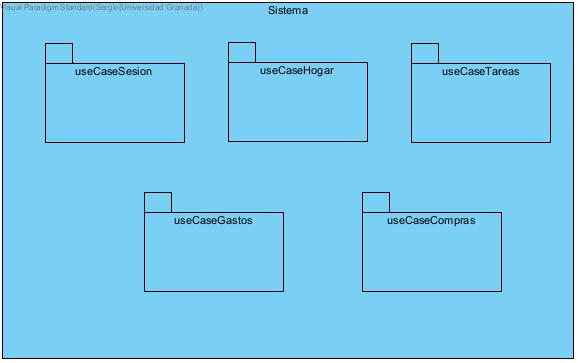
\includegraphics[width=\textwidth]{../capitulos/img/diagrama_paquetes.jpg}
    \caption{Diagrama de paquetes de casos de uso}
    \label{fig:diagrama_paquetes_casos_uso}
\end{figure}


\begin{figure}[htb!]
    \centering
    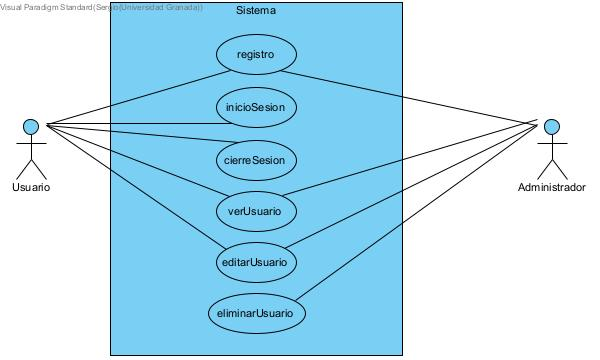
\includegraphics[width=\textwidth]{../capitulos/img/diagrama_sesion.jpg}
    \caption{Diagrama de casos de uso de la gestión de sesión}
    \label{fig:diagrama_sesion_casos_uso}
\end{figure}

\begin{figure}[htb!]
    \centering
    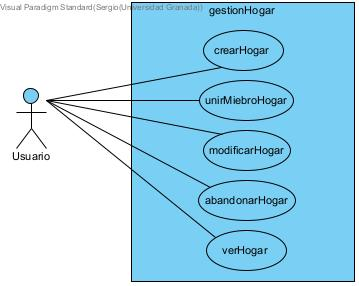
\includegraphics[width=\textwidth]{../capitulos/img/diagrama_hogar.jpg}
    \caption{Diagrama de casos de uso de la gestion de hogar}
    \label{fig:diagrama_hogar_casos_uso}
\end{figure}

\begin{figure}[htb!]
    \centering
    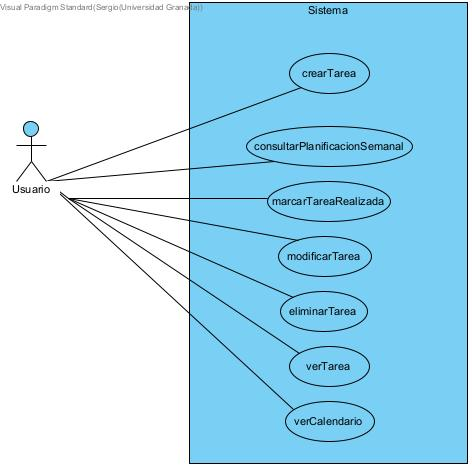
\includegraphics[width=\textwidth]{../capitulos/img/diagrama_tareas.jpg}
    \caption{Diagrama de casos de uso de la gestion de tareas}
    \label{fig:diagrama_tareas_casos_uso}
\end{figure}


\begin{figure}[htb!]
    \centering
    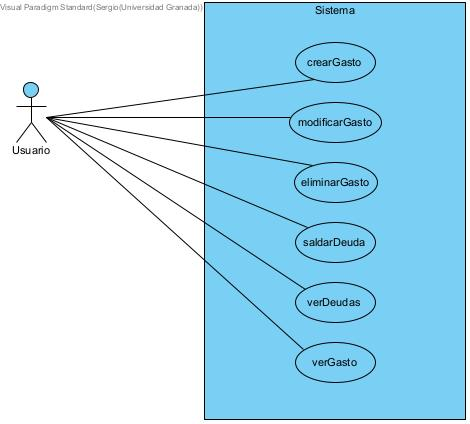
\includegraphics[width=\textwidth]{../capitulos/img/diagrama_gastos.jpg}
    \caption{Diagrama de casos de uso de la gestion de gastos}
    \label{fig:diagrama_gastos_casos_uso}
\end{figure}


\begin{figure}[htb!]
    \centering
    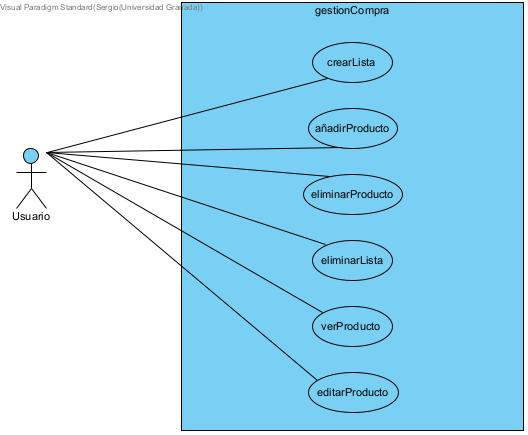
\includegraphics[width=\textwidth]{../capitulos/img/diagrama_compra.jpg}
    \caption{Diagrama de casos de uso de la gestion de compra}
    \label{fig:diagrama_compra_casos_uso}
\end{figure}

\clearpage

\subsection{Descripción de los casos de uso}

En esta sección se describen los casos de uso de la aplicación, indicando los actores involucrados, 
la descripción y los pasos a seguir para llevar a cabo la funcionalidad.



\begin{table}[H]
	\centering
	\begin{tabular}{| m{0.2\textwidth} | m{0.2\textwidth} | m{0.2\textwidth} | m{0.2\textwidth} |}
		\hline
		\rowcolor[HTML]{C0C0C0} Caso de Uso & \multicolumn{2}{|m{0.43\textwidth}|}{registro} &  CU1\\ 
		\hline
		Actores & \multicolumn{3}{l|}{Usuario, Administrador} \\ 
		\hline
		Tipo & \multicolumn{3}{l|}{Obligatorio} \\ 
		\hline
		Referencias & \multicolumn{3}{l|}{\hyperref[req:RF01]{RF\_01}} \\ 
		\hline
		Precondición & \multicolumn{3}{l|}{El usuario no debe estar registrado en el sistema.} \\ 
		\hline
        Postcondición & \multicolumn{3}{l|}{El usuario queda registrado en el sistema.} \\ 
		\hline
		Autor & \multicolumn{3}{l|}{Sergio Muñoz} \\ 
		\hline
		Fecha & 28/02/2025 & Versión & 1.0 \\
		\hline
	\end{tabular}
\end{table}

\begin{table}[H]
	\centering
	\begin{tabular}{| m{0.2\textwidth} | m{0.2\textwidth} | m{0.2\textwidth} | m{0.2\textwidth} |}
		\hline
		Propósito & \multicolumn{3}{m{0.67\textwidth}|}{El usuario debe ser capaz de crearse una cuenta en el sistema.}   \\ 
		\hline
		Resumen & \multicolumn{3}{m{0.67\textwidth}|}{El usuario introduce los datos necesarios para crear una cuenta.} \\ 
		\hline
	\end{tabular}
\end{table}

\begin{table}[H]
	\centering
	\begin{tabular}{| m{0.03\textwidth} | m{0.37\textwidth} | m{0.03\textwidth} | m{0.37\textwidth} |}
		\hline
		\multicolumn{4}{|m{0.9\textwidth}|}{Curso normal}     \\ 
		\hline
		1. & Usuario: Introduce su nombre, apellidos, correo electrónico y contraseña. 
        & 2. & El sistema verifica que los campos no estén vacíos y que la información introducida sea válida. \\ 
		\hline
		3. & Usuario: Confirma el registro. & 4. & El sistema verifica que el correo electrónico no esté registrado previamente.   \\ 
		\hline
        5. & Usuario: Recibe un mensaje indicando que debe verificar su correo electrónico. & 6. & El sistema redirige al usuario a la pantalla de inicio de sesión. \\ 
        \hline
		\multicolumn{4}{|m{0.9\textwidth}|}{Cursos alternos}     \\
        \hline 
        2a. & \multicolumn{3}{l|}{Los campos están vacíos o la información no es válida.} \\ 
        \hline
        2b. & \multicolumn{3}{l|}{El correo electrónico ya está registrado.} \\ 
        \hline
        2c. & \multicolumn{3}{l|}{El sistema muestra un mensaje de error.} \\ 
        \hline
	\end{tabular}
	\caption{Caso de uso - Registro}
\end{table}

\begin{table}[H]
    \centering
    \begin{tabular}{| m{0.2\textwidth} | m{0.2\textwidth} | m{0.2\textwidth} | m{0.2\textwidth} |}
        \hline
        \rowcolor[HTML]{C0C0C0} Caso de Uso & \multicolumn{2}{|m{0.43\textwidth}|}{iniciarSesion} &  CU2\\ 
        \hline
        Actores & \multicolumn{3}{l|}{Usuario} \\ 
        \hline
        Tipo & \multicolumn{3}{l|}{Obligatorio} \\ 
        \hline
        Referencias & \multicolumn{3}{l|}{\hyperref[req:RF02]{RF\_02}} \\ 
        \hline
        Precondición & \multicolumn{3}{l|}{El usuario debe estar registrado en el sistema.} \\ 
        \hline
        Postcondición & \multicolumn{3}{l|}{El usuario accede al sistema.} \\ 
        \hline
        Autor & \multicolumn{3}{l|}{Sergio Muñoz} \\ 
        \hline
        Fecha & 28/02/2025 & Versión & 1.0 \\
        \hline
    \end{tabular}
\end{table}

\begin{table}[H]
    \centering
    \begin{tabular}{| m{0.2\textwidth} | m{0.2\textwidth} | m{0.2\textwidth} | m{0.2\textwidth} |}
        \hline
        Propósito & \multicolumn{3}{m{0.67\textwidth}|}{El usuario debe ser capaz de iniciar sesión en el sistema.}   \\ 
        \hline
        Resumen & \multicolumn{3}{m{0.67\textwidth}|}{El usuario introduce su correo electrónico y contraseña para autenticarse.} \\ 
        \hline
    \end{tabular}
\end{table}



\begin{table}[H]
    \centering
    \begin{tabular}{| m{0.03\textwidth} | m{0.37\textwidth} | m{0.03\textwidth} | m{0.37\textwidth} |}
        \hline
        \multicolumn{4}{|m{0.9\textwidth}|}{Curso normal}     \\ 
        \hline
        1. & Usuario: Introduce su correo electrónico y contraseña. 
        & 2. & El sistema verifica que los campos no estén vacíos y que la información introducida sea válida. \\ 
        \hline
        3. & Usuario: Confirma el inicio de sesión. & 4. & El sistema verifica que el correo electrónico y la contraseña sean correctos.   \\ 
        \hline
        5. & Usuario: Accede a la pantalla principal de la aplicación. & 6. & El sistema redirige al usuario a la pantalla principal de la aplicación. \\ 
        \hline
        \multicolumn{4}{|m{0.9\textwidth}|}{Cursos alternos}     \\
        \hline 
        2a. & \multicolumn{3}{l|}{Los campos están vacíos o la información no es válida.} \\ 
        \hline
        2b. & \multicolumn{3}{l|}{El correo electrónico o la contraseña son incorrectos.} \\ 
        \hline
        2c. & \multicolumn{3}{l|}{El sistema muestra un mensaje de error.} \\ 
        \hline
    \end{tabular}
    \caption{Caso de uso - Iniciar Sesión}
\end{table}

\newpage

\begin{table}[H]
    \centering
    \begin{tabular}{| m{0.2\textwidth} | m{0.2\textwidth} | m{0.2\textwidth} | m{0.2\textwidth} |}
        \hline
        \rowcolor[HTML]{C0C0C0} Caso de Uso & \multicolumn{2}{|m{0.43\textwidth}|}{cerrarSesion} &  CU3\\ 
        \hline
        Actores & \multicolumn{3}{l|}{Usuario} \\ 
        \hline
        Tipo & \multicolumn{3}{l|}{Obligatorio} \\ 
        \hline
        Referencias & \multicolumn{3}{l|}{\hyperref[req:RF04]{RF\_04}} \\ 
        \hline
        Precondición & \multicolumn{3}{l|}{El usuario debe estar autenticado en el sistema.} \\ 
        \hline
        Postcondición & \multicolumn{3}{l|}{El usuario cierra su sesión en el sistema.} \\ 
        \hline
        Autor & \multicolumn{3}{l|}{Sergio Muñoz} \\ 
        \hline
        Fecha & 28/02/2025 & Versión & 1.0 \\ 
        \hline
    \end{tabular}
\end{table}

\begin{table}[H]
    \centering
    \begin{tabular}{| m{0.2\textwidth} | m{0.2\textwidth} | m{0.2\textwidth} | m{0.2\textwidth} |}
        \hline
        Propósito & \multicolumn{3}{m{0.67\textwidth}|}{El usuario debe ser capaz de cerrar su sesión en el sistema.} \\ 
        \hline
        Resumen & \multicolumn{3}{m{0.67\textwidth}|}{El usuario cierra su sesión para finalizar su uso del sistema.} \\ 
        \hline
    \end{tabular}
\end{table}

\begin{table}[H]
    \centering
    \begin{tabular}{| m{0.03\textwidth} | m{0.37\textwidth} | m{0.03\textwidth} | m{0.37\textwidth} |}
        \hline
        \multicolumn{4}{|m{0.9\textwidth}|}{Curso normal} \\ 
        \hline
        1. & Usuario: Pulsa el botón de cerrar sesión. 
        & 2. & El sistema muestra un mensaje de confirmación. \\ 
        \hline
        3. & Usuario: Confirma que desea cerrar sesión. 
        & 4. & El sistema cierra la sesión del usuario y redirige a la pantalla de inicio de sesión. \\ 
        \hline
    \end{tabular}
    \caption{Caso de uso - Cerrar Sesión}
\end{table}


La explicación de los casos de uso restantes se encuentra en el Apéndice \ref{anexo:casos_de_uso}.
\clearpage 



%
\chapter{Diseño}

\section{Diseño de la arquitectura}
\label{sec:arquitectura}
La arquitectura de este sistema se basa en un modelo \textbf{cliente-base de datos}, donde el usuario interactúa únicamente con 
la interfaz gráfica de la aplicación (cliente), la cual se comunica con la base de datos \textit{Firebase Firestore} para obtener y almacenar la información. 
La interfaz gráfica se interactua directamente con la base de datos, sin necesidad de un servidor intermedio. Esta estructura simplifica el
desarrolo, al delegar en Firebase la gestión de la base de datos y la sincronización en tiempo real.

\subsection{Componentes Principales}

\begin{itemize}
    \item \textbf{Interfaz gráfica:} La interfaz gráfica es la parte de la aplicación con la que el usuario interactúa. 
    En este caso, la interfaz gráfica se ha diseñado para ser intuitiva y fácil de usar, con el objetivo de que el usuario pueda 
    realizar las tareas de forma rápida y sencilla.
    \item \textbf{Base de datos:} La base de datos es el componente encargado de almacenar y gestionar la información de la aplicación. 
    En este caso, se ha utilizado Firebase Firestore como base de datos, ya que permite almacenar y sincronizar los datos en tiempo real, 
    lo que facilita la gestión de la información.
\end{itemize}

\subsection{Flujo de interacción}

\begin{enumerate}
    \item El usuario accede a la aplicación y realiza una acción.
    \item La interfaz gráfica procesa la acción y envía la solicitud a la base de datos a través de las funciones de Firebase.
    \item La base de datos recibe la solicitud, la procesa y devuelve la información necesaria
    \item La interfaz gráfica recibe la información y la muestra al usuario.
\end{enumerate}


\section{Diseño de la interfaz gráfica}
\label{sec:interfaz}
El objetivo principal es conseguir la usabilidad de la aplicación, ya que aunque la aplicaciónn esté dirigida a un público joven, 
es importante que sea fácil de usar para cualquier usuario. Para ello, se va a diseñar una interfaz gráfica con un diseño sencillo 
teniendo en cuenta los siguientes críterios para que una aplicación sea usable:

\begin{itemize}
    \item \textbf{Simplicidad:} El diseño debe ser sencillo , evitando elementos innecesarios que puedan confundir al usuario.
    \item \textbf{Tamaño de los elementos:} Los elementos de la interfaz gráfica deben tener un tamaño adecuado para que el usuario pueda interactuar con ellos de forma cómoda.
    \item \textbf{Contraste:} Los colores y la tipografía deben tener un contraste adecuado para que el usuario pueda leer la información de forma clara.
    \item \textbf{Facilidad de navegación:} La interfaz gráfica debe ser fácil de navegar, permitiendo al usuario moverse de una pantalla a otra de forma rápida y sencilla.
\end{itemize}
    
\subsection{Interfaces de gráficas del Grupo 1: \textit{Gestión de sesión}}

En esta sección podemos ver todos los diseños de las interfaces gráficas del Grupo 1: \textit{Gestión de sesión}.

\begin{figure}[ht]
    \centering
    \begin{minipage}{0.45\textwidth}
        \centering
        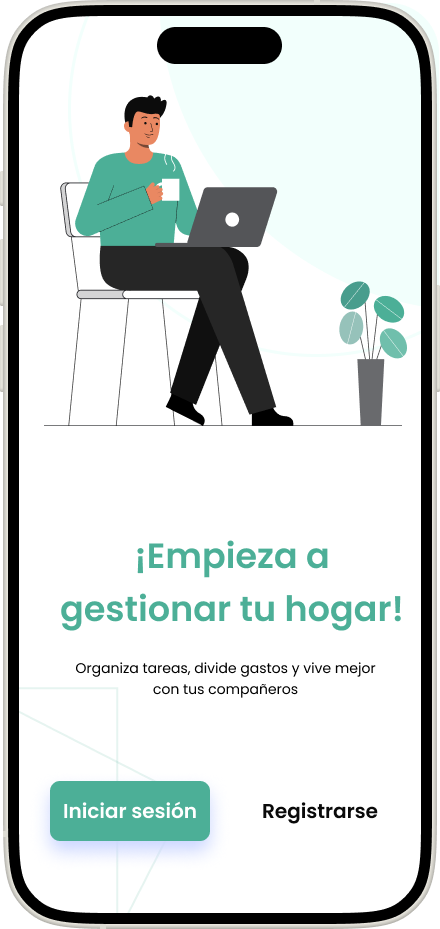
\includegraphics[width=\textwidth]{../capitulos/img/welcome_screen.png}
        \caption{Diseño de la pantalla de bienvenida.}
        \label{welcome}
    \end{minipage}
    \hfill
    \begin{minipage}{0.45\textwidth}
        \centering
        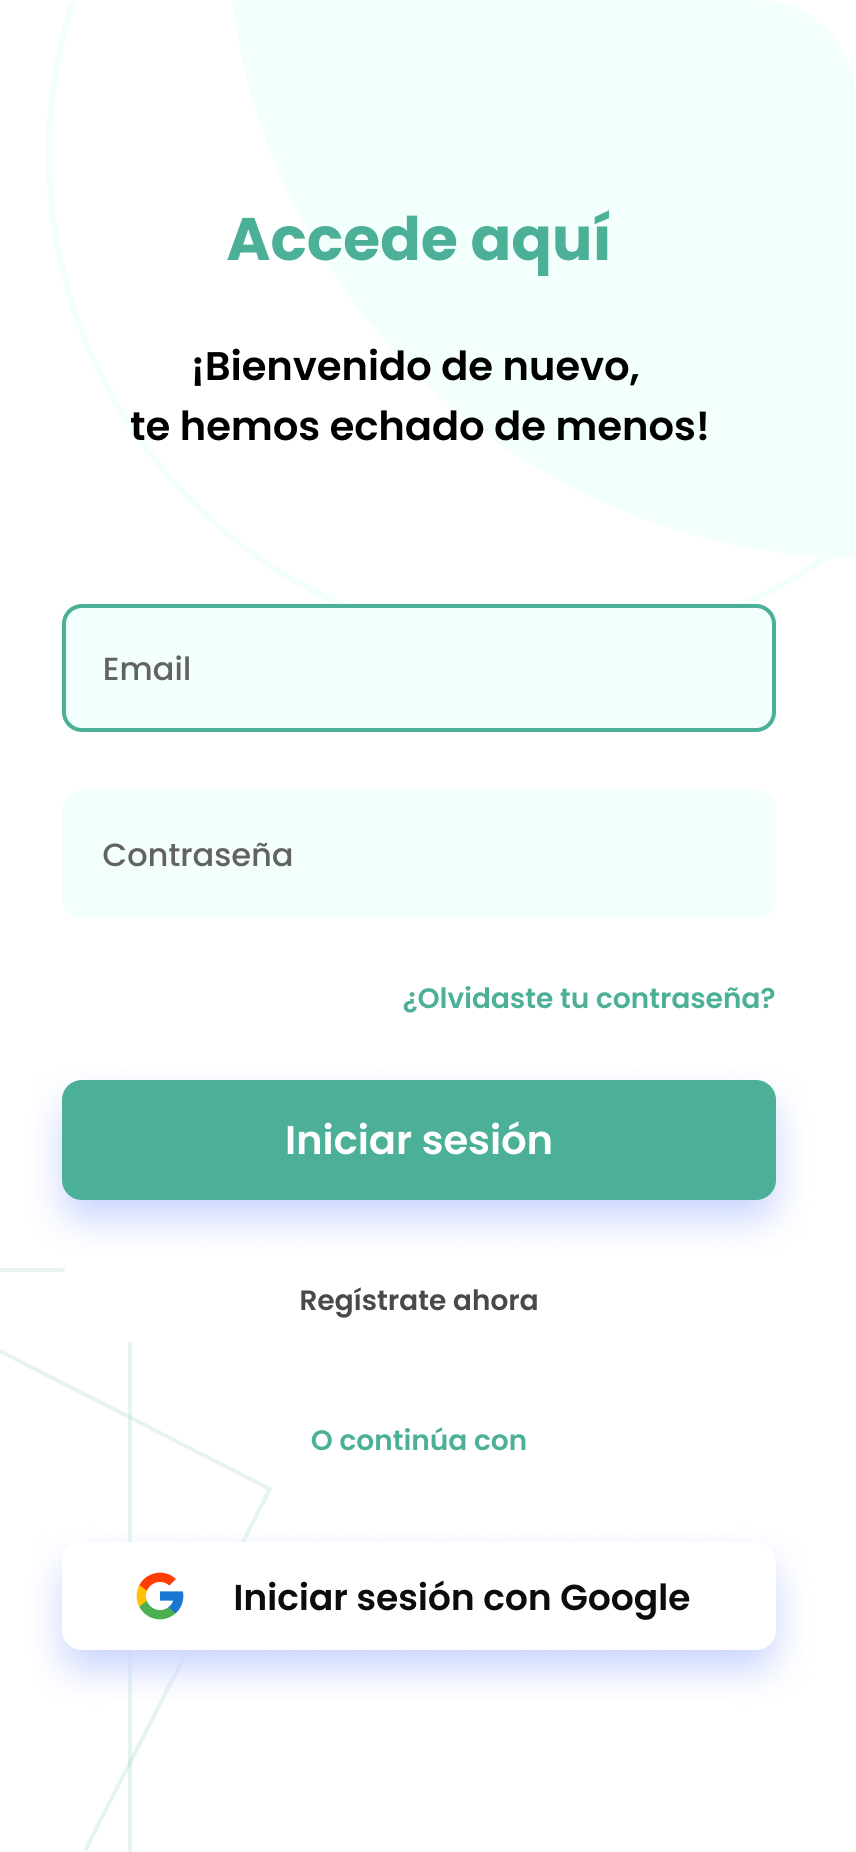
\includegraphics[width=\textwidth]{../capitulos/img/login_screen.png}
        \caption{Diseño de la pantalla de inicio de sesión.}
        \label{login}
    \end{minipage}
\end{figure}


\begin{figure}[ht]
    \centering
    \begin{minipage}{0.45\textwidth}
        \centering
        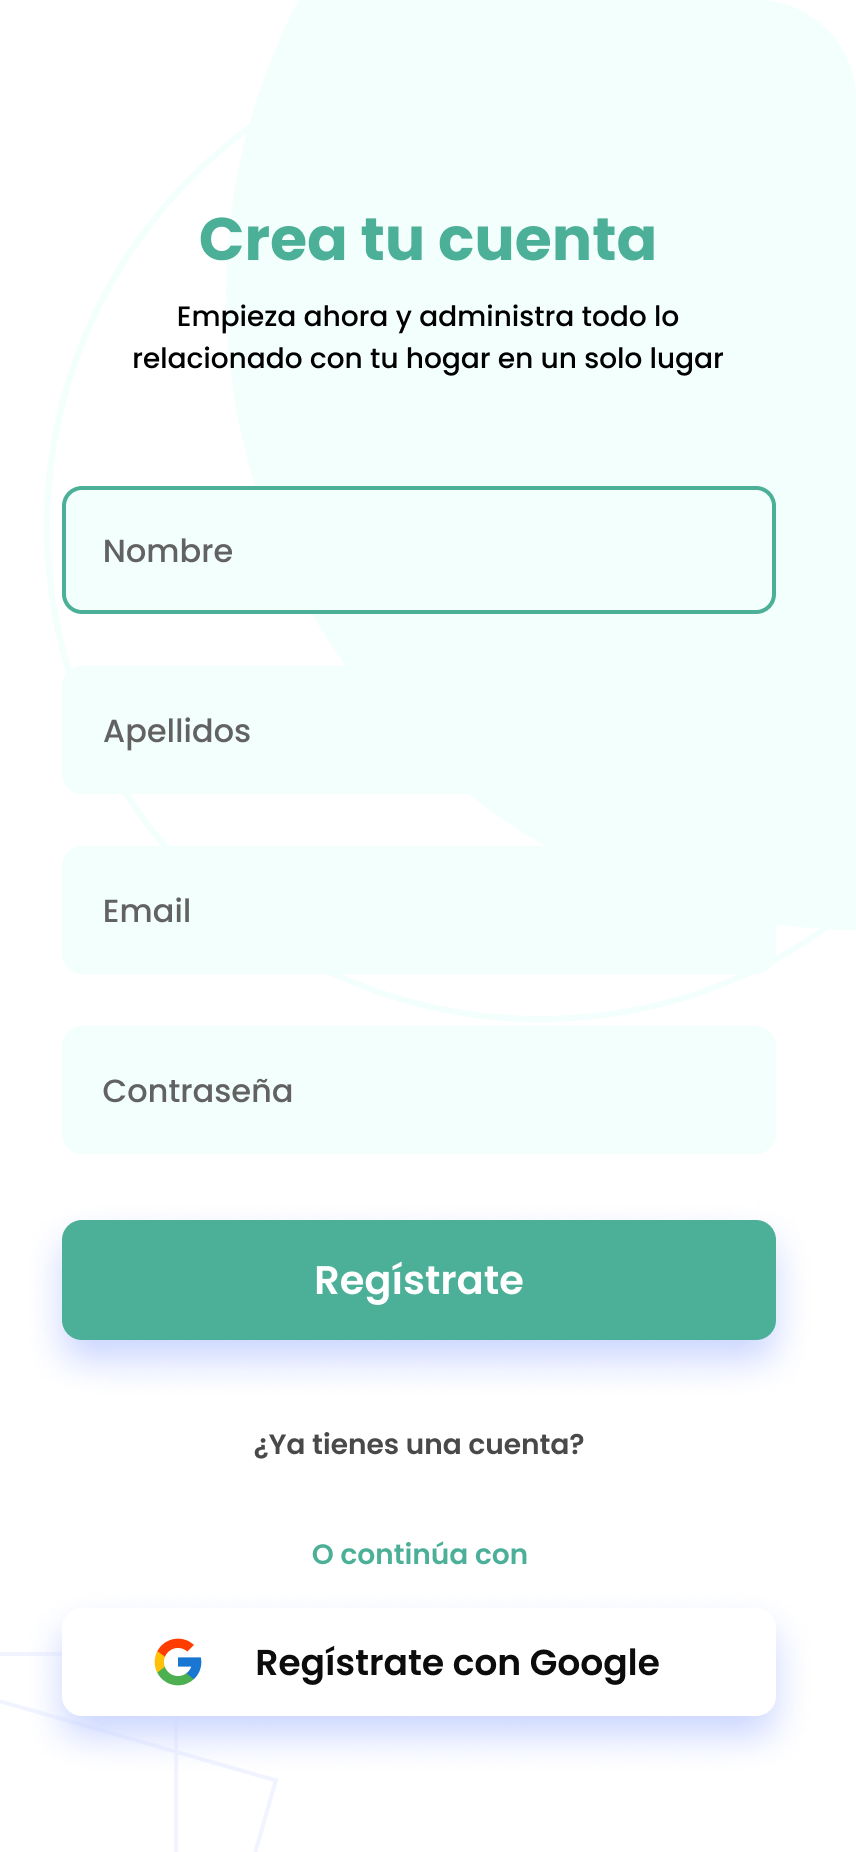
\includegraphics[width=\textwidth]{../capitulos/img/registro_screen.png}
        \caption{Diseño de la pantalla de registro.}
        \label{registro_app}
    \end{minipage}
    \hfill
    \begin{minipage}{0.45\textwidth}
        \centering
        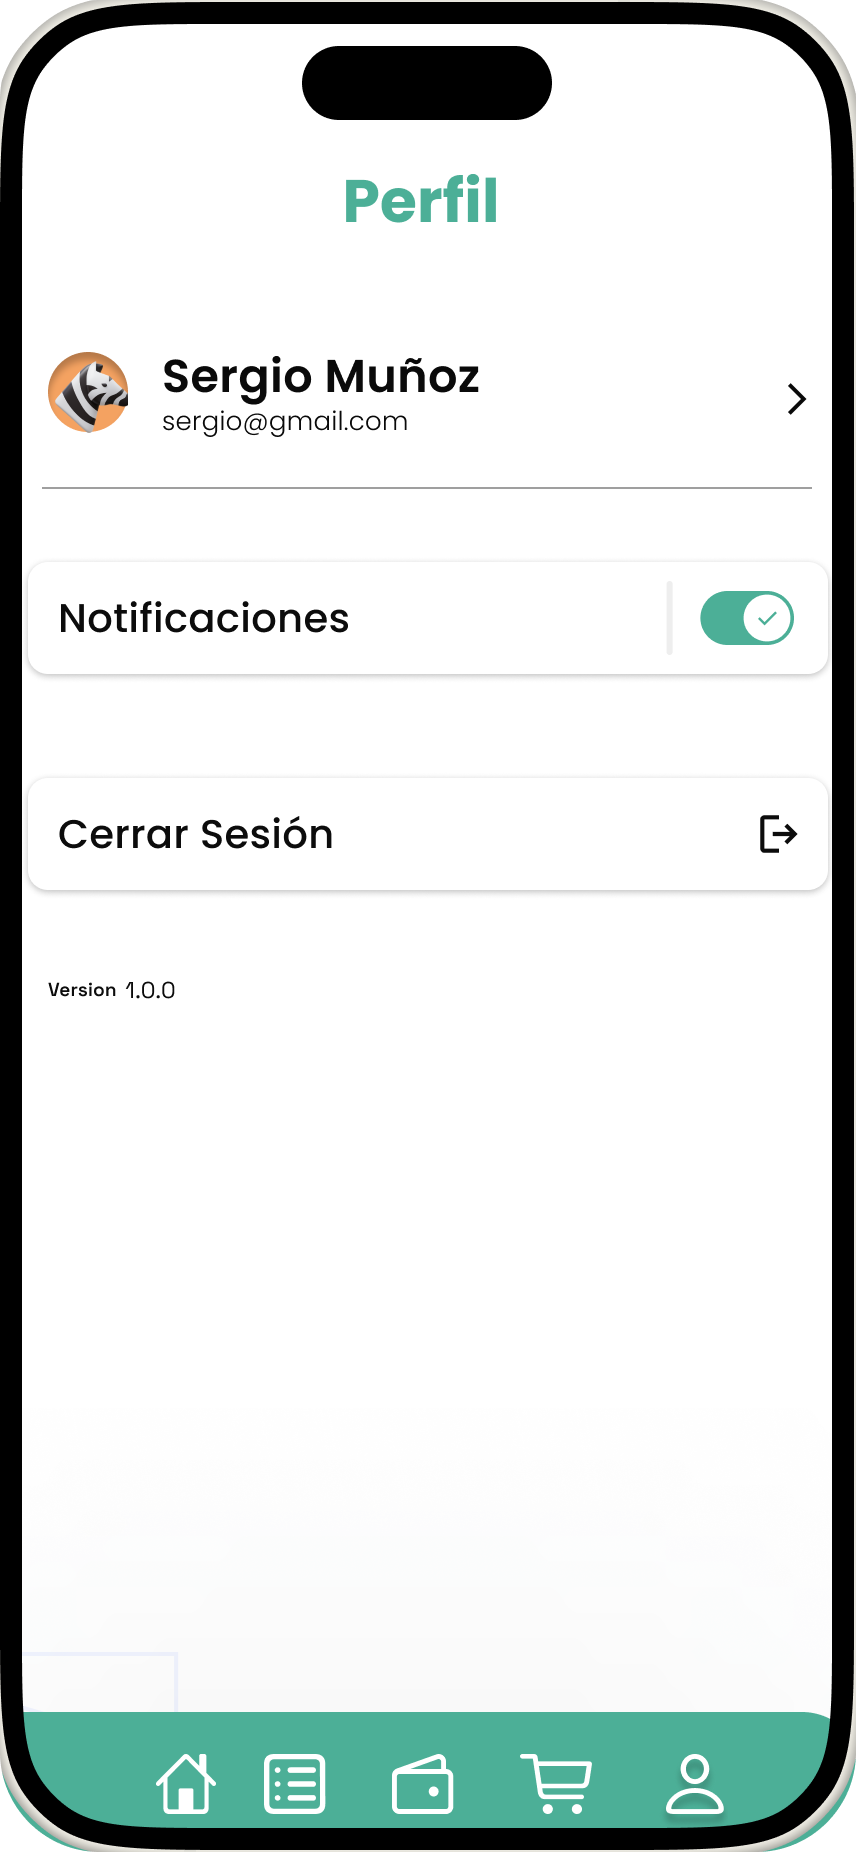
\includegraphics[width=\textwidth]{../capitulos/img/profile_screen.png}
        \caption{Diseño de la pantalla de cierre de sesión y datos de usuario.}
        \label{cierre}
    \end{minipage}
\end{figure}

\begin{figure}[ht]
    \centering
    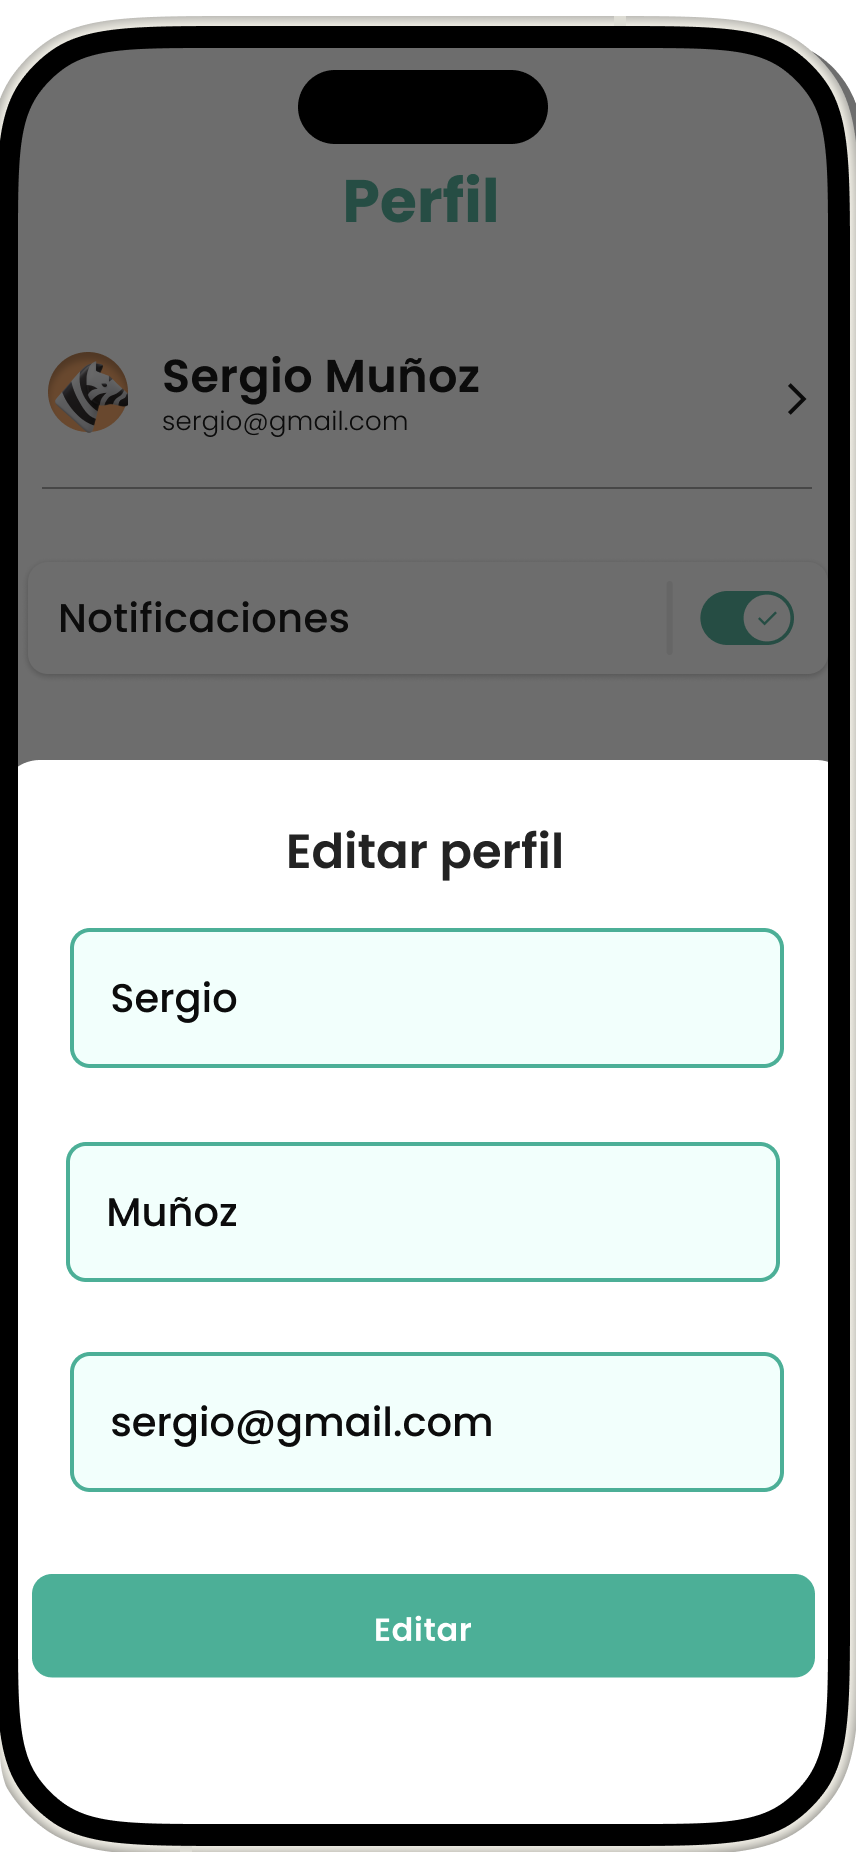
\includegraphics[width=0.45\textwidth]{../capitulos/img/edit_profile_screen.png}
    \caption{Diseño de la pantalla de editar perfil.}
    \label{edit_profile}
\end{figure}

\clearpage

\subsection{Interfaces de gráficas del Grupo 2: \textit{Gestión del hogar}}

\begin{figure}[ht]
    \centering
    \begin{minipage}{0.45\textwidth}
        \centering
        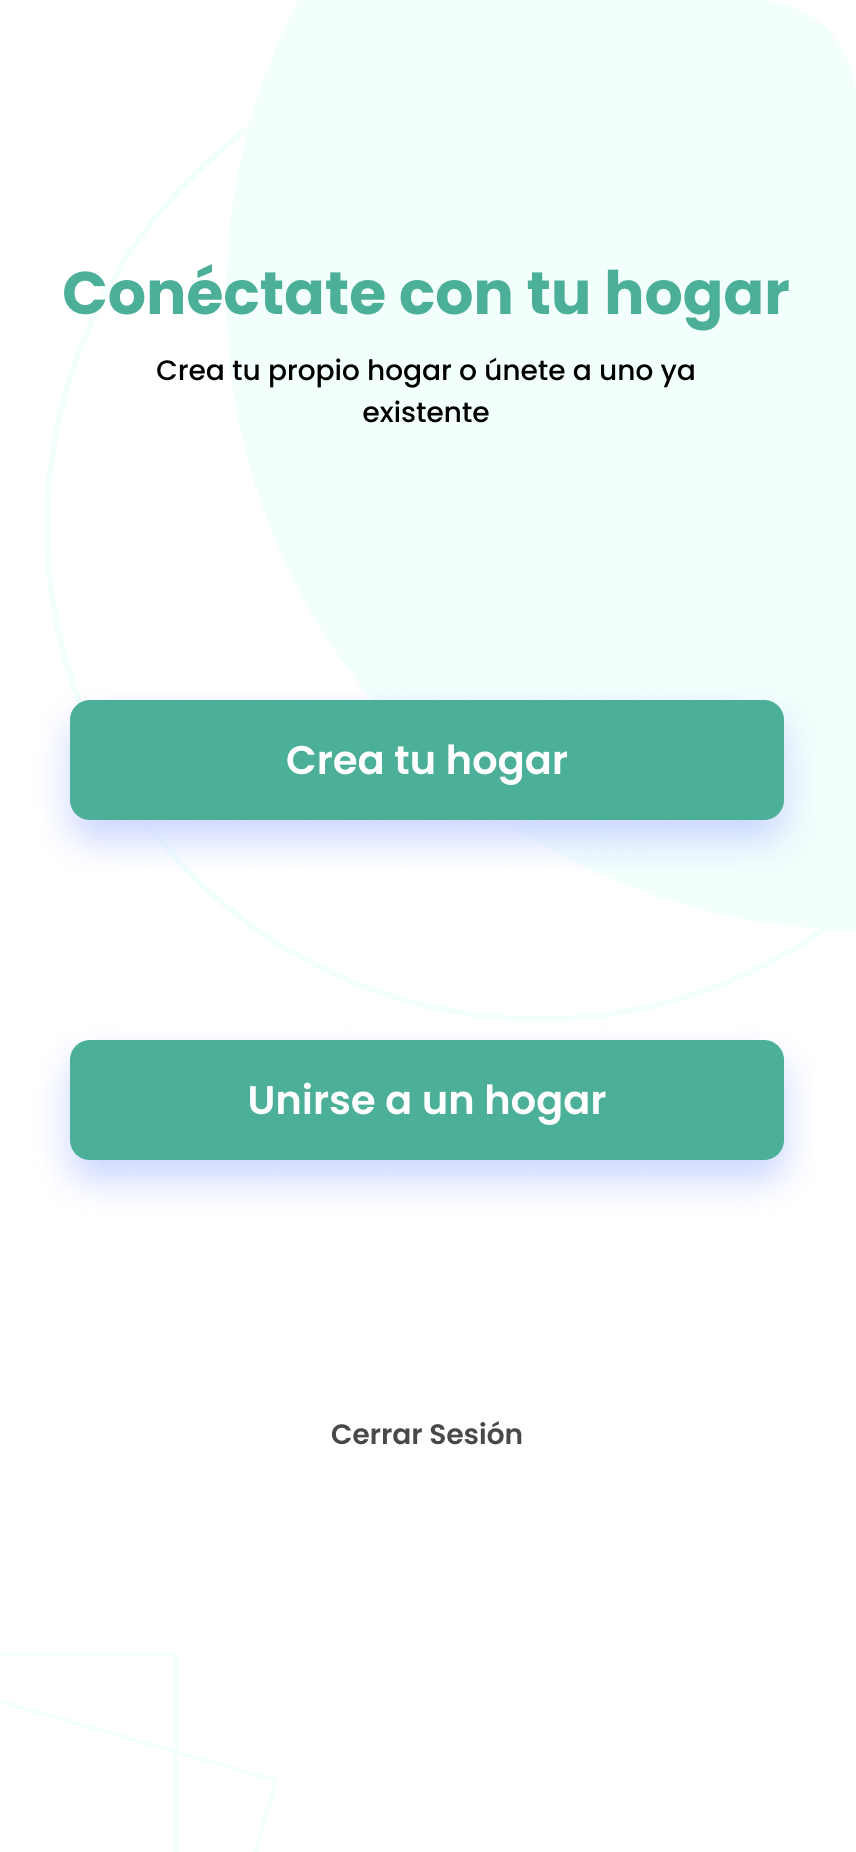
\includegraphics[width=\textwidth]{../capitulos/img/conect_screen.png}
        \caption{Diseño de la pantalla para unirte a un hogar o crear uno nuevo.}
        \label{conect}
    \end{minipage}
    \hfill
    \begin{minipage}{0.45\textwidth}
        \centering
        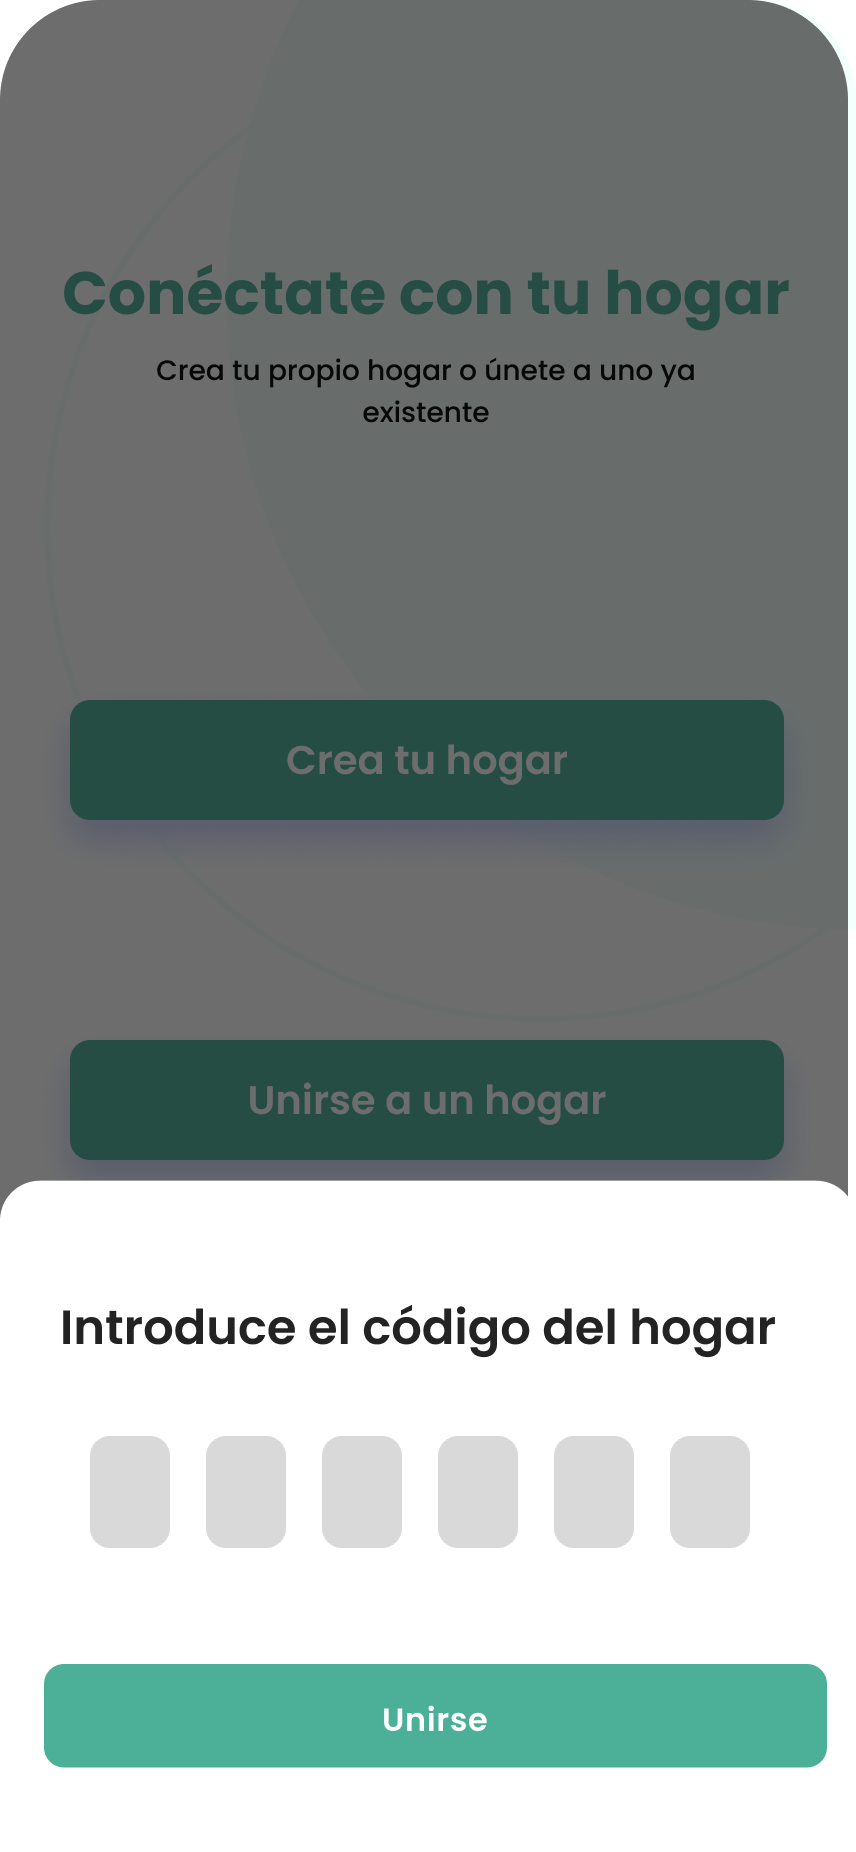
\includegraphics[width=\textwidth]{../capitulos/img/join_screen.png}
        \caption{Diseño de la pantalla para unirte a un hogar.}
        \label{join}
    \end{minipage}
\end{figure}

\begin{figure}[ht]
    \centering
    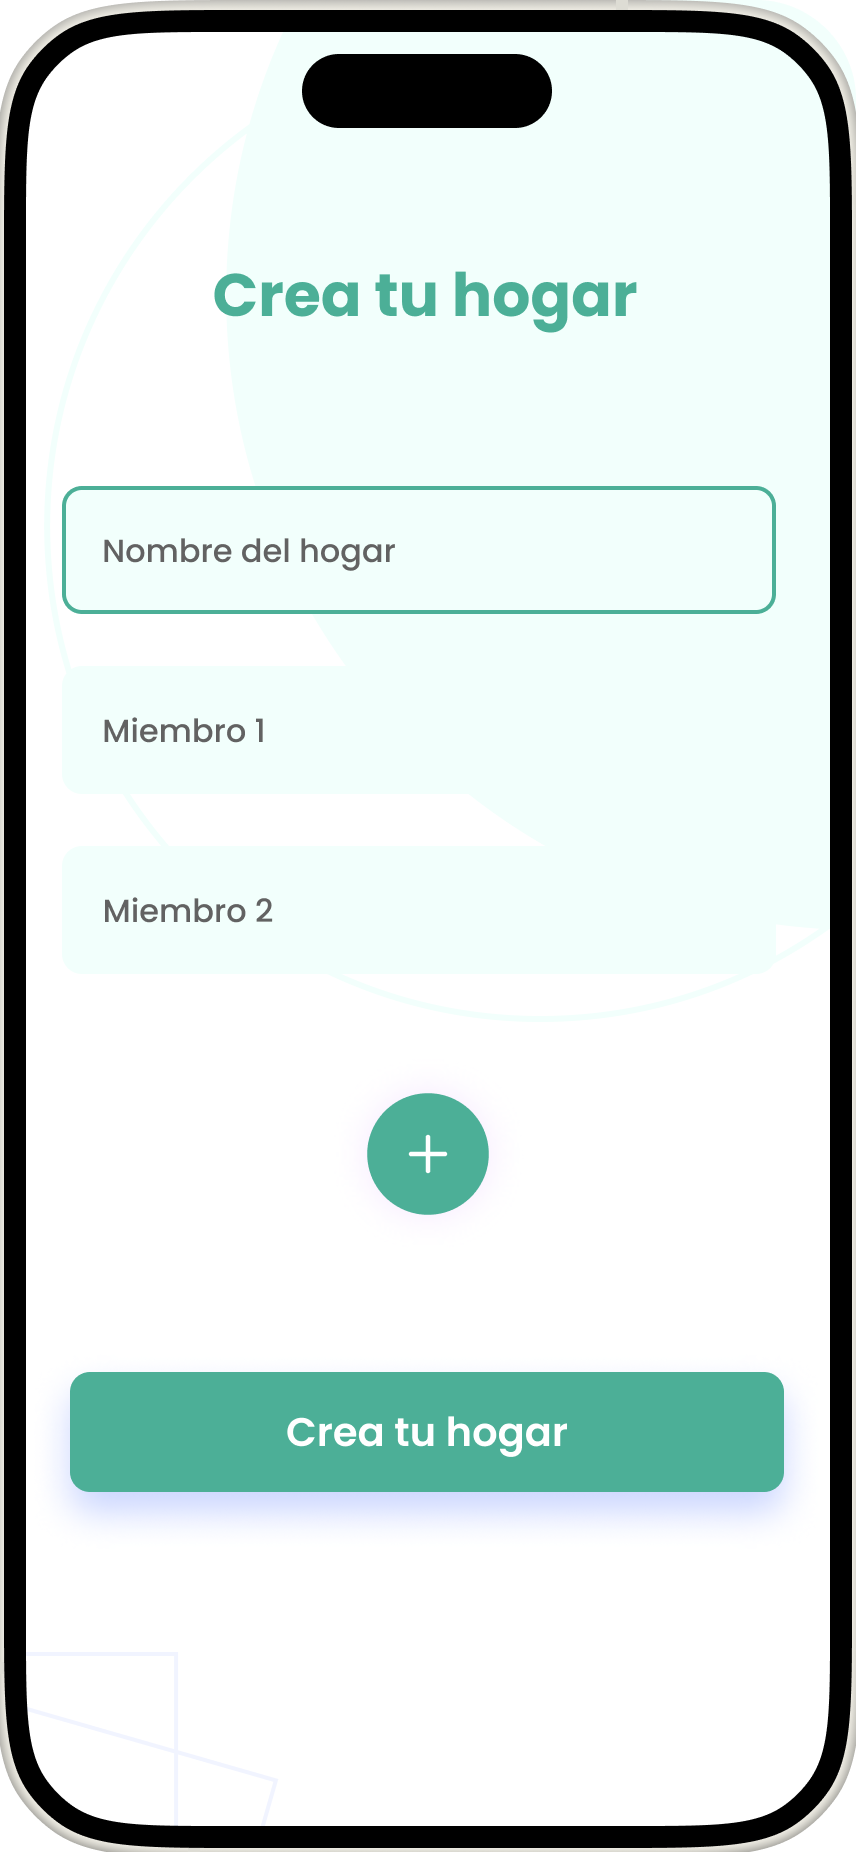
\includegraphics[width=0.45\textwidth]{../capitulos/img/new_home_screen.png}
    \caption{Diseño de la pantalla para crear un nuevo hogar.}
    \label{create_home}
\end{figure}



\clearpage

\subsection{Interfaces de gráficas del Grupo 3: \textit{Gestión de tareas}}

\begin{figure}[ht]
    \centering
    \begin{minipage}{0.45\textwidth}
        \centering
        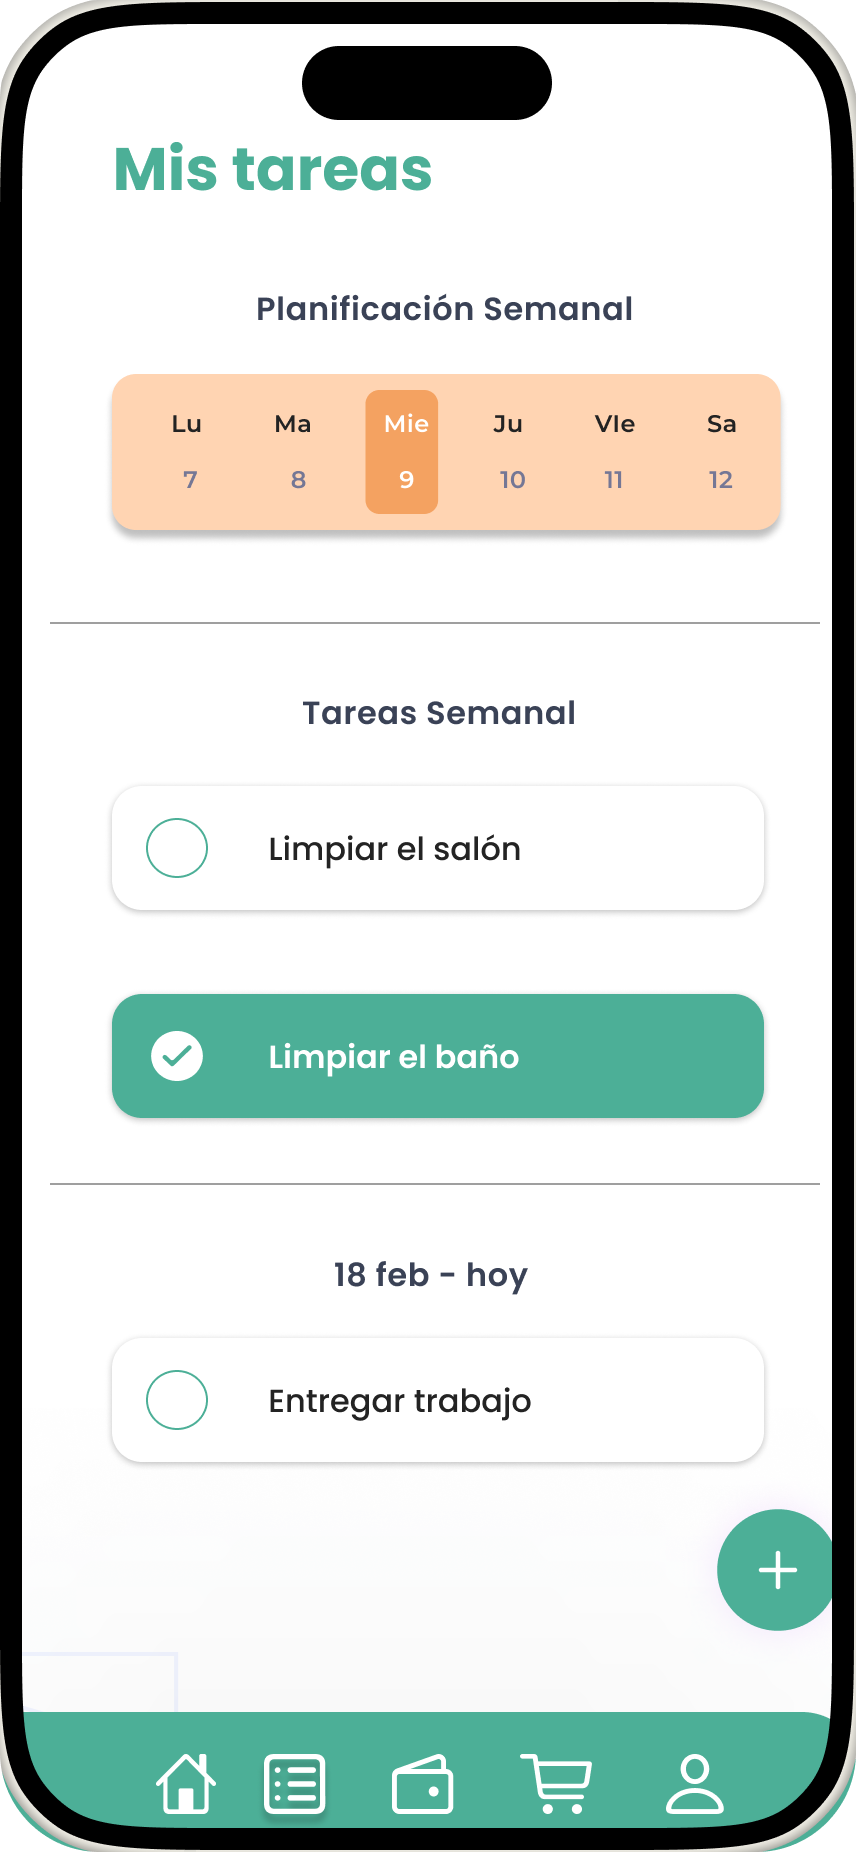
\includegraphics[width=\textwidth]{../capitulos/img/task_screen.png}
        \caption{Diseño de la pantalla principal de tareas.}
        \label{taks}
    \end{minipage}
    \hfill
    \begin{minipage}{0.45\textwidth}
        \centering
        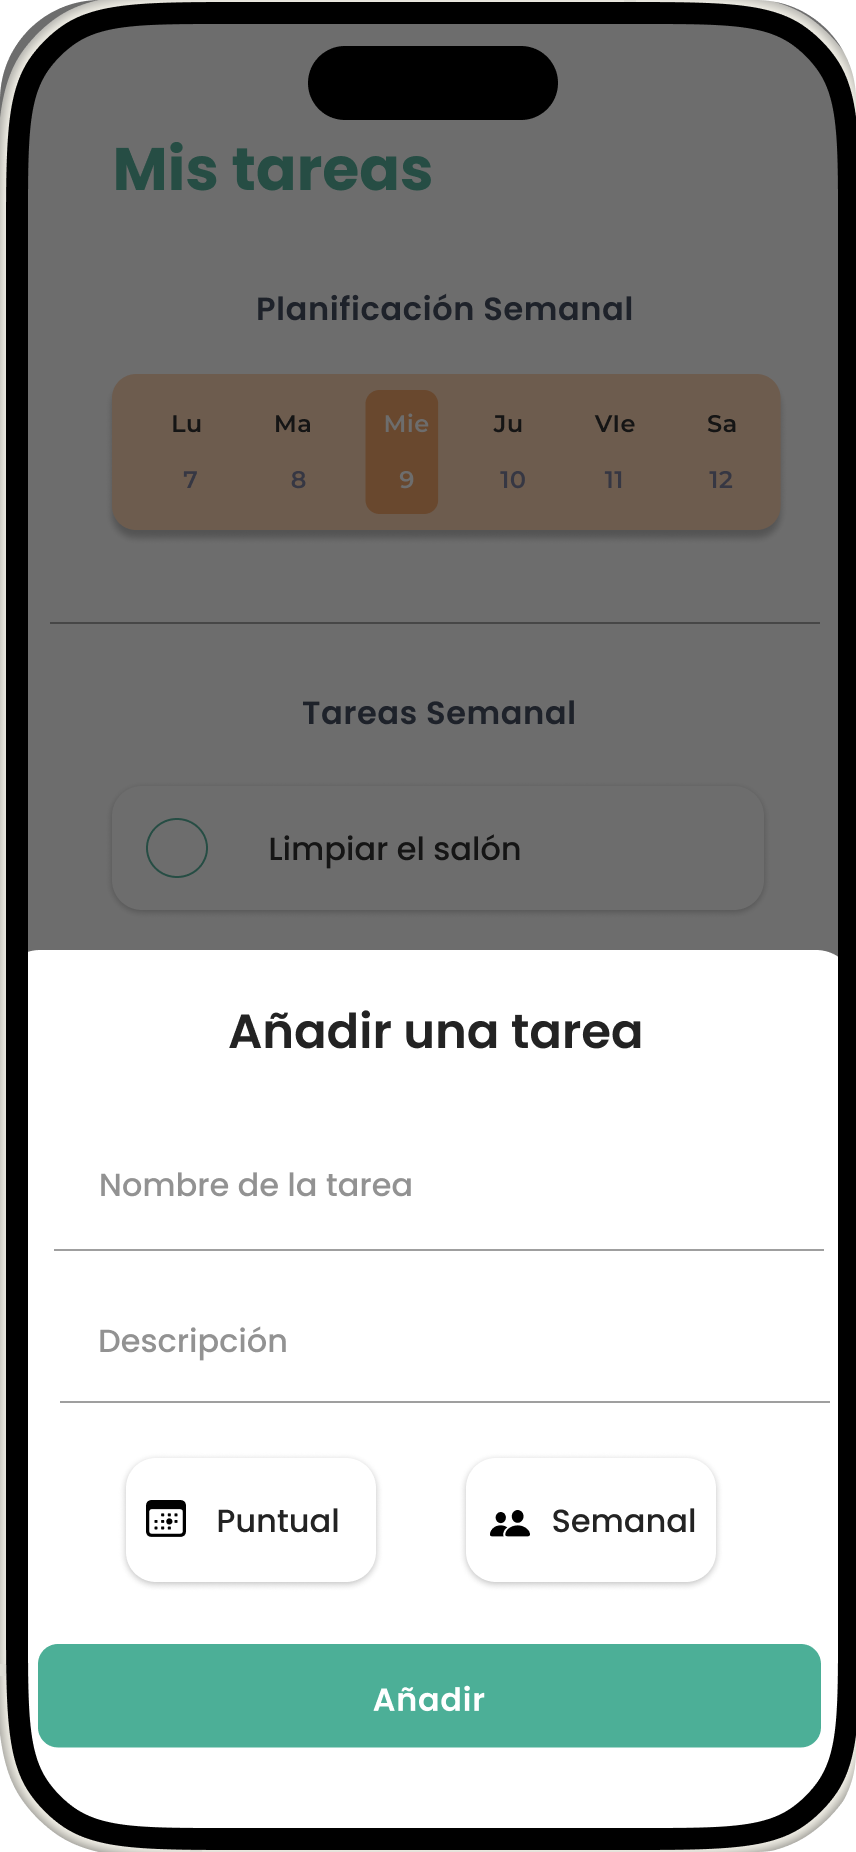
\includegraphics[width=\textwidth]{../capitulos/img/add_tasks_screen.png}
        \caption{Diseño de la pantalla para añadir una tarea.}
        \label{add_task}
    \end{minipage}
\end{figure}

\begin{figure}[ht]
    \centering
    \begin{minipage}{0.45\textwidth}
        \centering
        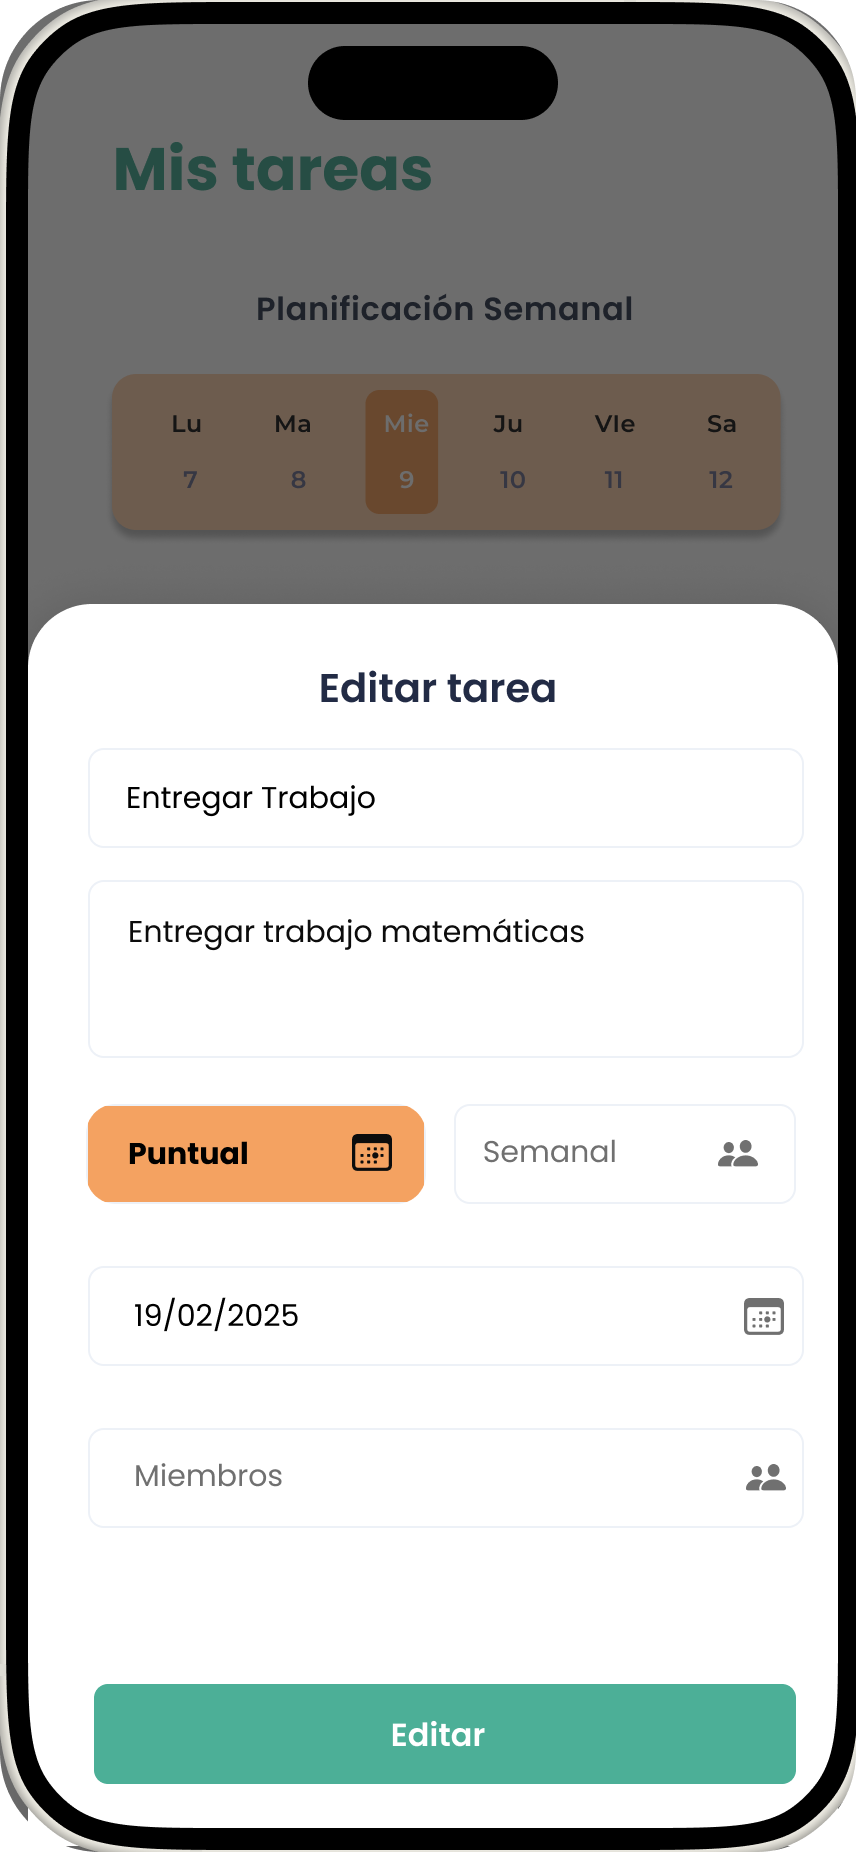
\includegraphics[width=\textwidth]{../capitulos/img/edit_task.png}
        \caption{Diseño de la pantalla para editar una tarea.}
        \label{edit_task}
    \end{minipage}
    \hfill
    \begin{minipage}{0.45\textwidth}
        \centering
        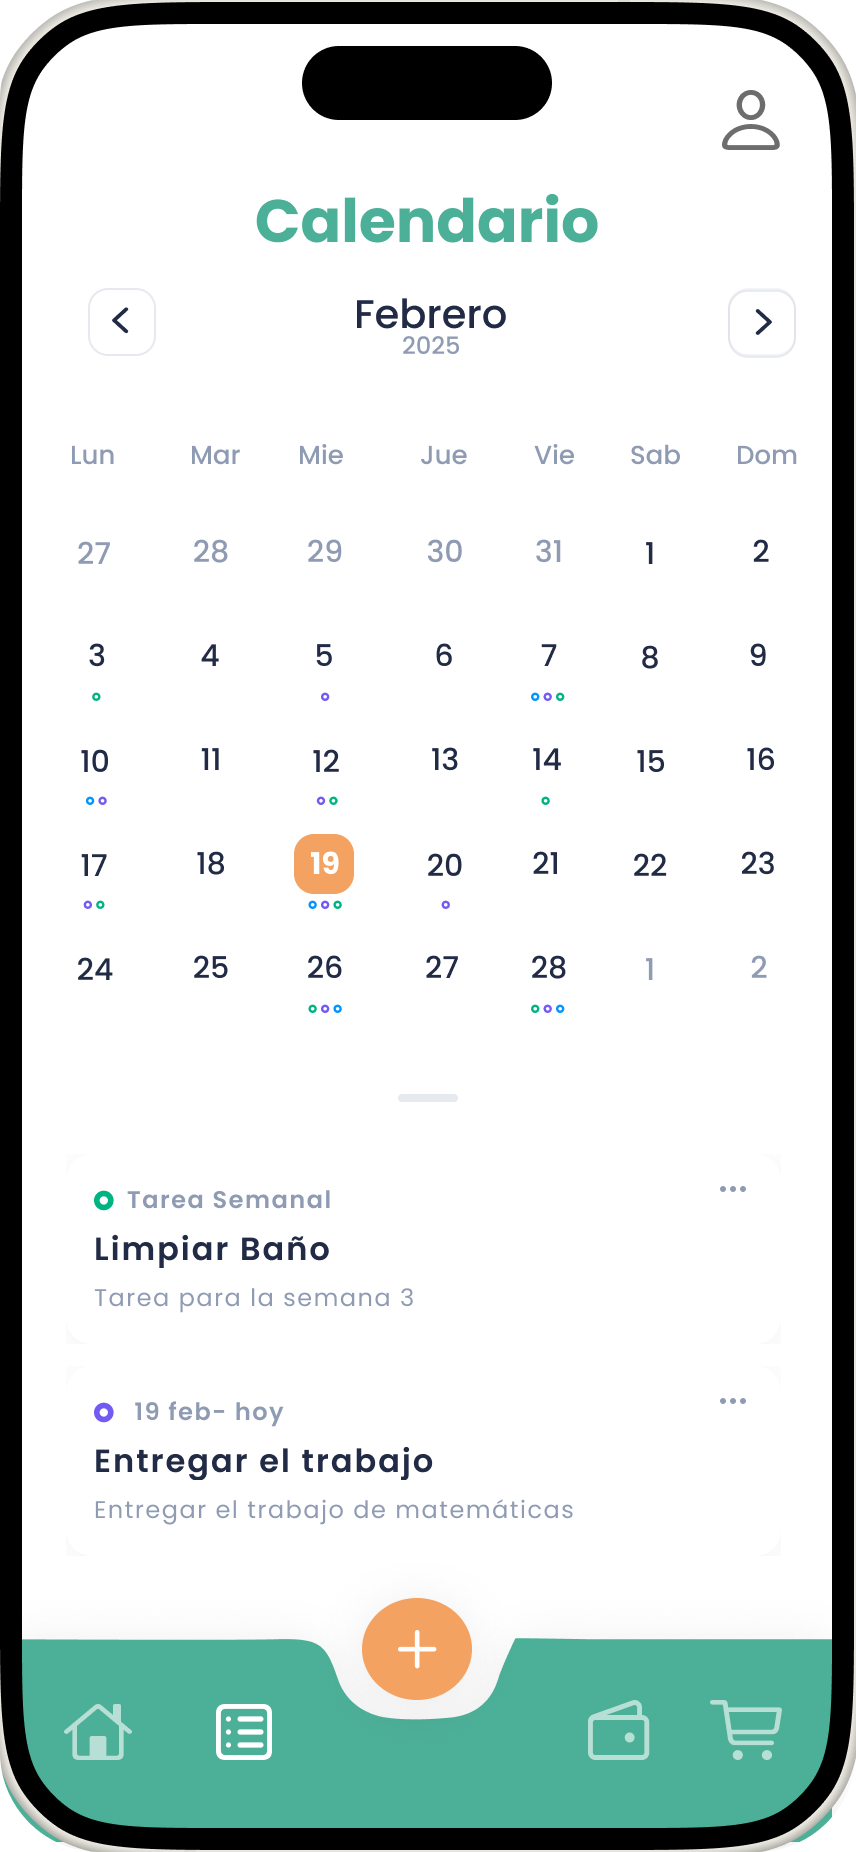
\includegraphics[width=\textwidth]{../capitulos/img/calendar_screen.png}
        \caption{Diseño de la pantalla del calendario.}
        \label{calendar}
    \end{minipage}
\end{figure}


\clearpage

\subsection{Interfaces de gráficas del Grupo 4: \textit{Gestión de gastos}}

\begin{figure}[ht]
    \centering
    \begin{minipage}{0.45\textwidth}
        \centering
        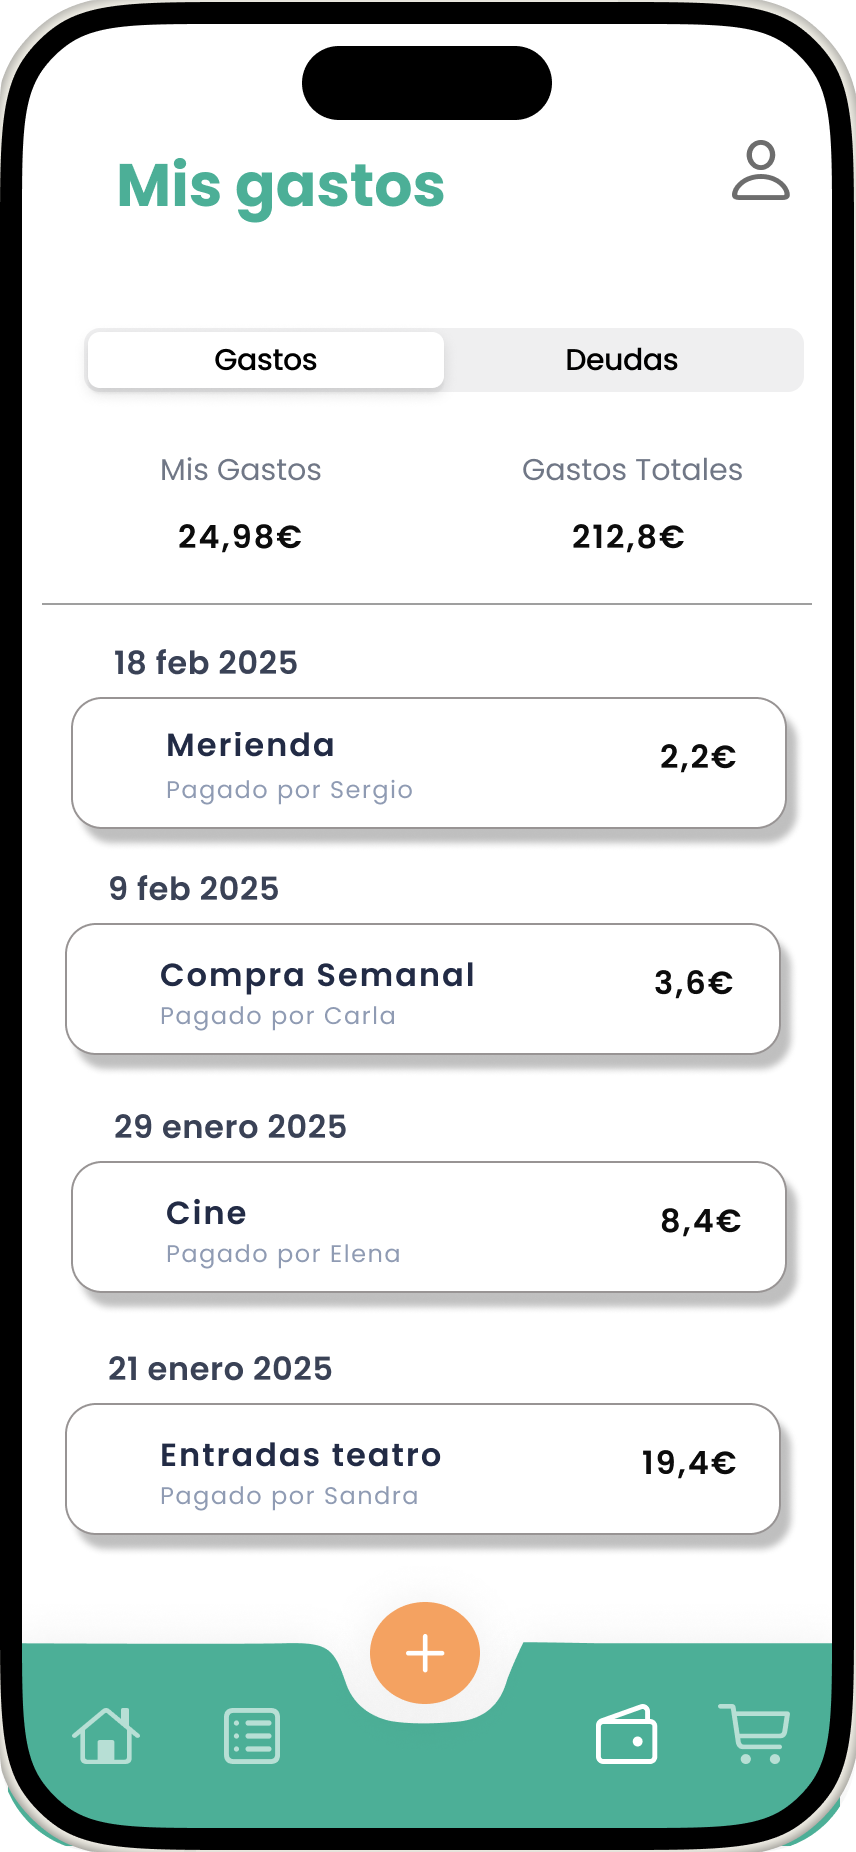
\includegraphics[width=\textwidth]{../capitulos/img/bills_screen.png}
        \caption{Diseño de la pantalla principal de gastos.}
        \label{expenses}
    \end{minipage}
    \hfill
    \begin{minipage}{0.45\textwidth}
        \centering
        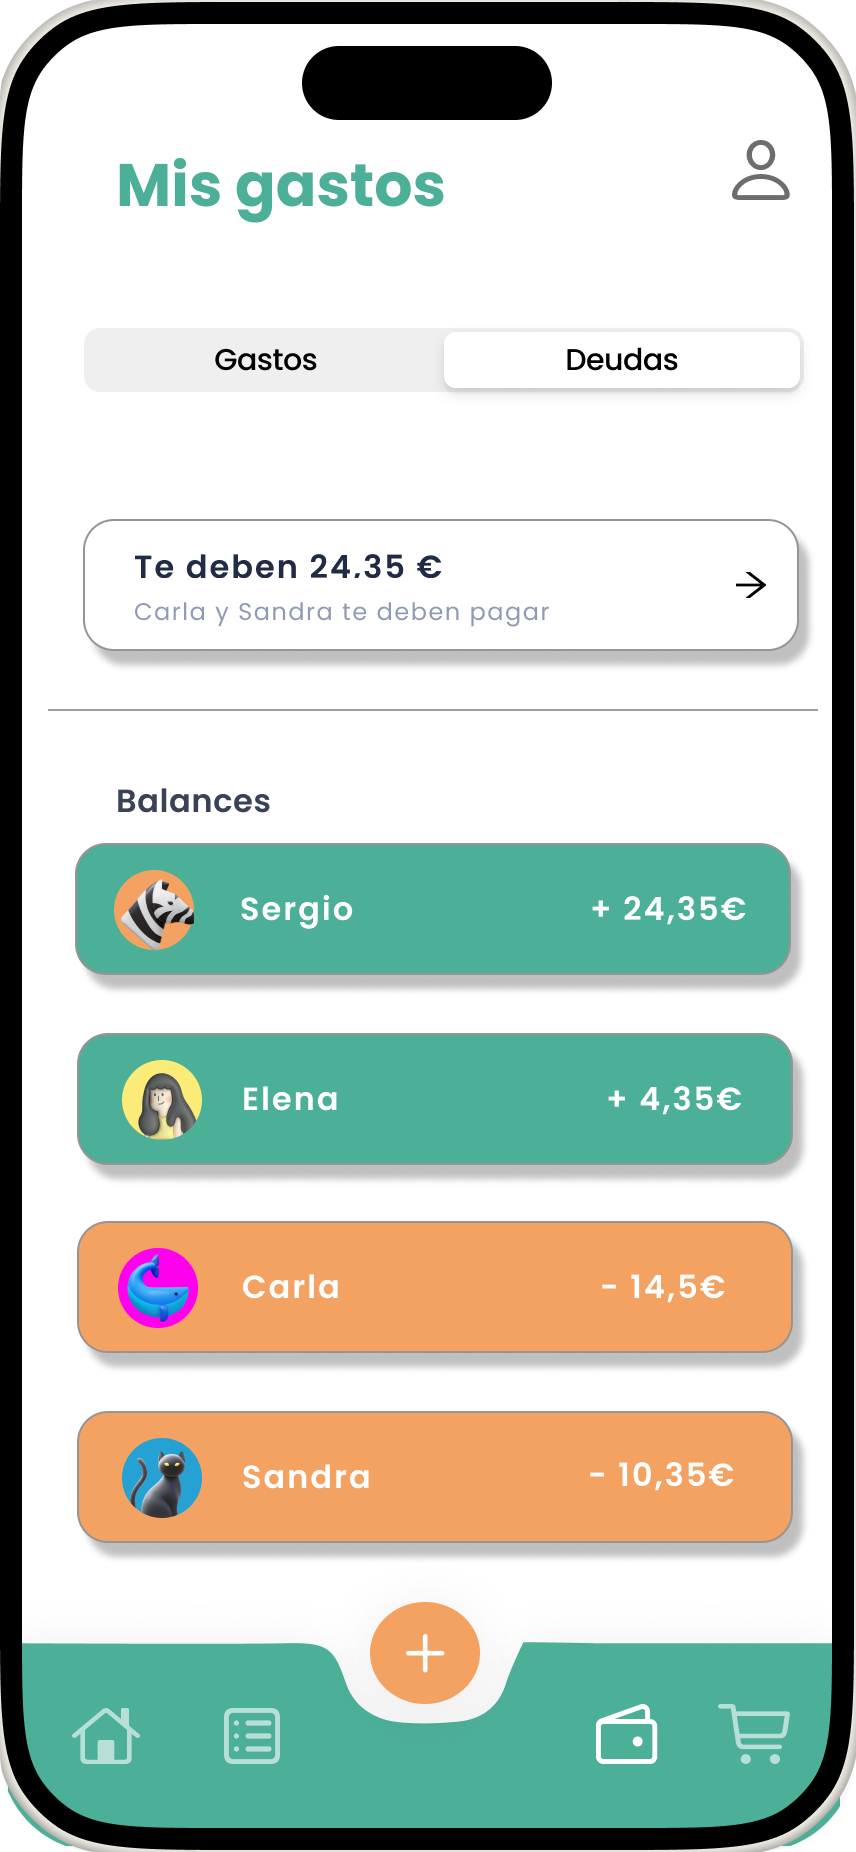
\includegraphics[width=\textwidth]{../capitulos/img/debs_screen.png}
        \caption{Diseño de la pantalla de deudas.}
        \label{debts}
    \end{minipage}
\end{figure}

\begin{figure}[ht]
    \centering
    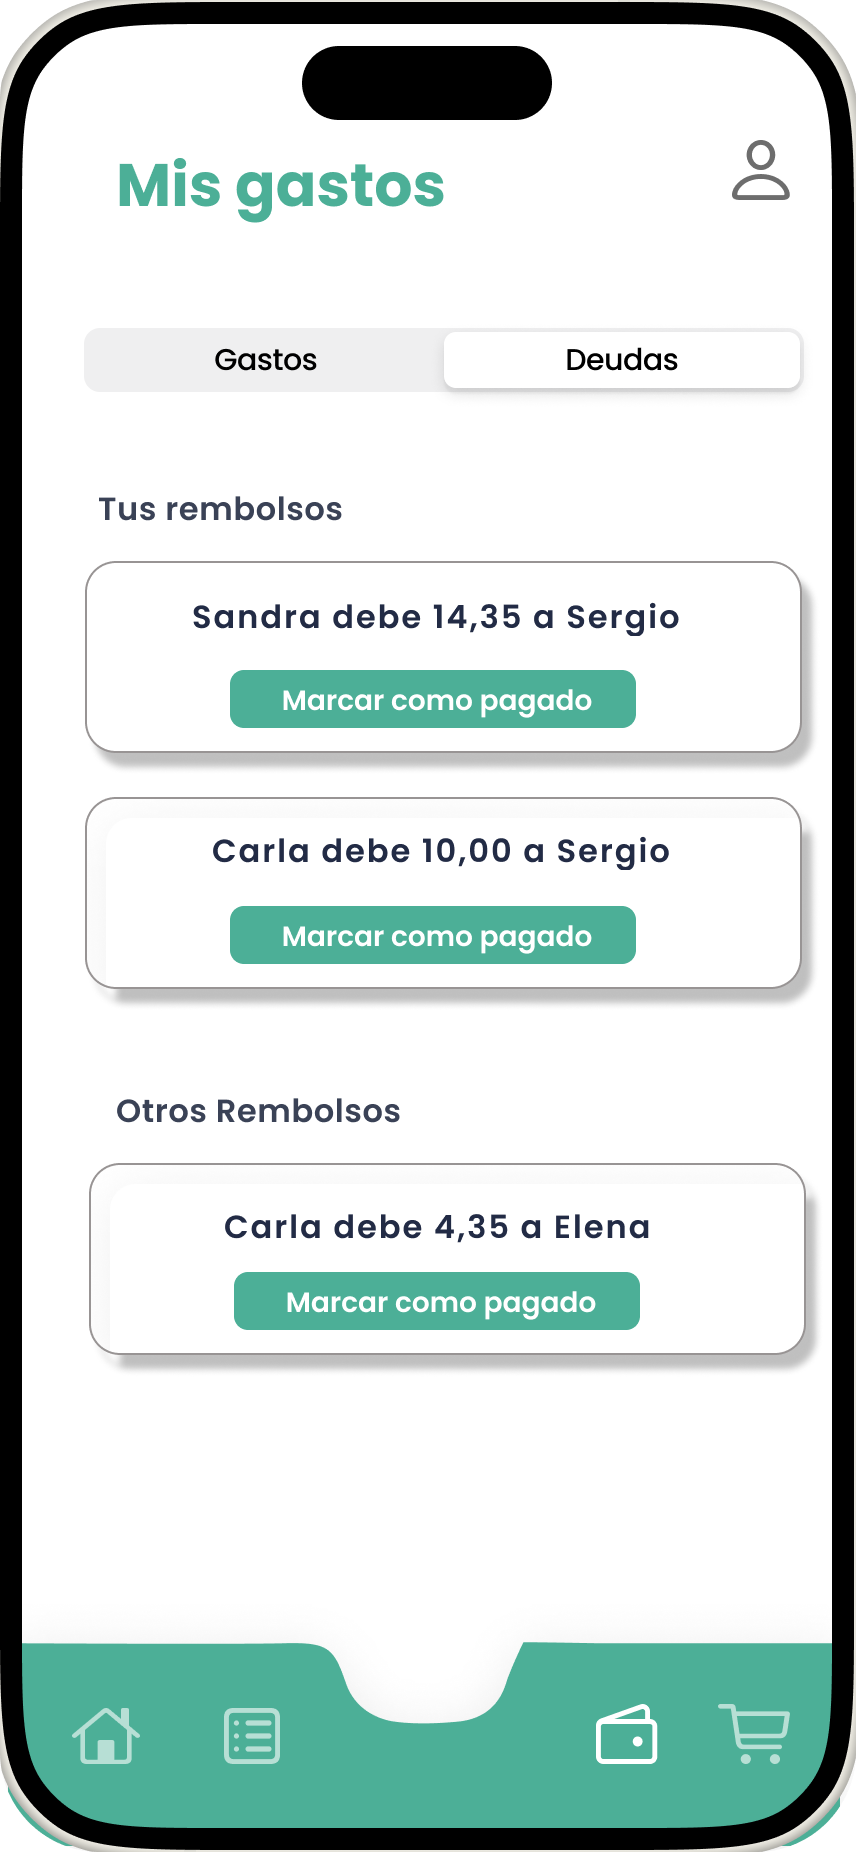
\includegraphics[width=0.45\textwidth]{../capitulos/img/pay_screen.png}
    \caption{Diseño de la pantalla para saldar deudas.}
    \label{settle_debts}
\end{figure}

\clearpage

\subsection{Interfaces de gráficas del Grupo 5: \textit{Gestión de la compra}}

\begin{figure}[ht]
    \centering
    \begin{minipage}{0.45\textwidth}
        \centering
        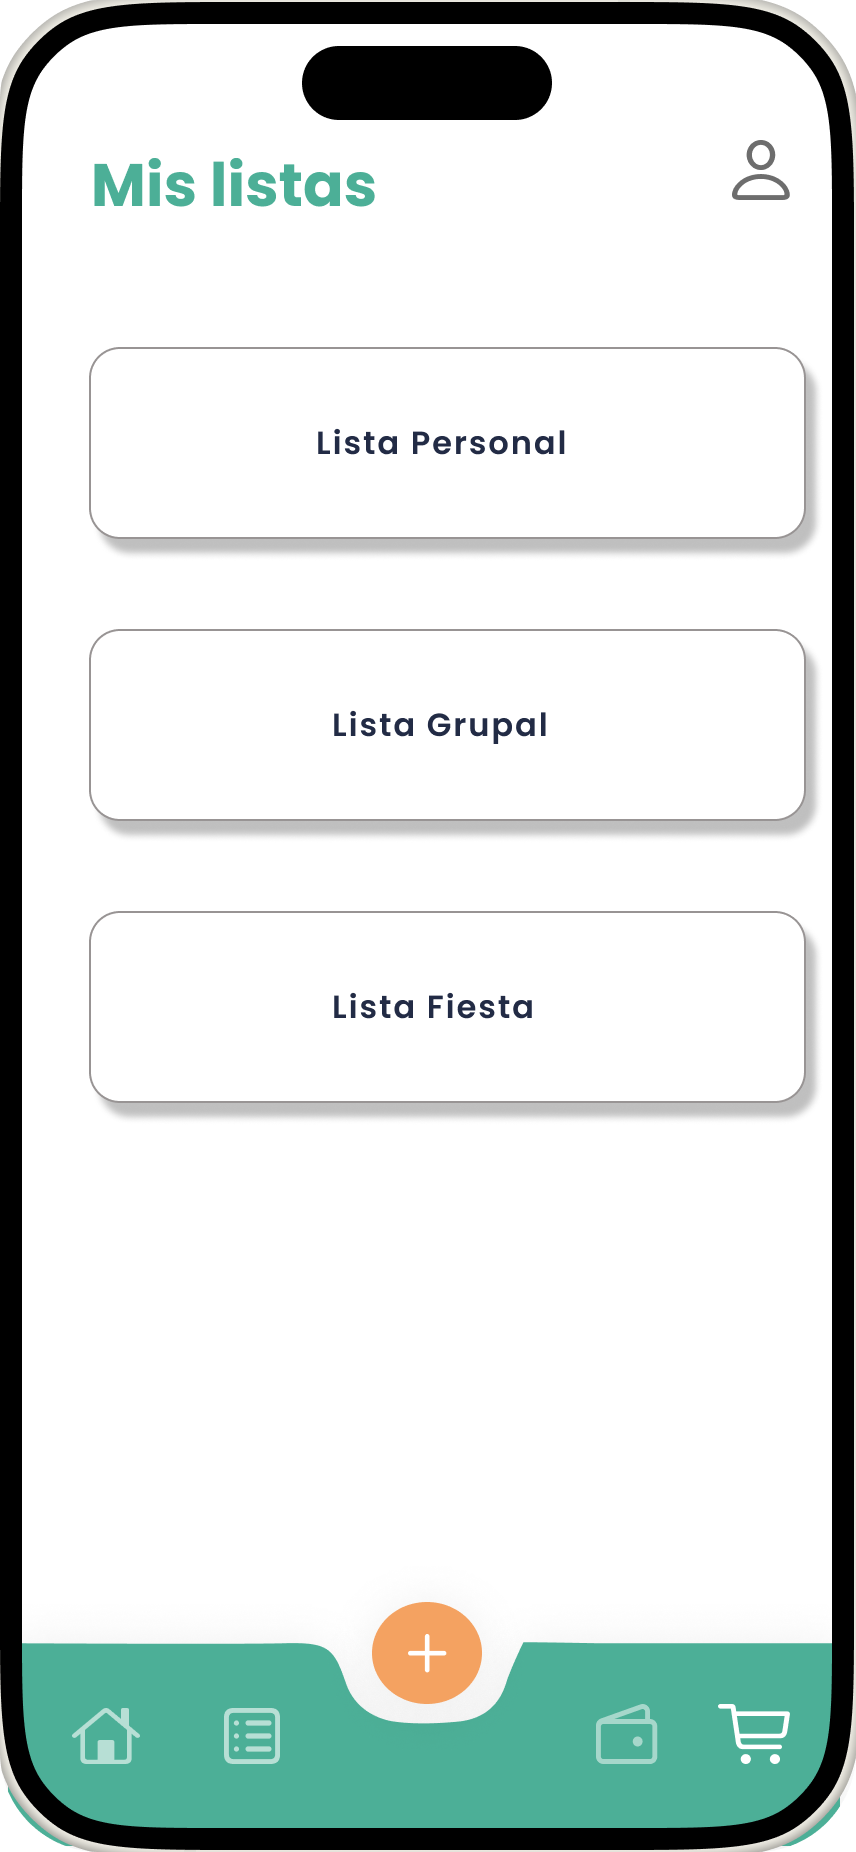
\includegraphics[width=\textwidth]{../capitulos/img/list_screen.png}
        \caption{Diseño de la pantalla de la lista de la compra.}
        \label{shopping_list}
    \end{minipage}
    \hfill
    \begin{minipage}{0.45\textwidth}
        \centering
        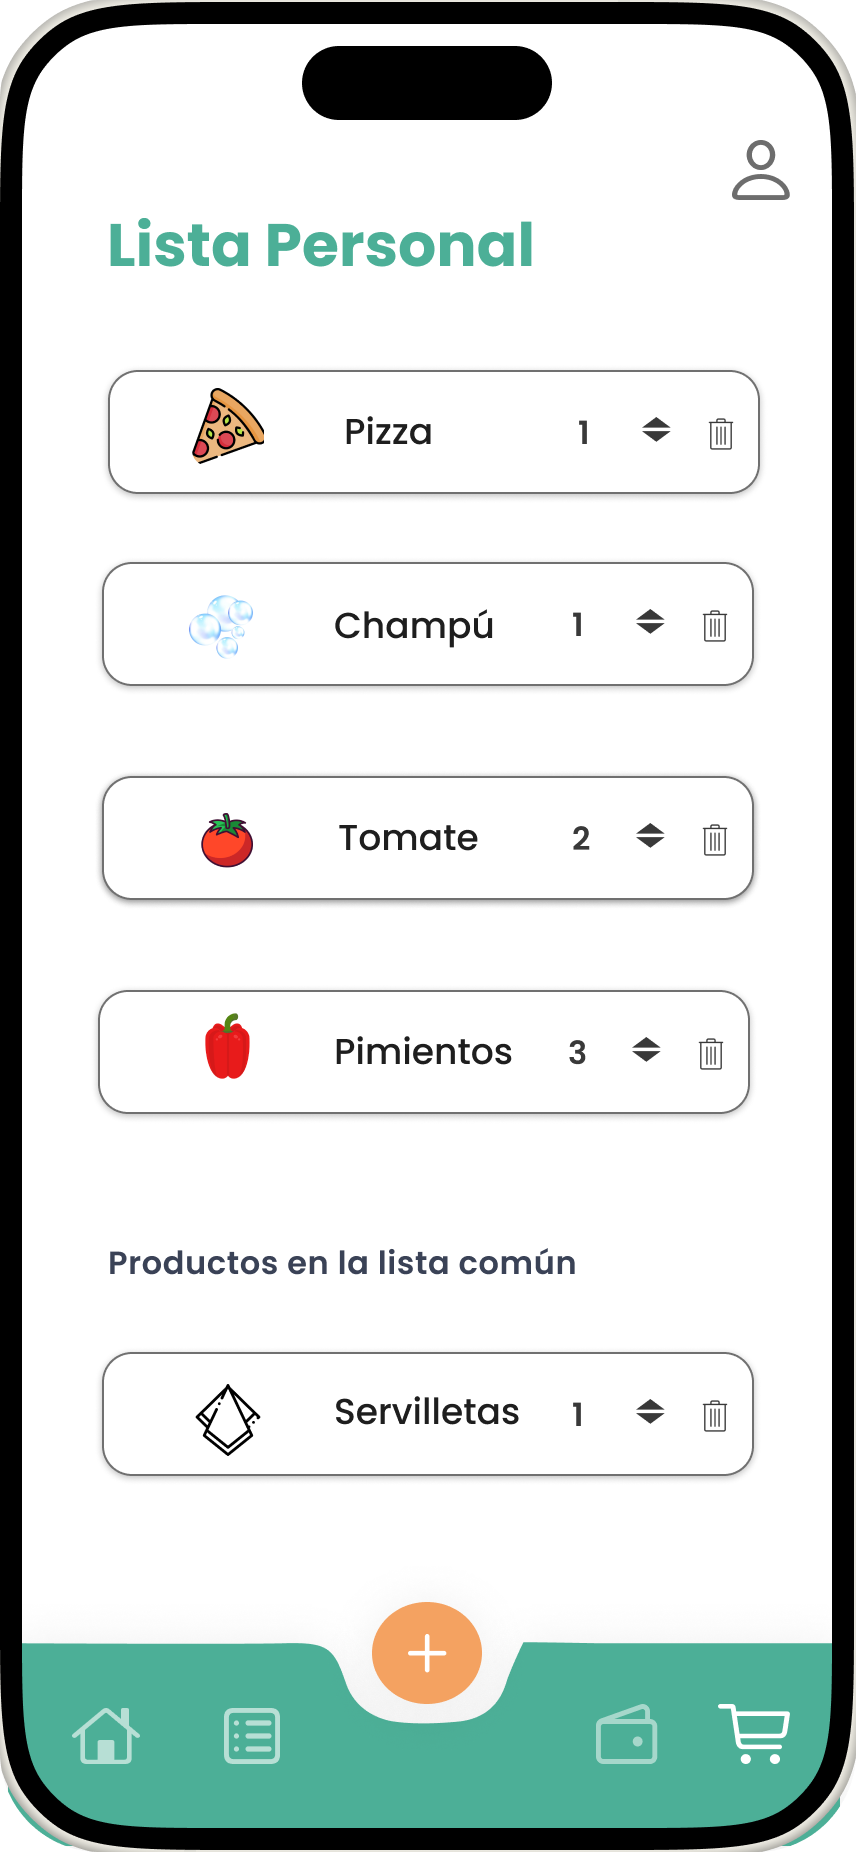
\includegraphics[width=\textwidth]{../capitulos/img/product_screen.png}
        \caption{Diseño de la pantalla de productos.}
        \label{products}
    \end{minipage}
\end{figure}

\newpage



\newpage

\bibliography{bibliografia.bib}
%\input{capitulos/05_Diseno}
%
%\input{capitulos/06_Implementacion}
%
%\input{capitulos/07_Pruebas}
%
%\input{capitulos/08_Conclusiones}
%
%%\chapter{Conclusiones y Trabajos Futuros}
%
%
%%\nocite{*}
%\bibliography{bibliografia/bibliografia}\addcontentsline{toc}{chapter}{Bibliografía}
%\bibliographystyle{miunsrturl}
%
%\appendix
%\input{apendices/manual_usuario/manual_usuario}
%%\input{apendices/paper/paper}
%\input{glosario/entradas_glosario}
% \addcontentsline{toc}{chapter}{Glosario}
% \printglossary
\chapter*{}
\thispagestyle{empty}

\end{document}
